\chapter{Results}
\label{chap:final-results}
This chapter reports the empirical findings obtained under the protocol described in Chapter~\ref{chap:final-methods}. It first documents the final cohort and experimental integrity, then presents training convergence, internal test-set outcomes, and the paired comparison between architectures. The chapter concludes with the external technical characterization and the blinded physician evaluation. Interpretation of these findings is reserved for Chapter~\ref{chap:final-discussion}.

\section{Final Group and Experimental Integrity}
\subsection{Final Group and Exclusion of Unmatched Pairs}

It is important to clarify the final results of the tracing and matching process. First of all, not all slices could be traced for the matching algorithm, but most of the data was successfully associated with the original exams. At the end of the direct and indirect matching steps, and before the complementary analysis with\acrshort{ms-ssim}, 11,942 of the 14,000 pairs provided by the\acrshort{ctmar} Dataset were traced to DeepLesion (including the 95 recovered by indirect matching), and 1,623 were traced to UCLH Stroke EIT. This totaled 13,565 pairs with associated metadata \Ref{tab:final-rastreio-msssim}.

\begin{table}[H]
    \centering
    \begin{tabular}{lccc}
        \hline
        \textbf{Dataset} & \textbf{Traced} & \textbf{Matched} & \textbf{Unmatched} \\
        \hline
        DeepLesion & 12,374 & 11,942 & 432 \\
        UCLH Stroke & 1,626  & 1,623  & 3   \\
        \hline
        \textbf{Total}  & \textbf{14,000} & \textbf{13,565} & \textbf{435} \\
        \hline
    \end{tabular}
    \centering
    \captionsetup{skip=2pt}
    \caption[Initial pair-matching screening]{Screening results before the complementary\acrshort{ms-ssim} analysis.}
    \label{tab:final-rastreio-msssim}
\end{table}
\subsection{Reported and Recovered Patient Counts}
\label{sec:reported-recovered-patient-counts}

The challenge paper reports that 12,227 body images were derived from approximately 1,230 DeepLesion patients and that 1,773 head images were derived from 10 UCLH Stroke EIT patients \cite{hanedaAAPMCTMetal2025}. The official downloaded package used in this study instead labels its 14,000 cases as 12,374 \texttt{body} and 1,626 \texttt{head}. The difference is exactly 147 cases in each stratum while preserving the total of 14,000. It is therefore compatible with some head-anatomy images having been packaged under \texttt{body}. This possibility is recorded as a dataset-level labelling discrepancy and is not treated as a reclassification made by this study.

The image-based traceability procedure recovered 258 distinct DeepLesion identifiers among the 11,939 retained \texttt{body} pairs and 11 Stroke EIT identifiers among the 1,623 retained \texttt{head} pairs, for 269 recovered source-patient identities. These are recovered identities, rather than an estimate of the complete source cohort. In particular, the discrepancy from the approximately 1,230 DeepLesion patients cited by the authors does not demonstrate that the remaining patients are absent: unmatched slices, conservative rejection of ambiguous candidates, source-image transformations, and the documented discrepancy between archive labels and the publication can all limit recovery. The published patient count was never used to accept a candidate or to change the patient-level partition.

In the evaluation step through\acrshort{ms-ssim}, among all pairs with a score below 0.90, only 3, previously associated with Deep Lesion, were rejected in the visual inspection \Ref{tab:final-tracking-post-msssim}.

\begin{table}[H]
    \centering
    \begin{tabular}{lccc}
        \hline
        \textbf{Dataset} & \textbf{Traced} & \textbf{Matched} & \textbf{Unmatched} \\
        \hline
        DeepLesion & 12,374 & 11,939 & 435 \\
        UCLH Stroke    & 1,626  & 1,623  & 3   \\
        \hline
        \textbf{Total}  & \textbf{14,000} & \textbf{13,562} & \textbf{438} \\
        \hline
    \end{tabular}
    \captionsetup{skip=2pt}
    \caption[Pair matching after MS-SSIM review]{Pair matching results after the complementary MS-SSIM analysis.}
    \label{tab:final-tracking-post-msssim}
\end{table}

Due to the fact that a significant amount of the data could be traced with high reliability, the remaining cases that could not be safely grouped were excluded from the training and validation process. In total, 438 pairs were removed for not having sufficient information to ensure safe grouping at the patient level. Among them were the 3 pairs rejected for being false positives in the evaluation step via\acrshort{ms-ssim}. All pairs removed from this study were visually inspected to confirm the absence of correspondence, ensuring that the exclusion was justified. 

Out of the pairs submitted in\acrshort{ms-ssim} review, 3 were added to the exclusion list. Then, out of the 14,000 pairs originally provided by the\acrshort{ctmar} Dataset, 13,562 were included in this work, while 438 were excluded to preserve the integrity of the experimental partitioning and minimize the risk of data leakage.

\subsection{Automatic Approval and Manual Review Outcomes}

The final curation outcome of every pair in the\acrshort{ctmar} dataset was recovered from the canonical manifest. Retained pairs were classified as manually reviewed. All remaining retained pairs were classified as automatically retained. Pairs not included in the final group were classified as excluded after verification, matching the 438 pairs already identified above.
\begin{figure}[H]
    \centering
    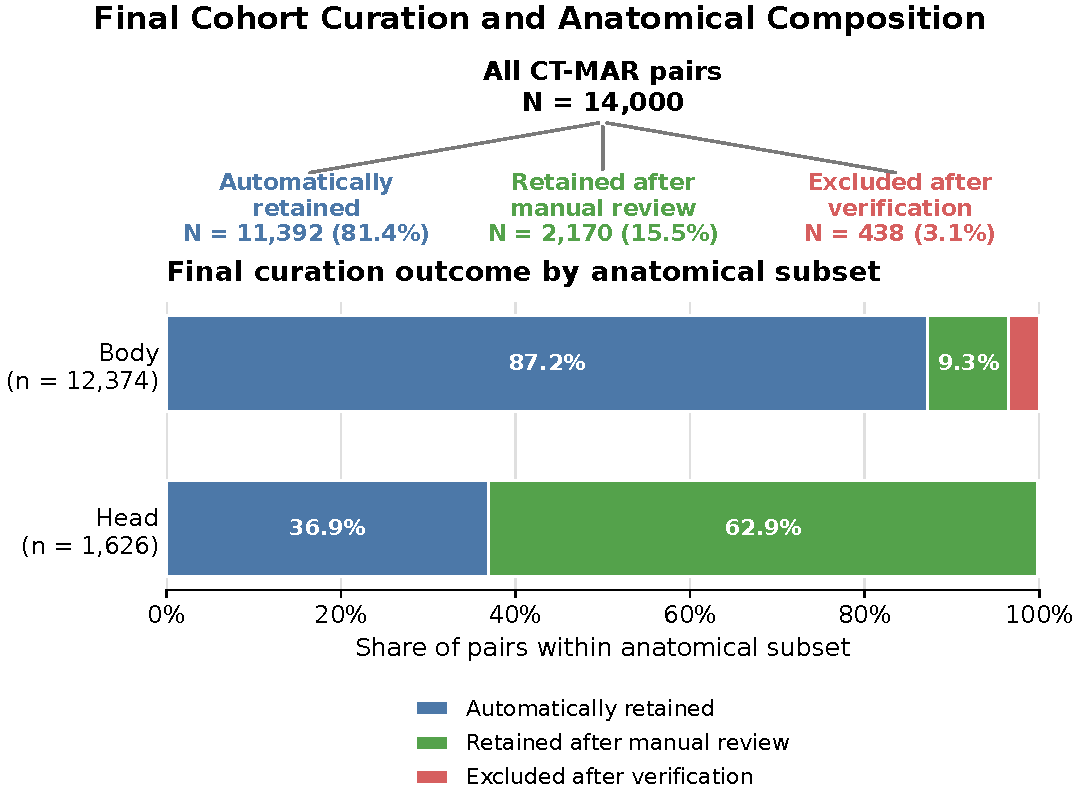
\includegraphics[width=0.80\textwidth]{Figures/Generated/final_cohort_curation_overview.pdf}
    \captionsetup{skip=2pt}
    \graphiccaption[Final group curation]{Final curation outcomes for all 14,000\acrshort{ctmar} pairs. The upper panel reports the global distribution of outcomes. The lower panel reports the percentage within each anatomical subset. The manifest labels distinguish \textit{Body} and \textit{Head} subsets, rather than the precise anatomical location of a metallic implant.}
    \label{fig:final-cohort-curation}
\end{figure}

\subsection{Complementary Analysis with\acrshort{ms-ssim}}

Before advancing to the analysis of the results of the artifact reduction models, another evaluation of the\acrshort{ctmar} x DeepLesion/Stroke EIT results was conducted to verify the quality of the automatic matches. This step is crucial to ensure an extra layer of confidence in the results obtained by the structural similarity comparison algorithm.
Every pair that had its match automatically approved due to its score being above 0.994 was reviewed by a new algorithm that calculates the\acrshort{ms-ssim} between the corresponding images. A histogram of the\acrshort{ms-ssim} distribution was generated, and pairs with scores below 0.9 were manually reviewed and either approved or rejected based on human evaluation.

\begin{figure}[H]
    \centering
    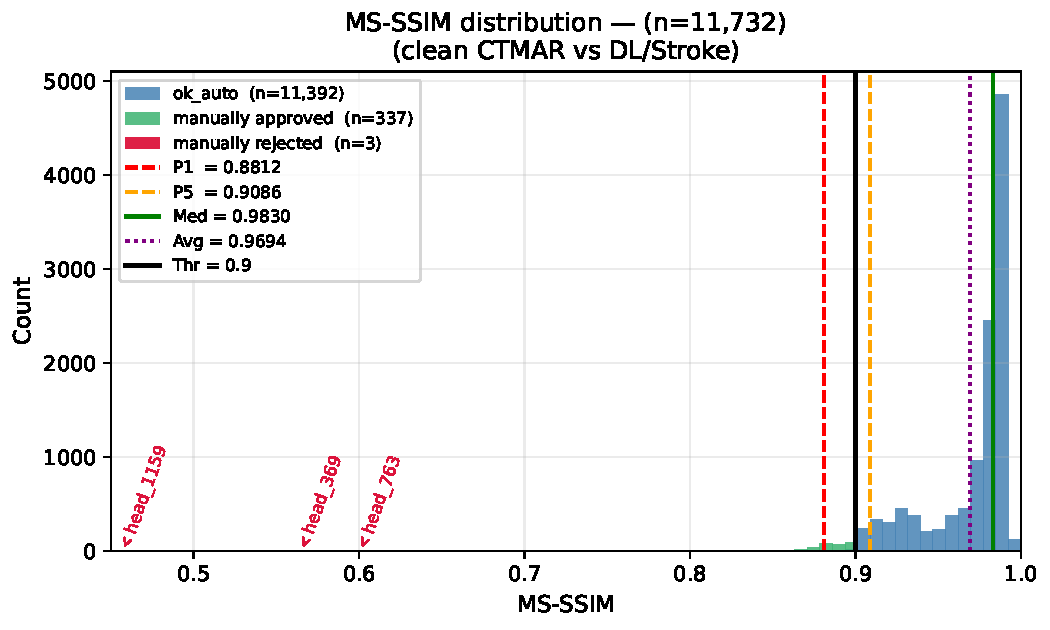
\includegraphics[width=\textwidth]{Figures/ssim_distribution_full.pdf} \\[4pt]
    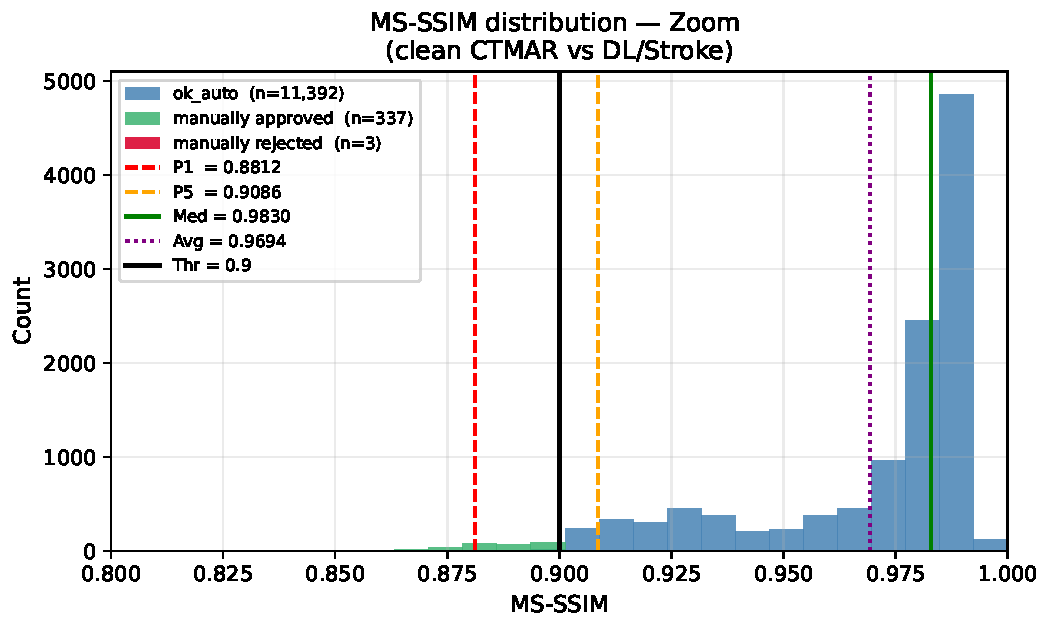
\includegraphics[width=\textwidth]{Figures/ssim_distribution_zoom.pdf}
    \captionsetup{skip=2pt}
    \graphiccaption[MS-SSIM distribution and zoom (clean CT-MAR vs DL/Stroke)]{\acrshort{ms-ssim} distribution between corresponding pairs (\acrshort{ctmar} vs DL/Stroke, automatically approved). Above: histogram with percentiles P1 and P5, median, mean, and threshold of 0.9. Below: zoom of the histogram for the region of greatest interest, highlighting pairs with\acrshort{ms-ssim} below 0.9, which were subject to manual review.}
    \label{fig:ssim_distribution}
\end{figure}

The distribution analysis between the corresponding pairs reveals that most pairs exhibit high structural similarity, with a mean value of 0.9694 and a median of 0.9830. This indicates that the automatic matching process is generally reliable and effective in identifying corresponding pairs between the\acrshort{ctmar} and DeepLesion/Stroke EIT datasets.

The pairs with\acrshort{ms-ssim} scores below 0.9 totaled 340, of which only 3 were rejected after human visual inspection \ref{fig:ECDF}. In this inspection, it was observed that even cases with quite low\acrshort{ms-ssim} scores were not false positives. Instead, they were due to differences in post-processing or general image treatment that generate local alterations to which\acrshort{ms-ssim} is more sensitive. This can be visualized in figure \ref{fig:manual_review_examples}. This fact highlights the effectiveness of the global structural similarity matching strategy adopted, which managed to identify pairs accurately, with only 3 false positives identified even after rigorous analysis \ref{fig:reproved_examples}. This shows that the methodology is robust and performed better in detecting slices in this work than using\acrshort{ms-ssim} itself. While local differences affected\acrshort{ms-ssim} more significantly, the cosine similarity-based methodology was able to identify correct matches with high global scores, even in cases of pronounced local differences.
\begin{figure}[H]
    \centering
    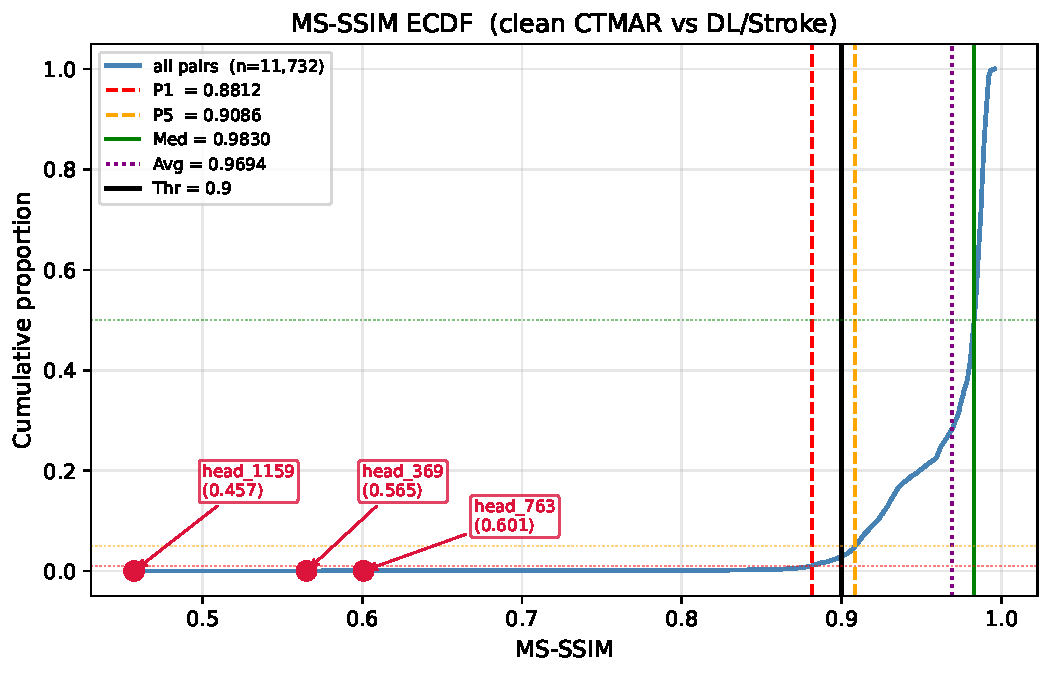
\includegraphics[width=\textwidth]{Figures/ssim_ecdf_final.pdf}
    \captionsetup{skip=2pt}
    \graphiccaption[MS-SSIM ECDF (clean CT-MAR vs DL/Stroke)]{\acrshort{ms-ssim} distribution between corresponding pairs (\acrshort{ctmar} vs DL/Stroke, automatically approved). Left: histogram with percentiles P1 and P5, median, mean, and threshold of 0.9. Right: corresponding ECDF. Pairs with MS-SSIM below 0.9 were subject to manual review.}
    \label{fig:ECDF}
\end{figure}

\begin{figure}[H]
    \centering
    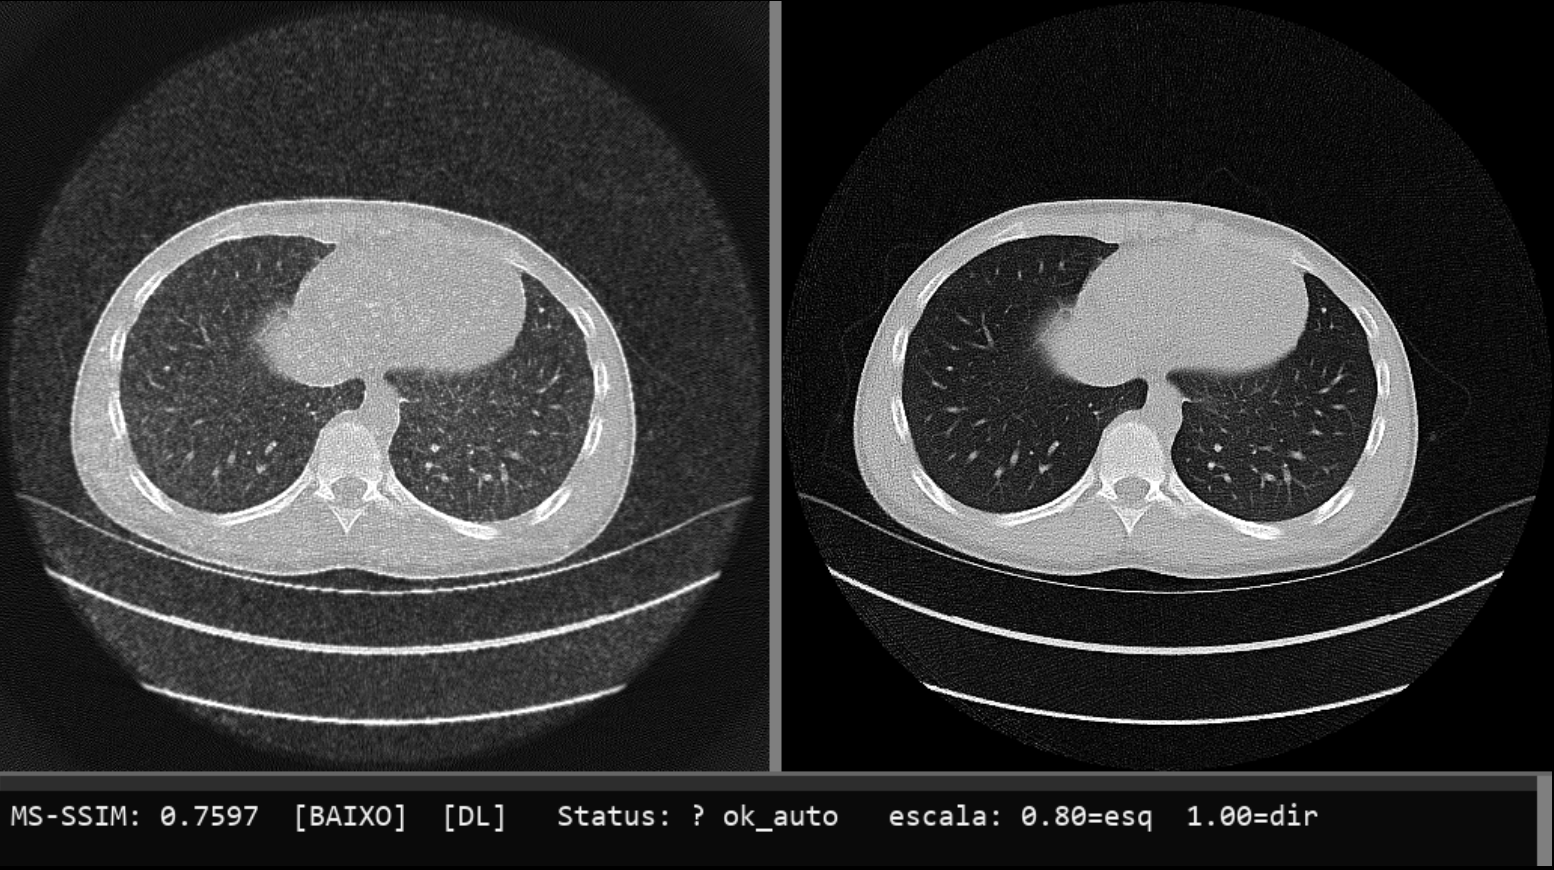
\includegraphics[width=0.70\textwidth]{Figures/image4.png}\\[2pt]
    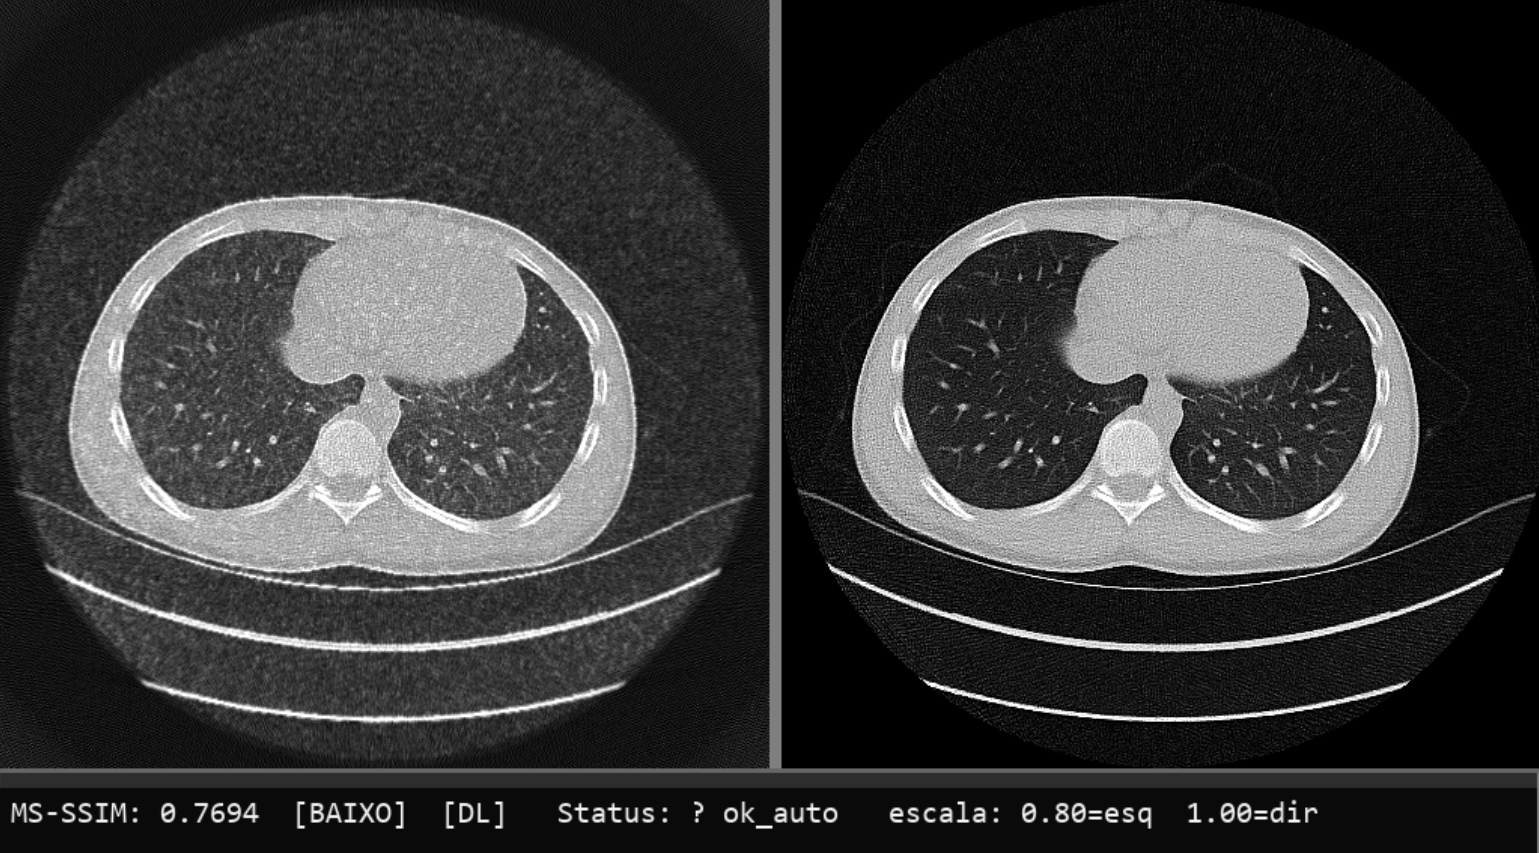
\includegraphics[width=0.70\textwidth]{Figures/image5.png}\\[2pt]
    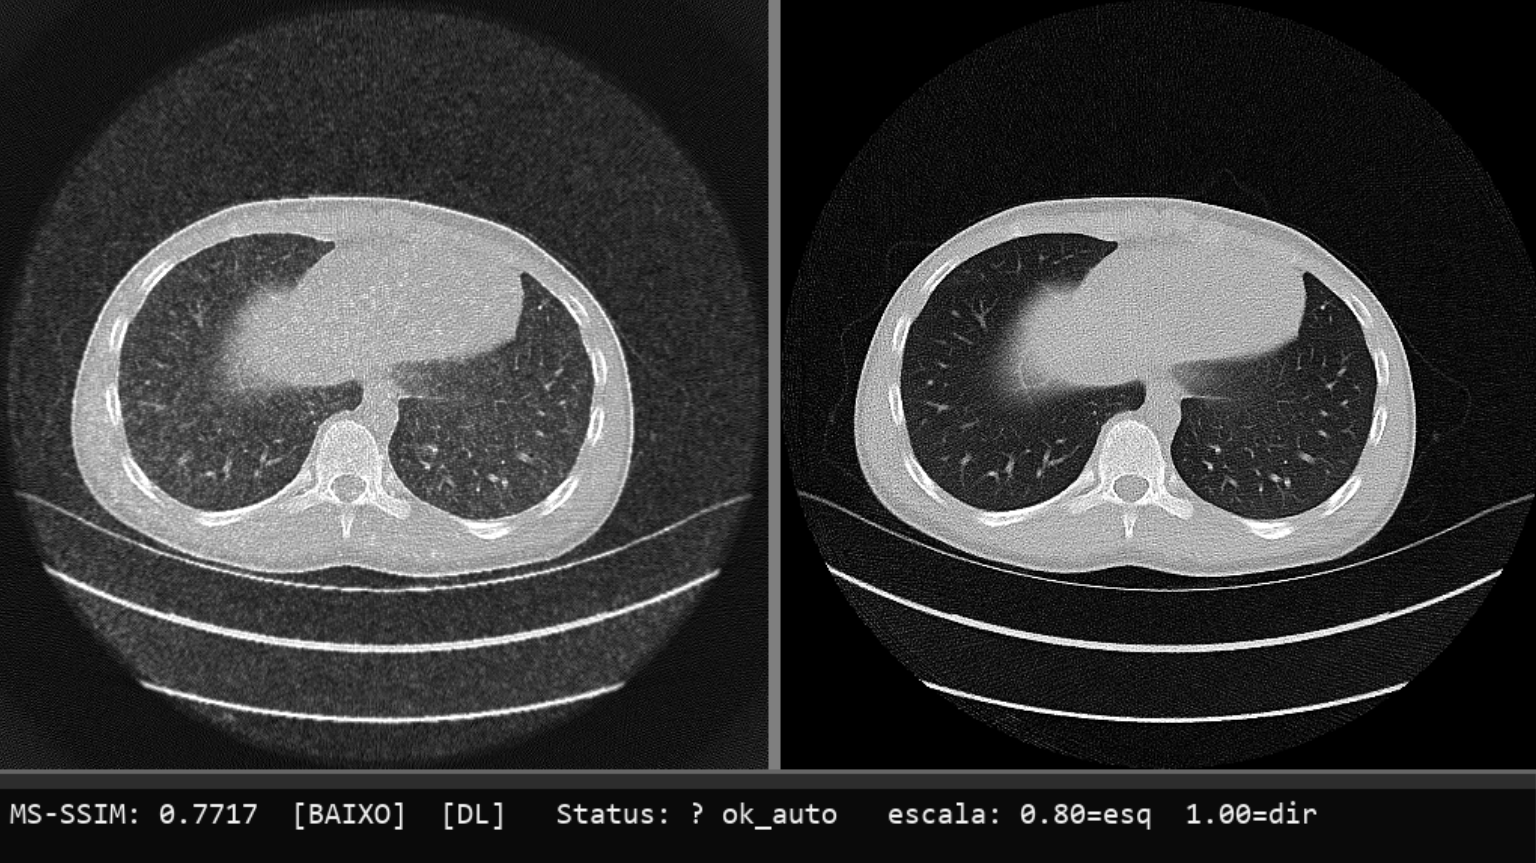
\includegraphics[width=0.70\textwidth]{Figures/image6.png}
    \captionsetup{skip=2pt}
    \caption[Visually approved low MS-SSIM pairs]{Examples of corresponding pairs with low\acrshort{ms-ssim} values (0.7597, 0.7694, and 0.7717, respectively) approved after human visual inspection despite low scores.}
    \label{fig:manual_review_examples}
\end{figure}

Clearly, the reproved pairs presented\acrshort{ms-ssim} values significantly below the standard (< 0.61), with extremely low scores, as shown in figure \ref{fig:reproved_examples}. Additionally, they represented pairs with scores closer to the automatic acceptance threshold of 0.994. This demonstrates that the cases where the method fails are clear outliers in\acrshort{ms-ssim} and remain precisely in the gray area prone to errors in the empirical determination of the automatic acceptance threshold. Furthermore, the reproved pairs have very particular visual characteristics, with backgrounds dominating the image and few visible anatomical structures, making structural similarity assessment more challenging due to the high homogeneity of visual features.
\begin{figure}[H]
    \centering
    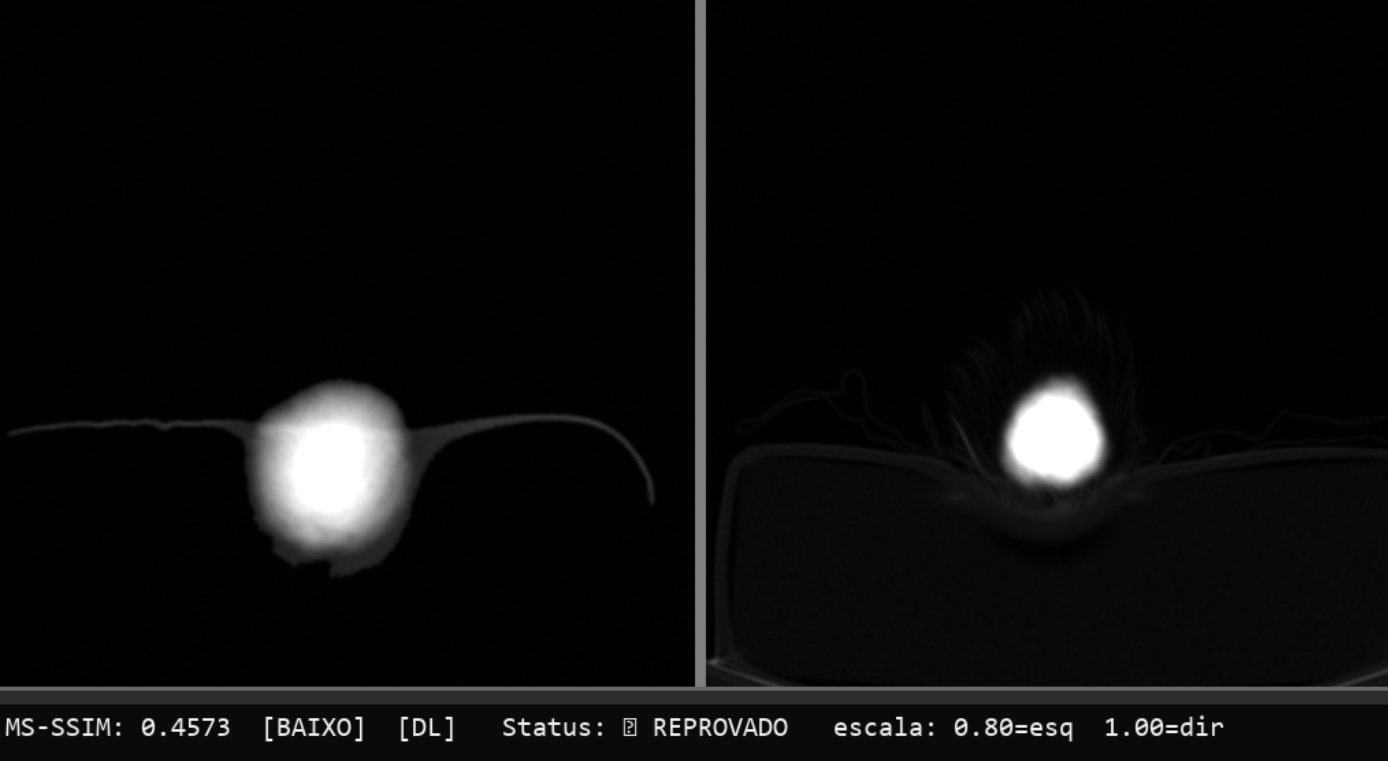
\includegraphics[width=0.70\textwidth]{Figures/image1.png}\\[4pt]
    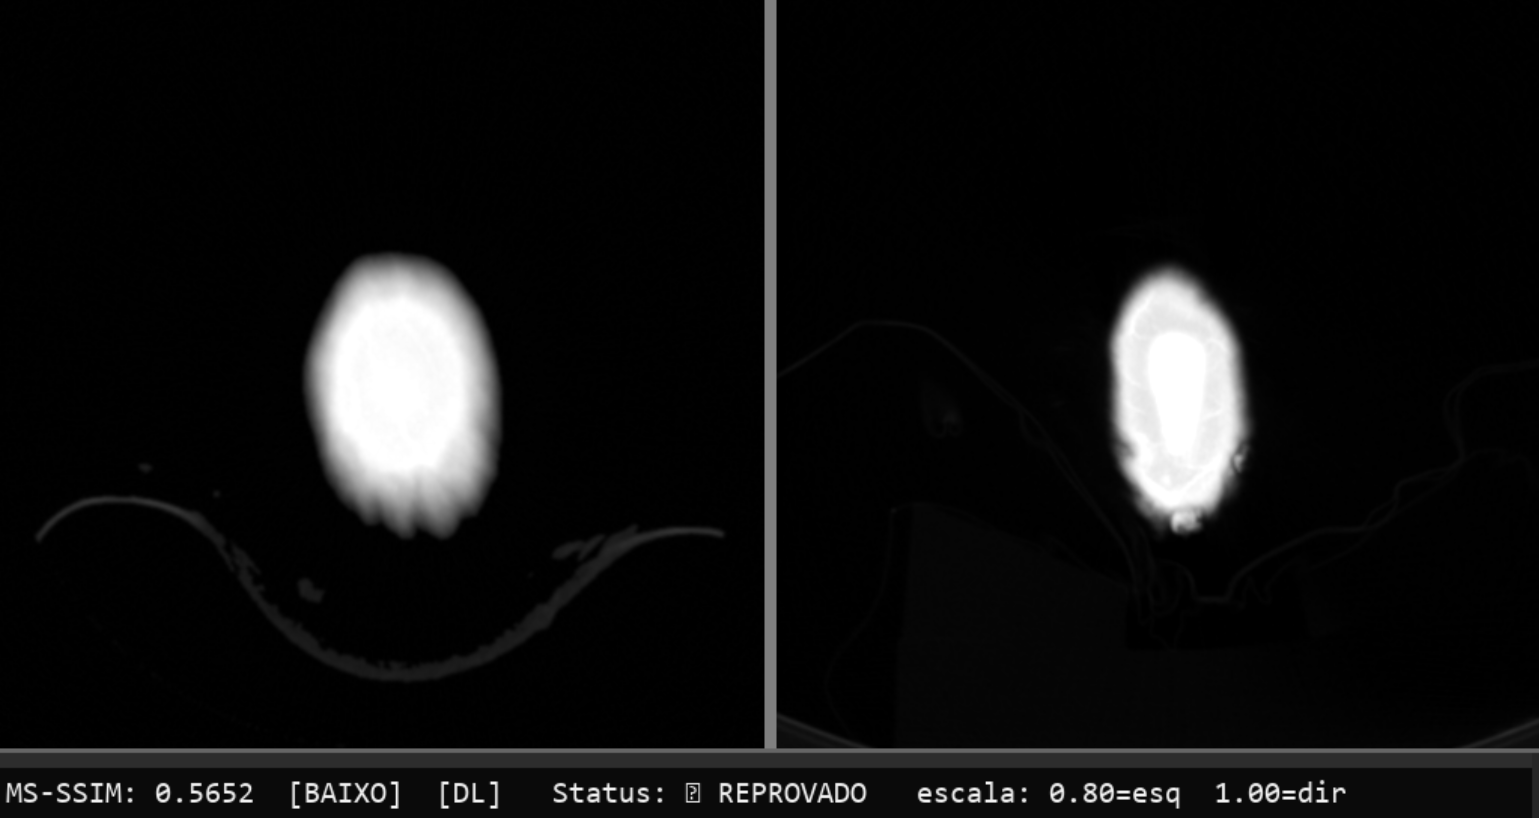
\includegraphics[width=0.70\textwidth]{Figures/image2.png}\\[4pt]
    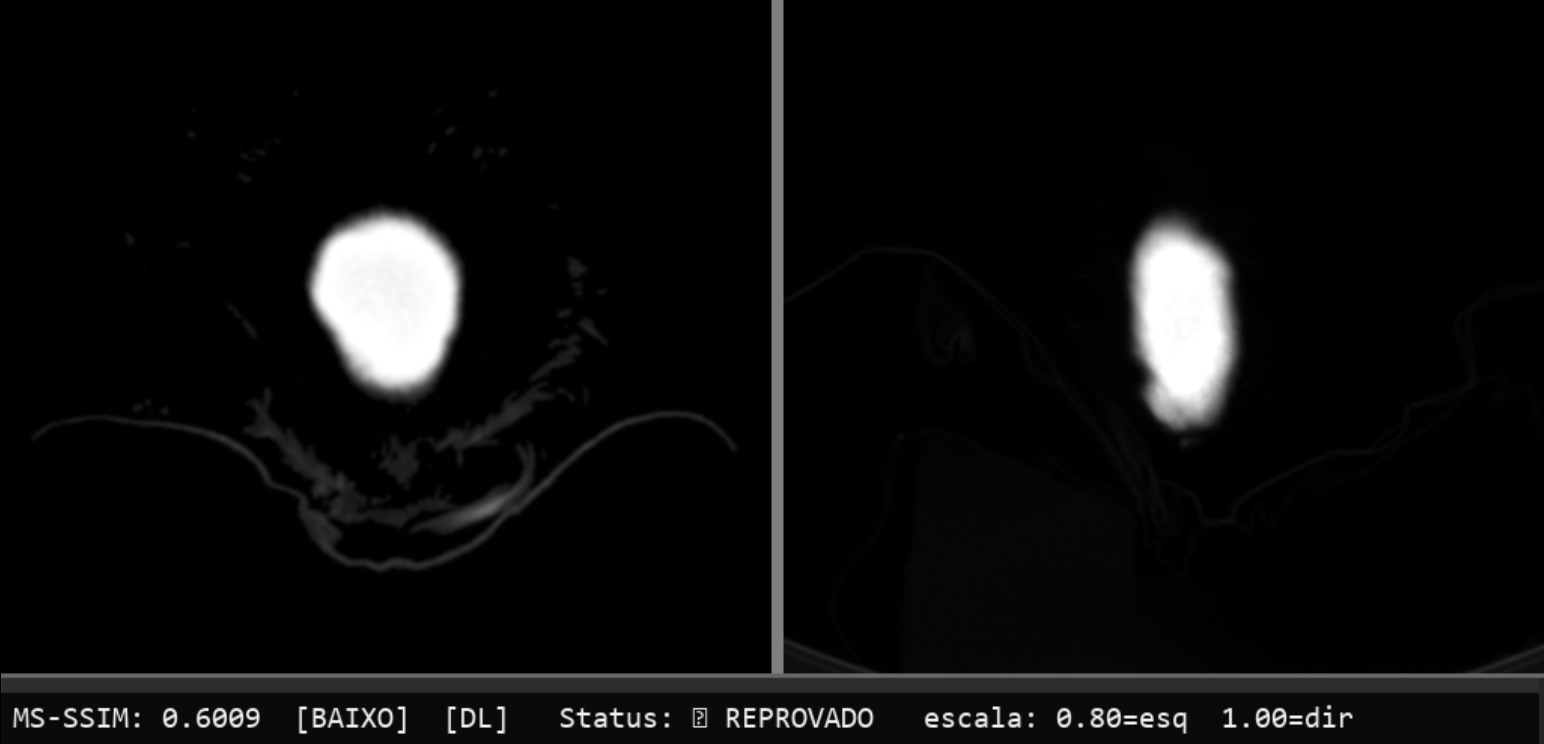
\includegraphics[width=0.70\textwidth]{Figures/image3.png}
    \captionsetup{skip=2pt}
    \caption[Visually rejected pairs]{Three reproved pairs after human visual inspection with\acrshort{ms-ssim} values (head\_1159: 0.4573, head\_369: 0.5652, and head\_763: 0.6009, respectively). The cosine similarity scores for these pairs were head\_1159: 0.9960, head\_369: 0.9952, and head\_763: 0.9951.}
    \label{fig:reproved_examples}
\end{figure}

\begin{figure}[H]
    \centering
    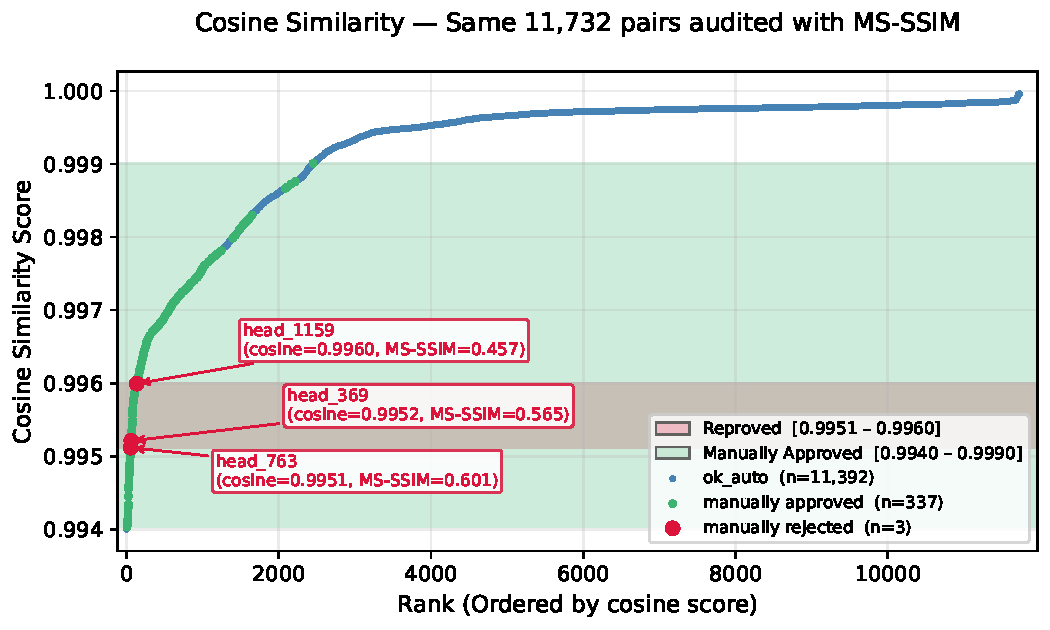
\includegraphics[width=0.98\textwidth]{Figures/cosine_scatter_audited.pdf}
    \captionsetup{skip=2pt}
    \graphiccaption[Cosine similarity of\acrshort{ms-ssim}-audited pairs]{Cosine similarity distribution of visually inspected pairs.}
    \label{fig:cosine_scatter_audited}
\end{figure}

The pairs with the most critical\acrshort{ms-ssim} scores just above the reproved ones had values greater than 0.75, demonstrating a clear distance between false positives and visually approved pairs. All inspected pairs with scores above this\acrshort{ms-ssim} value passed the visual inspection test. Since the pairs that did not undergo this scrutiny had scores above 0.90 in\acrshort{ms-ssim}, it is safe to assume that automatically approved pairs with scores above this threshold are reliable.

\begin{figure}[H]
    \centering
    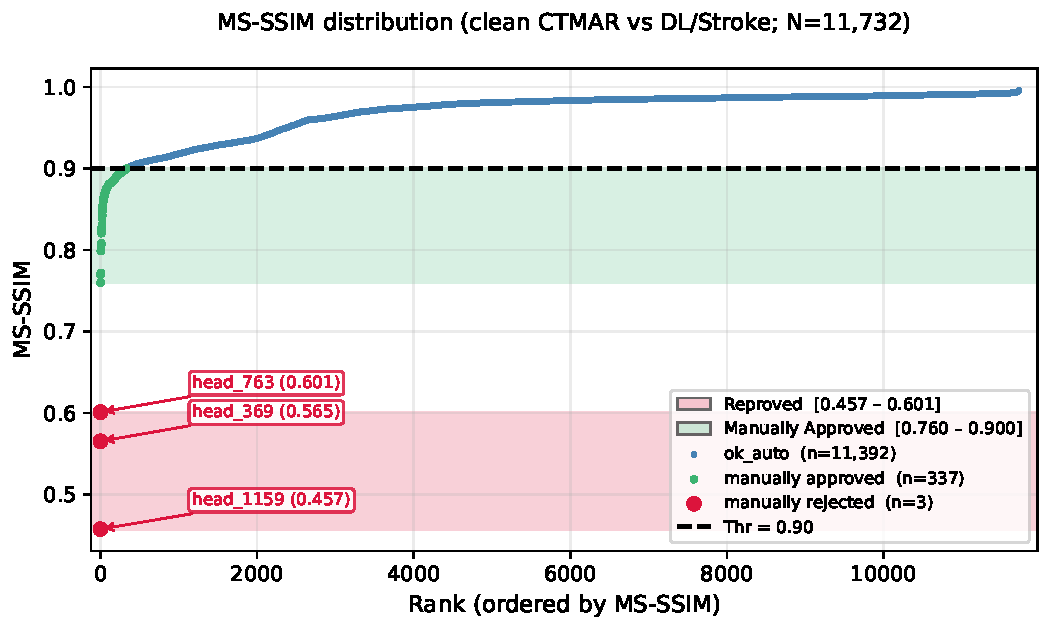
\includegraphics[width=0.95\textwidth]{Figures/ssim_scatter_dist.pdf}
    \captionsetup{skip=2pt}
    \graphiccaption[MS-SSIM distribution of audited pairs]{\acrshort{ms-ssim} values distribution for visually inspected pairs.}
    \label{fig:ssim_scatter_dist}
\end{figure}

In the direct search, 530 pairs did not obtain approved matches in either of the two source datasets. The complementary indirect matching step recovered 95 of these cases after visual inspection, leaving 435 pairs without secure matches. 

With relation to possible false negatives that could have resulted in unfair exclusion of pairs in this study, the adopted methodology was even more robust. Since there were few pairs that did not receive approval in either of the two source datasets, it was easy to visually verify each of these cases to confirm whether there was really no match or if the method failed to identify it. Of the 435 excluded pairs, 245 were excluded due to the automated criterion based on the threshold of 0.98. None of these cases were really false negatives, confirming once again the effectiveness of the adopted automatic matching method.
The other 190 pairs fell into the low-reliability score range (0.98 -- 0.994) and were marked as false matches at this stage. This highlights the importance of having determined a gray area of scores for which the automatic matching method is not efficient, and where human visual review becomes indispensable \ref{fig:score_distribution_bad}.
\begin{figure}[H]
    \centering
    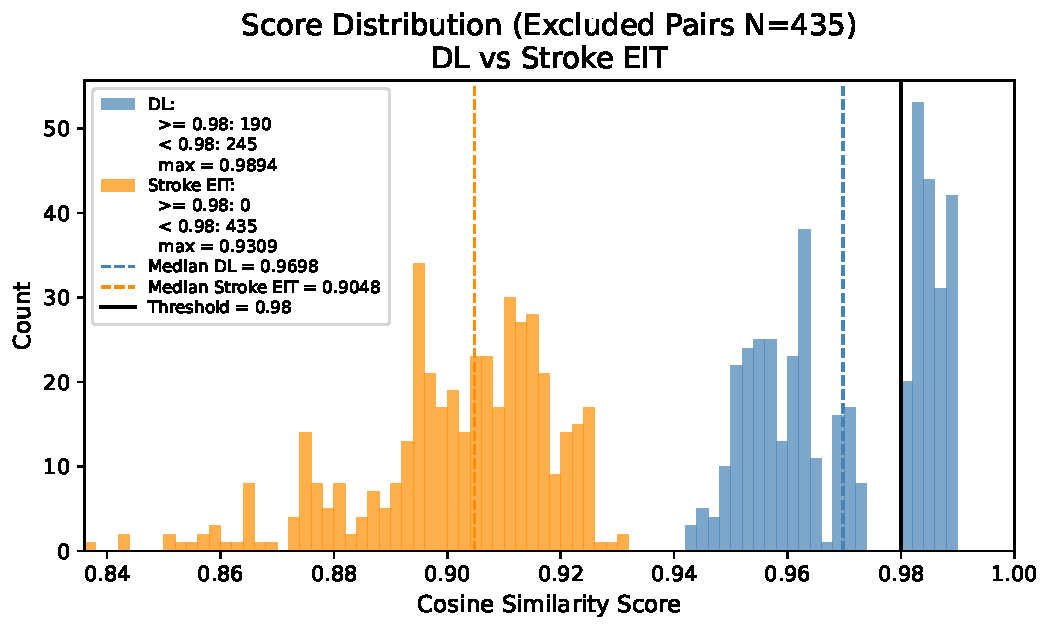
\includegraphics[width=0.98\textwidth]{Figures/score_distribution.pdf}
    \captionsetup{skip=2pt}
    \graphiccaption[Score distribution of excluded pairs: DL vs Stroke EIT]{Score distribution of excluded pairs (DL x Stroke EIT) for pairs without approved matches in either of the two source datasets (N=435). The orange histogram shows the distribution of scores for the 435 pairs rejected in the Stroke EIT Dataset. The blue histogram shows the distribution of the same 435 pairs rejected in the Deep Lesion Dataset.}
    \label{fig:score_distribution_bad}
\end{figure}


\subsection{Anatomical Distribution and Stratification}
\label{subsec:results-anatomical-distribution}

The anatomical proportion of 14,000 pairs in the\acrshort{ctmar} Dataset changed little after the screening and exclusion process of pairs with low reliability. Of the 438 removed cases, 435 were of the \textit{body} type and 3 of the \textit{head} type. The anatomical distribution of the pairs at the slice level included in the study is as follows:

\begin{itemize}
    \item \textbf{Body}: approximately 88.03\% ;
    \item \textbf{Head}: approximately 11.97\% .
\end{itemize}

The anatomical distribution of the pairs at the patient level included is found below:
\begin{itemize}
    \item \textbf{Body}: approximately 95.9\% (258/269 patients);
    \item \textbf{Head}: approximately 4.1\% (11/269 patients).
\end{itemize}

After partitioning, the train, validation, and test subsets had the following distribution:
\begin{table}[H]
    \centering
    \begin{tabular}{lcccc}
        \hline
        \textbf{Split} & \textbf{Body} & \textbf{Head}  &\textbf{\% Body} & \textbf{\% Head} \\
        \hline
        Train & 180 & 7 & 96.3\% & 3.7\% \\
        Val   & 39  & 2  & 95.1\% & 4.9\% \\
        Test  & 39  & 2  & 95.1\% & 4.9\% \\
        \hline
        \textbf{Total} & \textbf{258} & \textbf{11} & \textbf{--} & \textbf{--} \\
        \hline
    \end{tabular}
    \captionsetup{skip=2pt}
    \caption[Patient-level anatomical distribution by split]{Patient-level anatomical distribution by split.}
    \label{tab:final-split-anatomic}
\end{table}

\begin{table}[H]
    \centering
    \begin{tabular}{lccc}
        \hline
        \textbf{Split} & \textbf{Patients} & \textbf{\% Total}\\
        \hline
        Train  & 187 & 69.52\%\\
        Val    & 41 & 15.24\%\\
        Test   & 41 & 15.24\%\\
        \hline
        \textbf{Total} & \textbf{269} & \textbf{100\%} \\
        \hline
    \end{tabular}
    \captionsetup{skip=2pt}
    \caption[Patient distribution by split]{Patient distribution by split.}
    \label{tab:final-split-patient-subset}
\end{table}
\FloatBarrier

Due to the large variation in the number of slices per patient, the anatomical distribution at the pair level is quite different from the distribution at the patient level (\ref{tab:final-split-pairs} and \ref{tab:final-split-pairs-subset}). The same occurs for the total pairs distribution. Thus, the proportion of $\sim$ 70/15/15 was maintained at the patient level, but at the pair level it does not follow exactly the same proportion.

\begin{table}[H]
    \centering
    \begin{tabular}{lcccccc}
        \hline
        \textbf{Split}  & \textbf{Body} & \textbf{Head}  & \textbf{\% Body} & \textbf{\% Head}\\
        \hline
        Train  & 8\,491 & 953 & 89.91\% & 10.09\%\\
        Val    & 2\,255 & 385 & 85.42\% & 14.58\%\\
        Test   & 1\,193 & 285 & 80.72\% & 19.28\%\\
        \hline
        \textbf{Total} & \textbf{11\,939} & \textbf{1\,623} & \textbf{--} & \textbf{--} \\
        \hline
    \end{tabular}
    \centering
    \captionsetup{skip=2pt}
    \caption[Pair distribution by split and anatomical category]{Pair distribution by split and anatomical category.}
    \label{tab:final-split-pairs}
\end{table}

\begin{table}[H]
    \centering
    \begin{tabular}{lccc}
        \hline
        \textbf{Split} & \textbf{Pairs} & \textbf{\% Total}\\
        \hline
        Train  & 9\,444 & 69.64\%\\
        Val    & 2\,640 & 19.47\%\\
        Test   & 1\,478 & 10.89\%\\
        \hline
        \textbf{Total} & \textbf{13\,562} & \textbf{100\%} \\
        \hline
    \end{tabular}
    \captionsetup{skip=2pt}
    \caption[Pair distribution by split]{Pair distribution by split.}
    \label{tab:final-split-pairs-subset}
\end{table}

\section{Model Training}
\subsection{Training Convergence and Per-Run Checkpoint Selection}

All six deterministic runs converged and terminated between epochs 38 and 47, after the learning rate reached its lower bound. The best validation\acrshort{ssim} values occurred between epochs 23 and 44, before training termination, supporting restoration of the best checkpoint weights rather than use of the final epoch.

The highest validation reconstruction\acrshort{ssim} was 0.95113, obtained by the Single Model with seed 2024 at epoch 33. At that same checkpoint, validation\acrshort{psnr} was 35.30099~dB and validation\acrshort{mae} was 17.19180~HU. These values show which checkpoint was chosen for this individual run. On their own, they did not decide which run would go forward to external evaluation: that choice was made afterwards, by comparing all six checkpoints on the internal test partition using the Artifact-ROI rule agreed on in advance.

The convergence curves for the two seed-2024 architectures are shown below. The complete set of six runs and the validation tables for all model--seed combinations are provided in \autoref{sec:appendix-training-details}.

% Generated by scripts/publish_workflow_results_to_thesis.py. Do not edit.
\begingroup
\setlength{\intextsep}{4pt}
\begin{figure}[htbp]
\centering
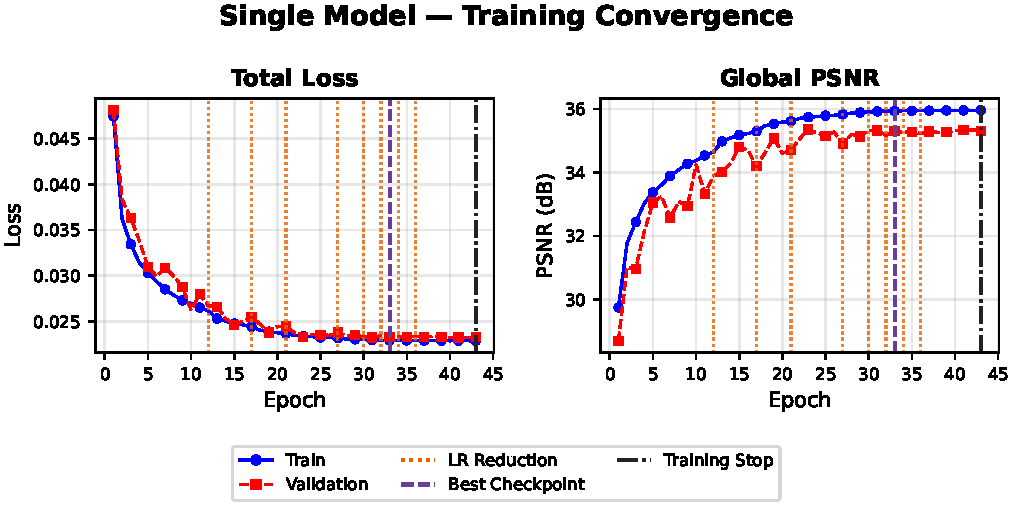
\includegraphics[width=0.98\linewidth]{Figures/Generated/training/training-curves-singlehead-pair-01-loss-psnr-6e359ebd.pdf}
\end{figure}

\begin{figure}[htbp]
\centering
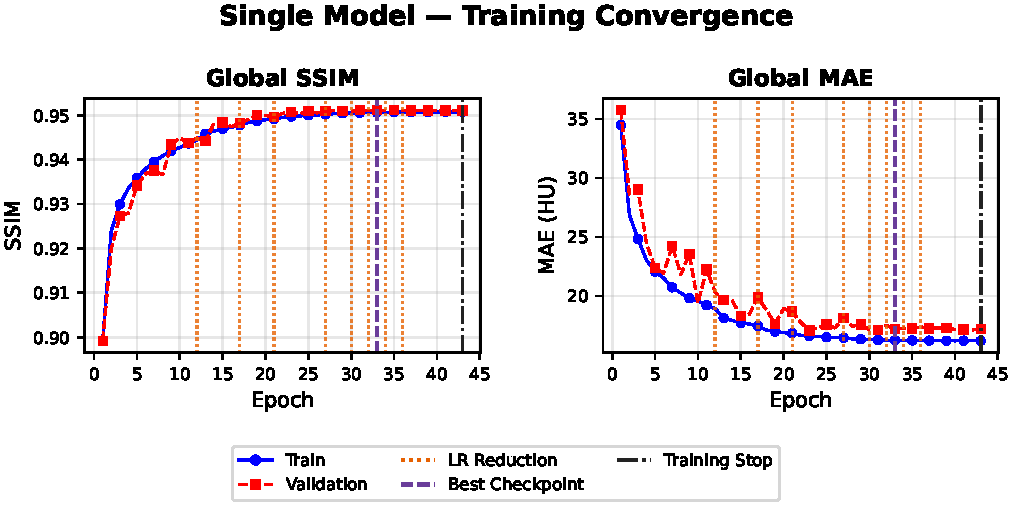
\includegraphics[width=0.98\linewidth]{Figures/Generated/training/training-curves-singlehead-pair-02-ssim-mae-80362d3f.pdf}
\end{figure}

\begin{figure}[htbp]
\centering
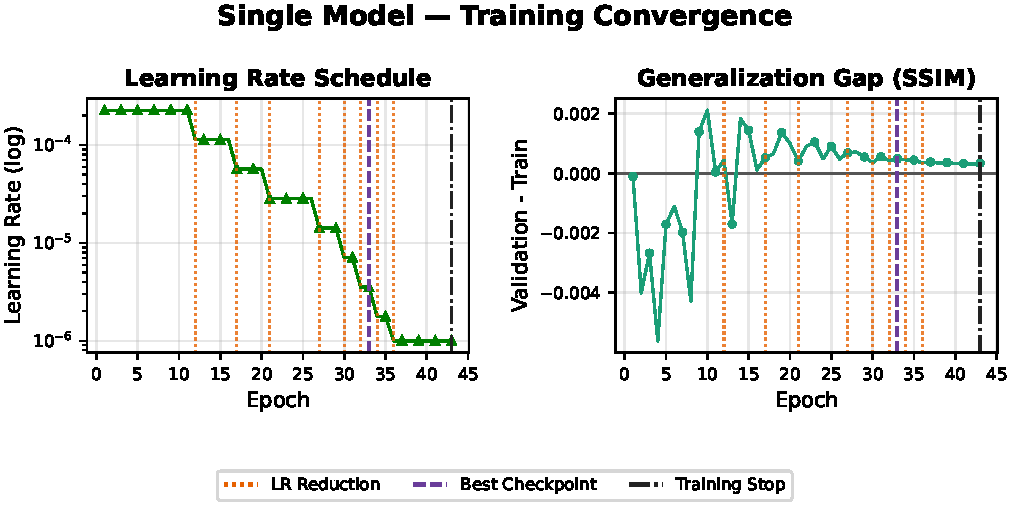
\includegraphics[width=0.98\linewidth]{Figures/Generated/training/training-curves-singlehead-pair-03-lr-gap-c975e425.pdf}
\end{figure}

\FloatBarrier
\captionsetup{skip=1.5pt}
\graphiccaptionof[Training convergence (results): Single Model, seed 2024]{Training convergence for the Single Model, seed 2024. Each chart pair repeats the shared legend so it remains interpretable if the group spans multiple pages. Orange dotted vertical lines indicate learning-rate reductions; the purple dashed line marks the epoch of the best validation checkpoint; and the black dash-dotted line marks training termination. The \textit{generalization-gap} panel reports validation minus training SSIM and supports inspection for persistent divergence compatible with overfitting.}
\label{fig:results-training-convergence-single-model-seed-2024}
\par\medskip
\endgroup

\begingroup
\setlength{\intextsep}{4pt}
\begin{figure}[htbp]
\centering
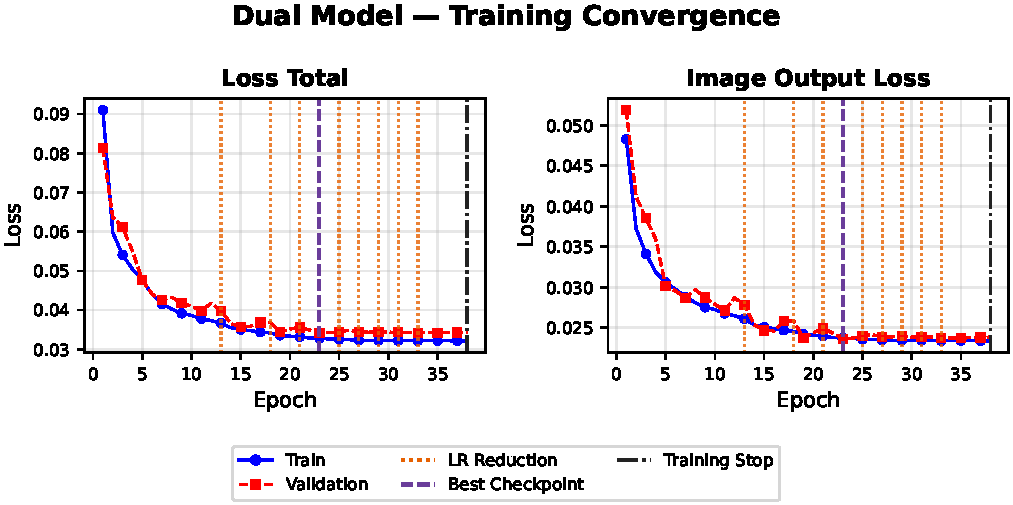
\includegraphics[width=0.98\linewidth]{Figures/Generated/training/training-curves-dualhead-pair-01-loss-419f6af3.pdf}
\end{figure}

\begin{figure}[htbp]
\centering
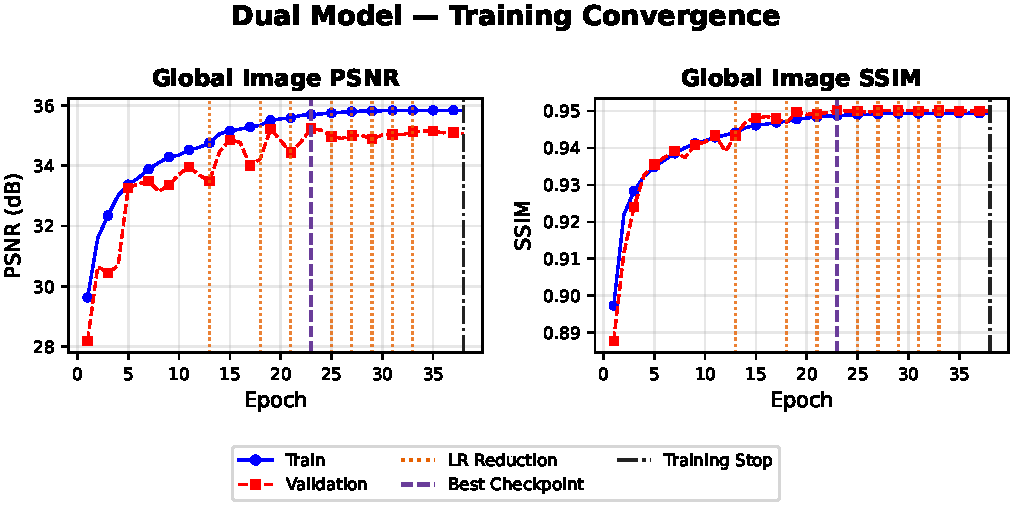
\includegraphics[width=0.98\linewidth]{Figures/Generated/training/training-curves-dualhead-pair-02-psnr-ssim-bc0a0156.pdf}
\end{figure}

\begin{figure}[htbp]
\centering
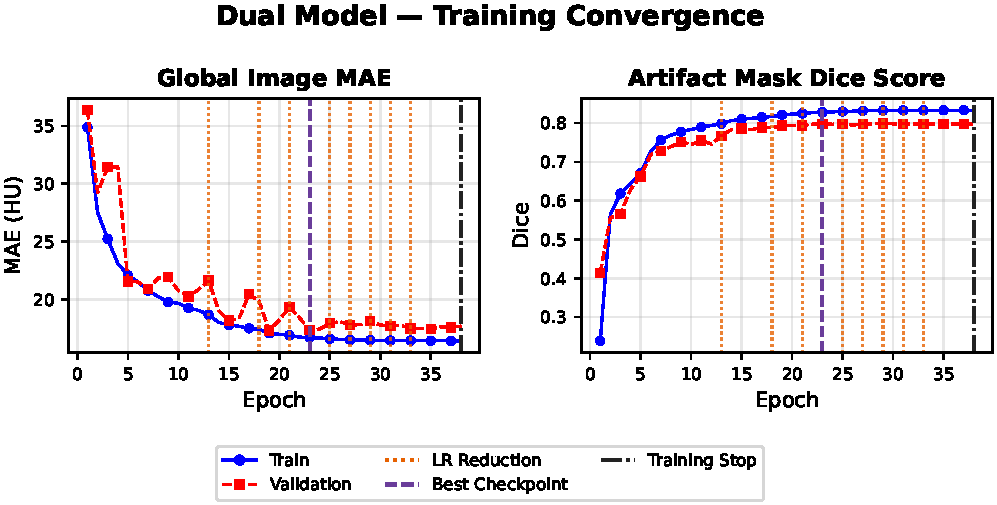
\includegraphics[width=0.98\linewidth]{Figures/Generated/training/training-curves-dualhead-pair-03-mae-dice-bde647ae.pdf}
\end{figure}

\begin{figure}[htbp]
\centering
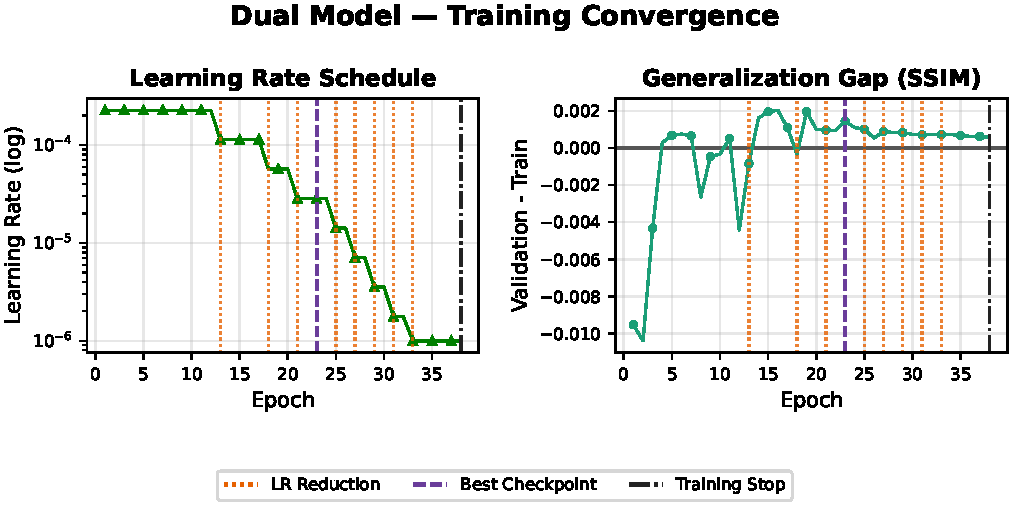
\includegraphics[width=0.98\linewidth]{Figures/Generated/training/training-curves-dualhead-pair-04-lr-gap-06e153c6.pdf}
\end{figure}

\FloatBarrier
\captionsetup{skip=1.5pt}
\graphiccaptionof[Training convergence (results): Dual Model, seed 2024]{Training convergence for the Dual Model, seed 2024. Each chart pair repeats the shared legend so it remains interpretable if the group spans multiple pages. Orange dotted vertical lines indicate learning-rate reductions; the purple dashed line marks the epoch of the best validation checkpoint; and the black dash-dotted line marks training termination. The \textit{generalization-gap} panel reports validation minus training SSIM and supports inspection for persistent divergence compatible with overfitting.}
\label{fig:results-training-convergence-dual-model-seed-2024}
\par\medskip
\endgroup




\section{Internal Evaluation in Test Subset}

The internal evaluation was conducted on the fixed test partition, composed of 1478 slices from 41 independent patients. For each checkpoint previously selected in validation,\acrshort{psnr},\acrshort{ssim}, and\acrshort{mae} were calculated between the reconstruction and the clean reference. All statistical comparisons used the patient, not the slice, as the unit of analysis: metrics were first averaged within each patient, and 95\% confidence intervals were obtained by resampling patients 10,000 times (a bootstrap procedure). The test set was not used to change any run's checkpoint. It was used once to compare the six validation-frozen candidates for the external-evaluation decision described in \autoref{sec:external-candidate-selection}.

\subsection{Region of Interest Evaluation}
\label{sec:roi-evaluation}

The regions of interest and the per-zone metric calculation followed the procedure described in \autoref{subsec:methods-roi}. This stratification makes it possible to separately quantify the correction in the region directly affected by artifacts and the changes introduced in body regions distant from the implant.

The final results, first aggregated per patient and then summarized over 41 independent patients, are presented in \autoref{tab:roi-delta-ssim}, \autoref{tab:roi-delta-psnr}, and \autoref{tab:roi-reducao-mae}. All six runs showed substantial improvement in the Artifact Zone: $\Delta$PSNR between 11.47 and 11.86~dB, $\Delta$SSIM between 0.322 and 0.328, and\acrshort{mae} reduction between 96.9 and 98.5~HU. In the Clean Zone, the mean changes were smaller ($\Delta$PSNR between 1.36 and 1.61~dB, $\Delta$SSIM between 0.057 and 0.058,\acrshort{mae} reduction between 3.2 and 3.6~HU). These changes should be interpreted as a quantitative description rather than as clinical validation of anatomical preservation.

\begin{table}[htbp]
    \centering
    \small
    \begin{tabular}{cccc}
        \multicolumn{4}{c}{\textbf{$\Delta$SSIM}} \\[4pt]
        \hline
        \textbf{Seed} & \textbf{Model} & \textbf{Artifact ROI} & \textbf{Clean ROI} \\
        \hline
        \multirow{2}{*}{42} & Single Model & $0.3276 \pm 0.0954$ & $0.0579 \pm 0.0426$ \\
                             & Dual Model   & $0.3233 \pm 0.0937$ & $0.0568 \pm 0.0421$ \\
        \hline
        \multirow{2}{*}{1337} & Single Model & $0.3278 \pm 0.0933$ & $0.0582 \pm 0.0421$ \\
                               & Dual Model   & $0.3224 \pm 0.0953$ & $0.0566 \pm 0.0422$ \\
        \hline
        \multirow{2}{*}{2024} & Single Model & $0.3279 \pm 0.0955$ & $0.0581 \pm 0.0422$ \\
                               & Dual Model   & $0.3266 \pm 0.0954$ & $0.0576 \pm 0.0422$ \\
        \hline
    \end{tabular}
    \captionsetup{skip=2pt}
    \caption[ROI $\Delta$SSIM]{$\Delta$SSIM by\acrshort{roi} on the test set. Values are mean $\pm$ standard deviation across patients ($n=41$).\tablecaptionnote{$\Delta\mathrm{SSIM}=\mathrm{SSIM}(\mathrm{Model},\mathrm{GT})-\mathrm{SSIM}(\mathrm{Input},\mathrm{GT})$ within the indicated ROI.}}
    \label{tab:roi-delta-ssim}
\end{table}
    
\begin{table}[htbp]
    \centering
    \small
    \begin{tabular}{cccc}
        \multicolumn{4}{c}{\textbf{$\Delta$PSNR (dB)}} \\[4pt]
        \hline
        \textbf{Seed} & \textbf{Model} & \textbf{Artifact ROI} & \textbf{Clean ROI} \\
        \hline
        \multirow{2}{*}{42} & Single Model & $11.75 \pm 2.59$ & $1.46 \pm 1.43$ \\
                             & Dual Model   & $11.65 \pm 2.53$ & $1.48 \pm 1.43$ \\
        \hline
        \multirow{2}{*}{1337} & Single Model & $11.84 \pm 2.54$ & $1.53 \pm 1.35$ \\
                               & Dual Model   & $11.47 \pm 2.57$ & $1.36 \pm 1.52$ \\
        \hline
        \multirow{2}{*}{2024} & Single Model & $11.86 \pm 2.69$ & $1.61 \pm 1.41$ \\
                               & Dual Model   & $11.84 \pm 2.62$ & $1.53 \pm 1.48$ \\
        \hline
    \end{tabular}
    \captionsetup{skip=2pt}
    \caption[ROI $\Delta$PSNR]{$\Delta$PSNR by\acrshort{roi} on the test set. Values are mean $\pm$ standard deviation across patients ($n=41$).\tablecaptionnote{$\Delta\mathrm{PSNR}=\mathrm{PSNR}(\mathrm{Model},\mathrm{GT})-\mathrm{PSNR}(\mathrm{Input},\mathrm{GT})$ within the indicated ROI.}}
    \label{tab:roi-delta-psnr}
\end{table}

\begin{table}[htbp]
    \centering
    \small
    \begin{tabular}{cccc}
        \multicolumn{4}{c}{\textbf{$\Delta$MAE (HU)}} \\[4pt]
        \hline
        \textbf{Seed} & \textbf{Model} & \textbf{Artifact ROI} & \textbf{Clean ROI} \\
        \hline
        \multirow{2}{*}{42} & Single Model & $97.8 \pm 19.6$ & $3.3 \pm 3.2$ \\
                             & Dual Model   & $97.5 \pm 19.1$ & $3.4 \pm 3.1$ \\
        \hline
        \multirow{2}{*}{1337} & Single Model & $98.5 \pm 19.6$ & $3.5 \pm 3.1$ \\
                               & Dual Model   & $96.9 \pm 19.9$ & $3.2 \pm 3.3$ \\
        \hline
        \multirow{2}{*}{2024} & Single Model & $98.4 \pm 20.2$ & $3.6 \pm 3.1$ \\
                               & Dual Model   & $98.3 \pm 19.8$ & $3.5 \pm 3.3$ \\
        \hline
    \end{tabular}
    \captionsetup{skip=2pt}
    \caption[ROI MAE reduction]{\acrshort{mae} reduction by\acrshort{roi} on the test set. Values are mean $\pm$ standard deviation across patients ($n=41$). Positive values correspond to error reduction.\tablecaptionnote{$\Delta\mathrm{MAE}=\mathrm{MAE}(\mathrm{Input},\mathrm{GT})-\mathrm{MAE}(\mathrm{Model},\mathrm{GT})$ within the indicated ROI. Positive values indicate error reduction.}}
    \label{tab:roi-reducao-mae}
\end{table}
\FloatBarrier

\subsection{Selection of the External-Evaluation Candidate}
\label{sec:external-candidate-selection}

Among the six validation-selected checkpoints, the Single Model with seed 2024 showed the greatest patient-level structural improvement in the Artifact Zone, while the corresponding change in the Clean Zone was substantially smaller. It was therefore selected for external evaluation. As no numerical equivalence margin was specified for the Clean Zone, this comparison does not constitute formal proof of anatomical safety. The remaining\acrshort{roi} and global metrics are complementary to this selection decision.

The \autoref{fig:roi-boxplots} and \autoref{fig:roi-safety} show the image-level distributions for the selected run. For clarity, the remaining plots present only this model. Data for all six runs are available in Appendix \ref{apendice:internal-evaluation}.

The box plots highlight the separation between the correction in the Artifact Zone and the smaller change in the Clean Zone. The scatter plot allows identification of heterogeneity between slices, including individual cases with unfavorable changes in the Clean Zone.

\FloatBarrier
\begingroup
\setlength{\intextsep}{4pt}
\begin{figure}[H]
    \centering
    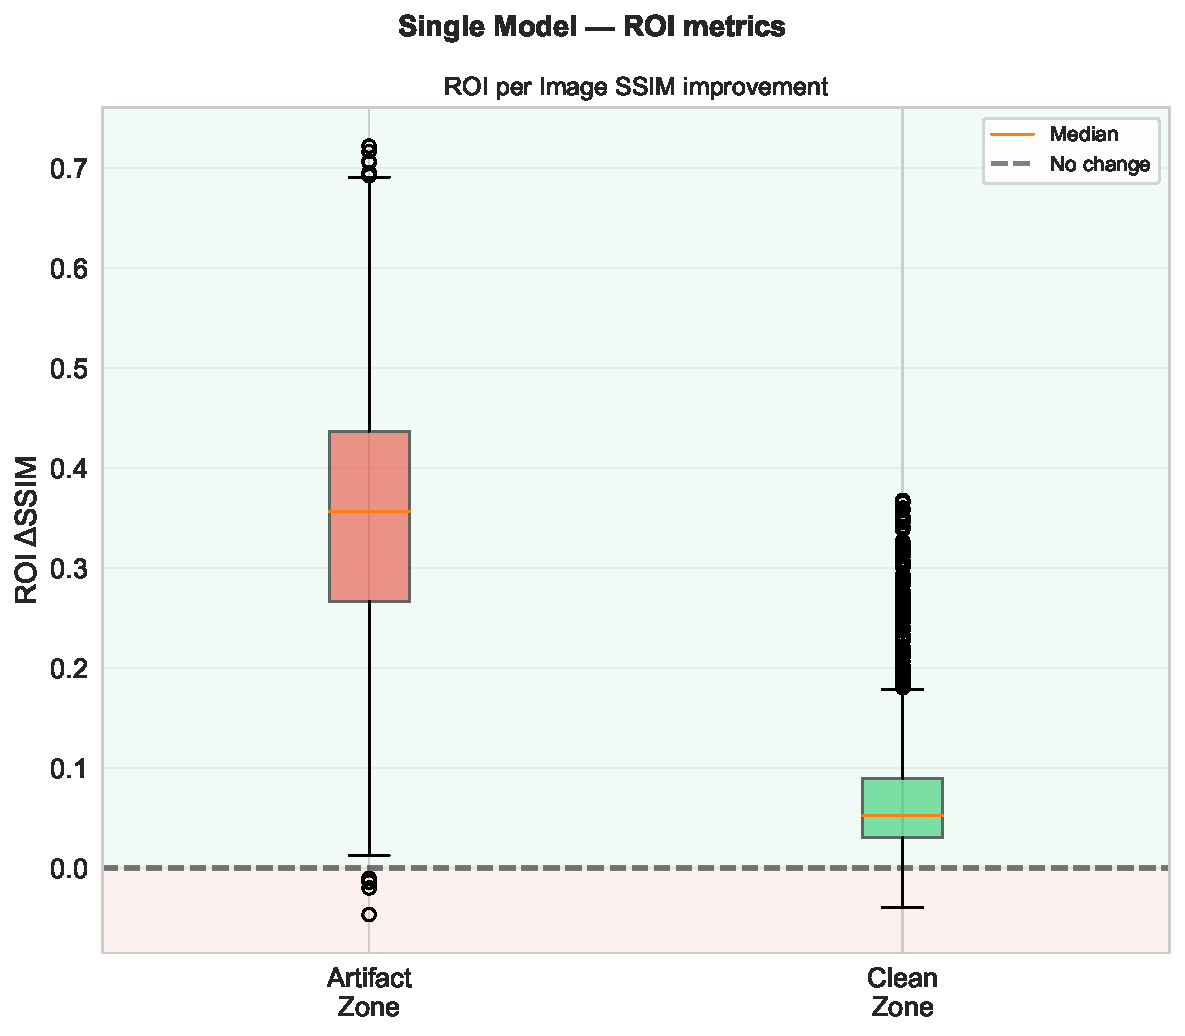
\includegraphics[width=0.84\linewidth]{Figures/Generated/evaluation_final/ROI/boxplot_roi_delta_ssim.pdf}
\end{figure}

\begin{figure}[H]
    \centering
    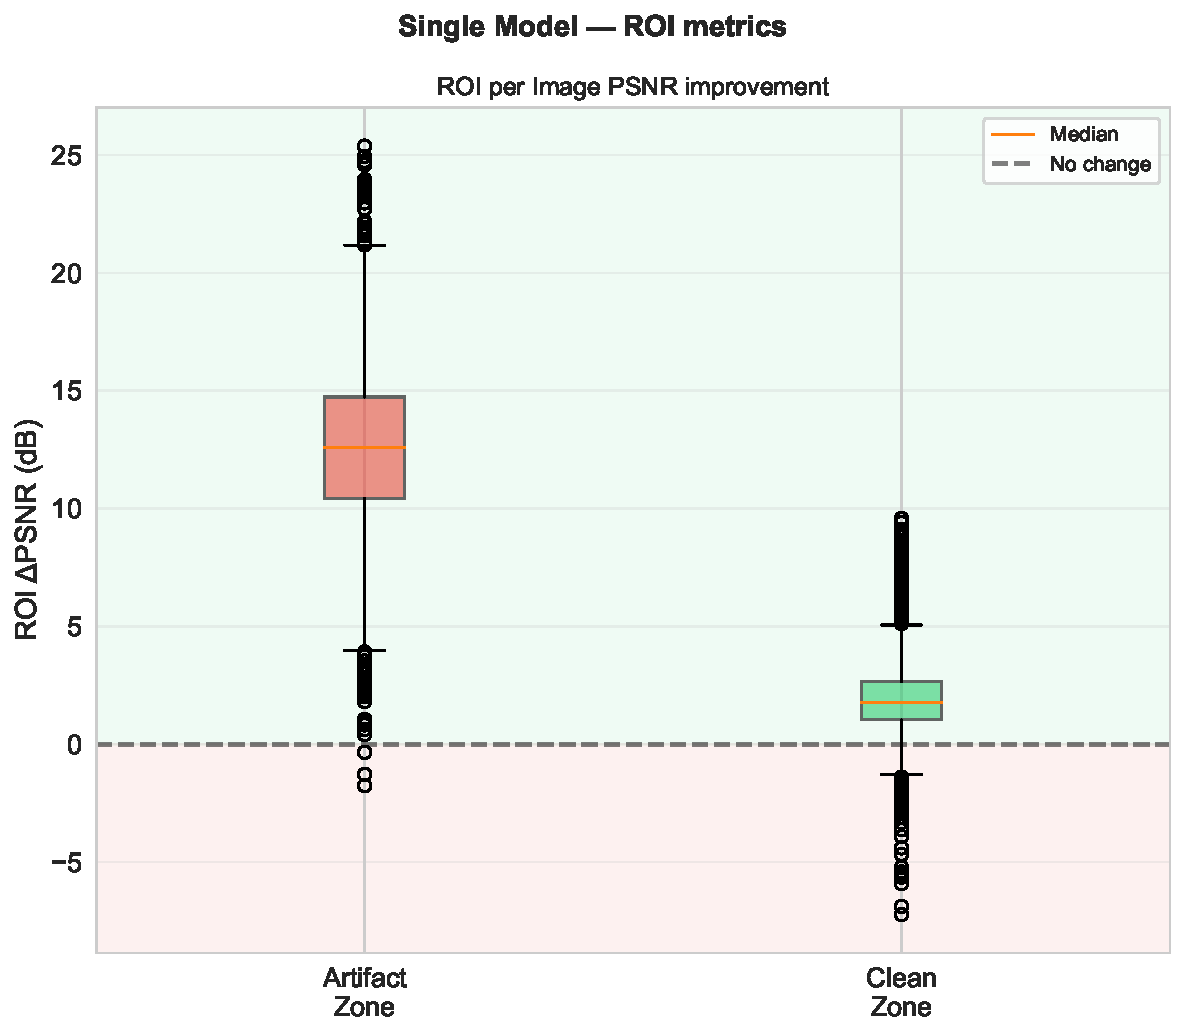
\includegraphics[width=0.84\linewidth]{Figures/Generated/evaluation_final/ROI/boxplot_roi_delta_psnr.pdf}
\end{figure}

\begin{figure}[H]
    \centering
    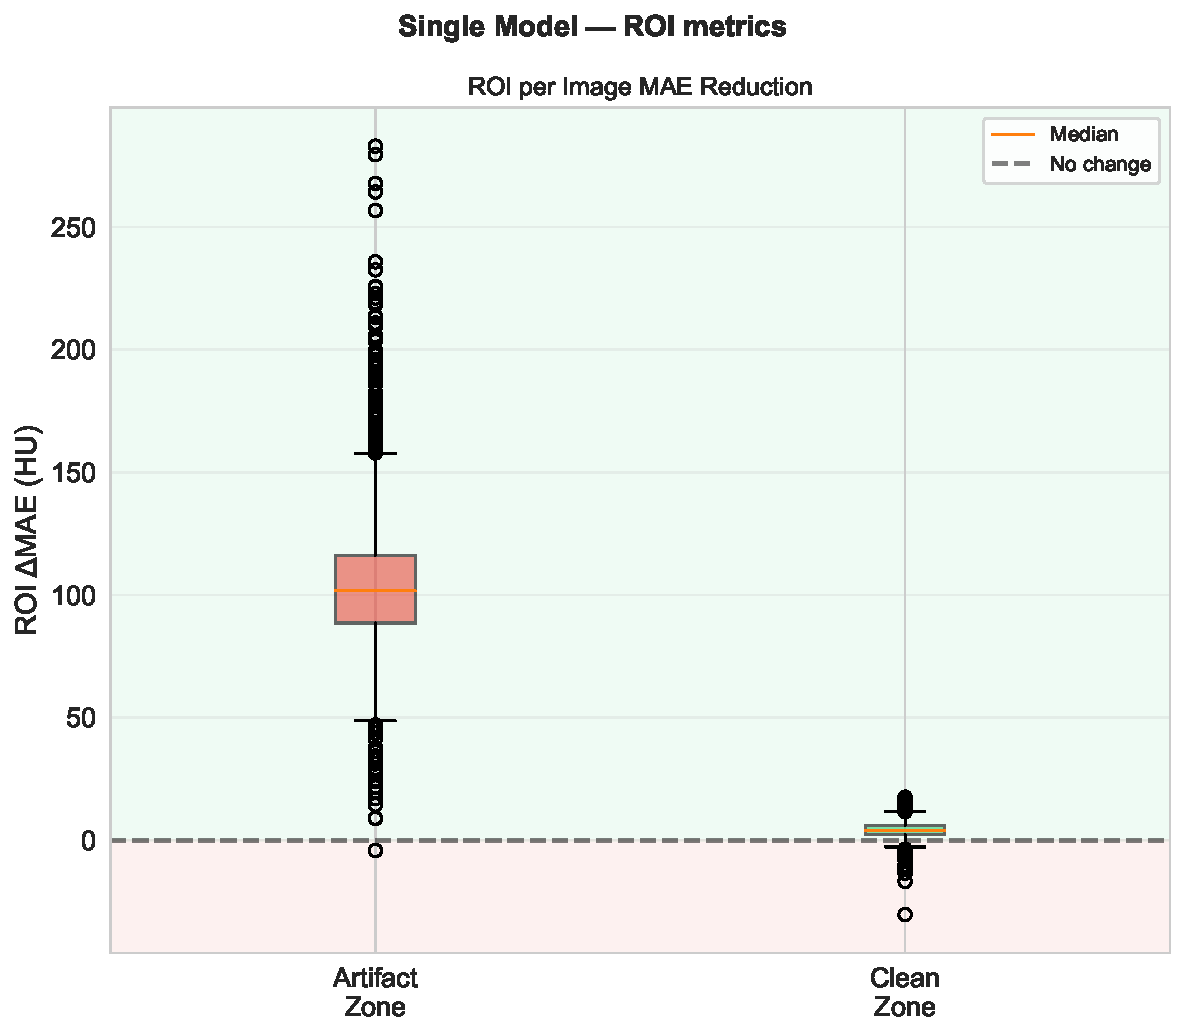
\includegraphics[width=0.84\linewidth]{Figures/Generated/evaluation_final/ROI/boxplot_roi_delta_mae.pdf}
\end{figure}
\captionsetup{skip=1.5pt}
\graphiccaptionof[Per-image ROI metric improvements]{Per-image distributions of\acrshort{ssim},\acrshort{psnr}, and\acrshort{mae} changes in the artifact and clean zones for the Single Model, seed 2024.}
\label{fig:roi-boxplots}
\endgroup

\begingroup
\setlength{\intextsep}{4pt}
\begin{figure}[H]
    \centering
    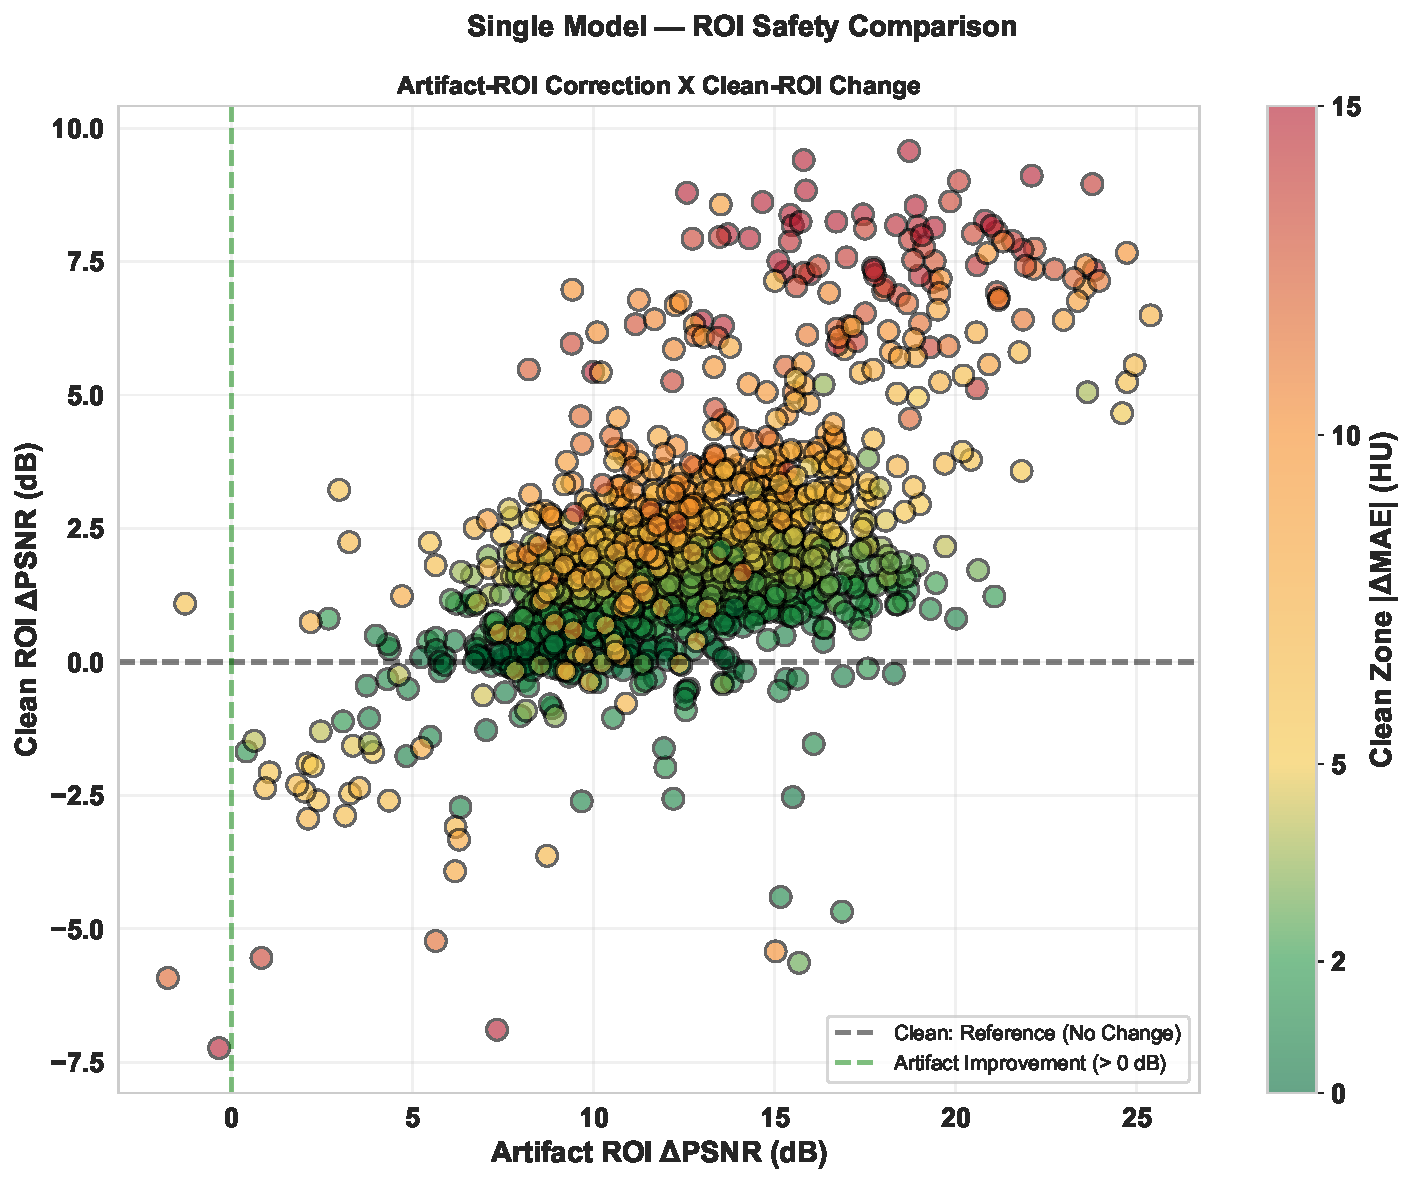
\includegraphics[width=0.84\linewidth]{Figures/Generated/evaluation_final/ROI/scatter_roi_safety.pdf}
\end{figure}

\begin{figure}[H]
    \centering
    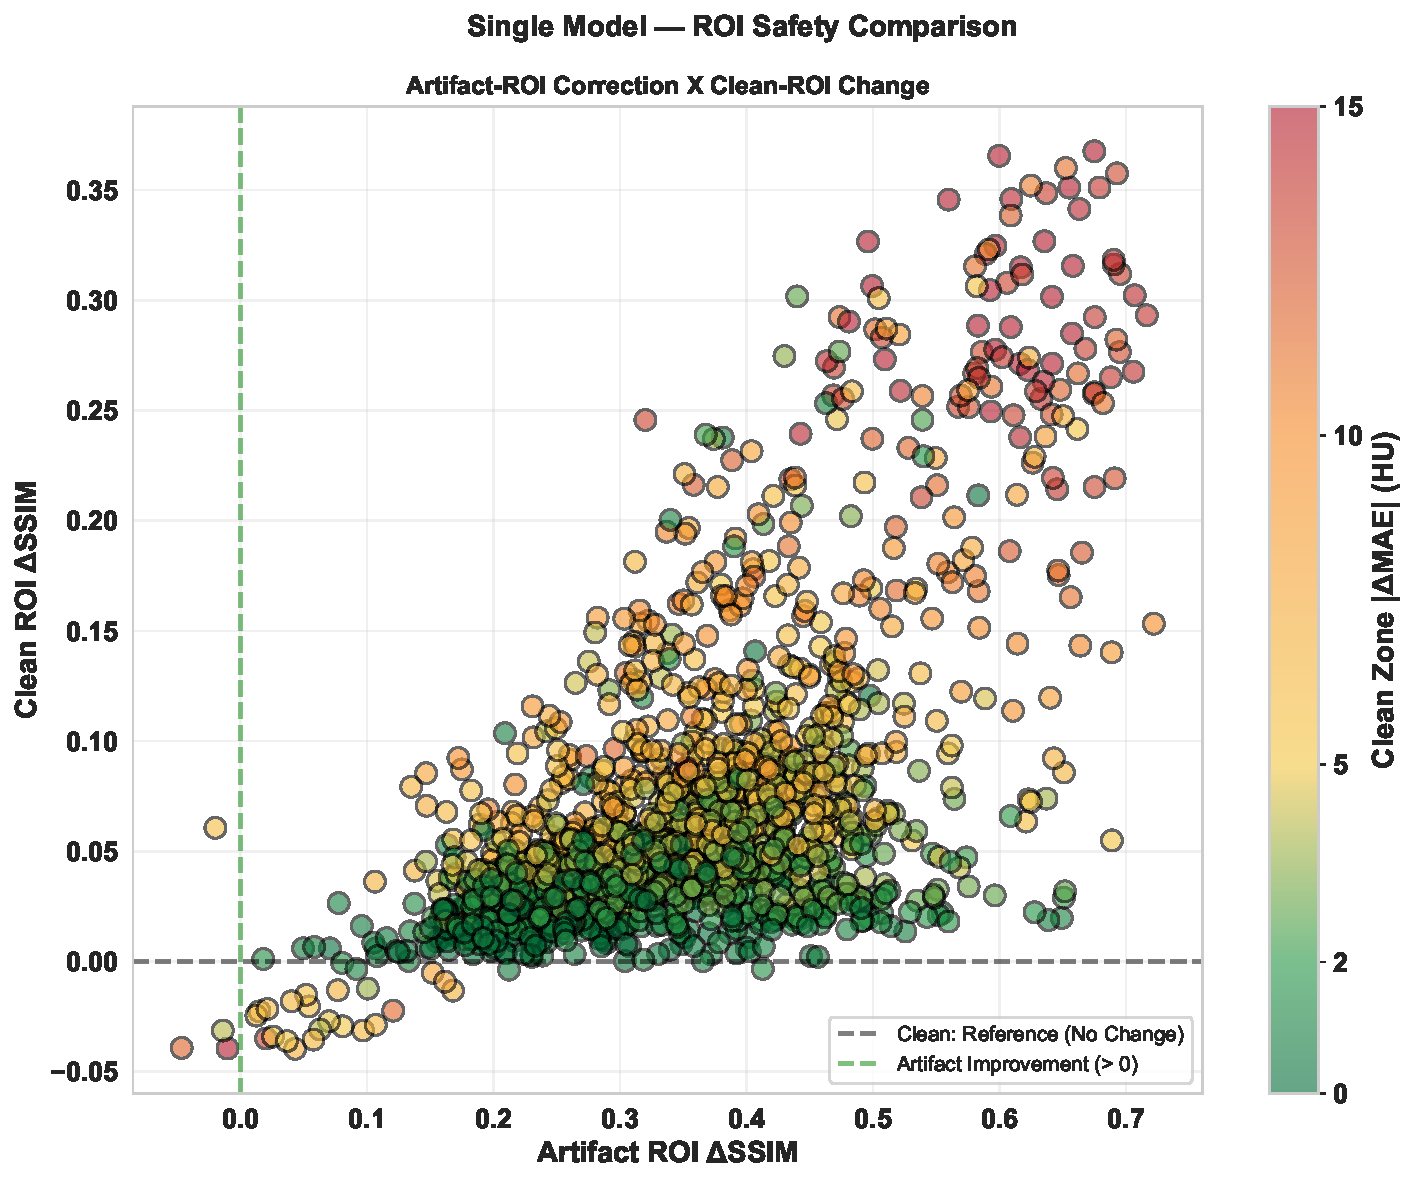
\includegraphics[width=0.84\linewidth]{Figures/Generated/evaluation_final/ROI/scatter_roi_safety_ssim.pdf}
\end{figure}
\captionsetup{skip=2pt}
\graphiccaptionof[Artifact-ROI correction versus clean-ROI change]{Per-image relationship between the\acrshort{ssim} \textbackslash\acrshort{psnr} improvement in the Artifact Zone and the\acrshort{ssim} \textbackslash\acrshort{psnr} change in the Clean Zone for the Single Model, seed 2024. Color encodes Clean Zone $|\Delta\mathrm{MAE}|$ in HU: green at 0--2 HU, yellow around 5 HU, orange around 10 HU, and red at or above 15 HU. Both plots use the same 0--15 HU scale, with values above 15 HU saturated in red. These color anchors are descriptive, not clinical thresholds.}
\label{fig:roi-safety}
\endgroup

\subsection{Global Outcomes}
\label{sec:global-outcomes}

Having established the Single Model, seed 2024, as the run selected for external evaluation, this subsection reports the global metrics, computed over all body-mask pixels without\acrshort{roi} stratification, as complementary evidence of overall reconstruction quality. They were not part of the basis for the selection decision above.

The \autoref{tab:global-ssim}, \autoref{tab:global-psnr}, and \autoref{tab:global-mae} present the slice-wise means. Since all runs were evaluated on the same test partition, the input value is common to both models for each seed. Across runs, reconstruction improved global structural similarity and radiometric fidelity relative to the corrupted input.

\begin{table}[htbp]
    \centering
    
    \begin{tabular}{cccc}
        \multicolumn{4}{c}{\textbf{SSIM global}} \\[4pt]
        \hline
        \textbf{Seed} & \textbf{Input} & \textbf{Single Model} & \textbf{Dual Model} \\
        \hline
        42   & $0.8361 \pm 0.0880$ & $0.9439 \pm 0.0289$ & $0.9424 \pm 0.0292$ \\
        1337 & $0.8361 \pm 0.0880$ & $0.9441 \pm 0.0286$ & $0.9421 \pm 0.0289$ \\
        2024 & $0.8361 \pm 0.0880$ & $0.9442 \pm 0.0288$ & $0.9432 \pm 0.0292$ \\
        \hline
    \end{tabular}
    \captionsetup{skip=2pt}
    \caption[Per-slice global SSIM on the test set]{Global\acrshort{ssim} per slice in test subset ($n=1478$), expressed as mean $\pm$ standard deviation.\tablecaptionnote{All input and model values are computed against the clean reference (\textit{ground truth}).}}
    \label{tab:global-ssim}
\end{table}

\begin{table}[htbp]
    \centering
    \begin{tabular}{cccc}
        \multicolumn{4}{c}{\textbf{PSNR global (dB)}} \\[4pt]
        \hline
        \textbf{Seed} & \textbf{Input} & \textbf{Single Model} & \textbf{Dual Model} \\
        \hline
        42   & $27.39 \pm 4.14$ & $35.09 \pm 2.82$ & $35.06 \pm 2.84$ \\
        1337 & $27.39 \pm 4.14$ & $35.13 \pm 2.81$ & $34.95 \pm 2.82$ \\
        2024 & $27.39 \pm 4.14$ & $35.20 \pm 2.84$ & $35.16 \pm 2.82$ \\
        \hline
    \end{tabular}
    \captionsetup{skip=2pt}
    \caption[Per-slice global\acrshort{psnr} on the test set]{Global\acrshort{psnr} per slice in test subset ($n=1478$), expressed as mean $\pm$ standard deviation.\tablecaptionnote{All input and model values are computed against the clean reference (\textit{ground truth}).}}
    \label{tab:global-psnr}
\end{table}

\begin{table}[htbp]
    \centering
    \begin{tabular}{cccc}
        \multicolumn{4}{c}{\textbf{MAE global (HU)}} \\[4pt]
        \hline
        \textbf{Seed} & \textbf{Input} & \textbf{Single Model} & \textbf{Dual Model} \\
        \hline
        42   & $36.569 \pm 21.906$ & $17.649 \pm 5.689$ & $17.654 \pm 5.905$ \\
        1337 & $36.569 \pm 21.906$ & $17.485 \pm 5.624$ & $17.842 \pm 5.789$ \\
        2024 & $36.569 \pm 21.906$ & $17.341 \pm 5.573$ & $17.475 \pm 5.563$ \\
        \hline
    \end{tabular}
    \captionsetup{skip=2pt}
    \caption[Per-slice global MAE on the test set]{Global\acrshort{mae} per slice in test subset ($n=1478$), expressed as mean $\pm$ standard deviation.\tablecaptionnote{All input and model values are computed against the clean reference (\textit{ground truth}).}}
    \label{tab:global-mae}
\end{table}
\FloatBarrier
The seed-wise global tables show that the Single Model, seed 2024, was not an isolated run: the three Single Model runs had very similar global performance. Seed 2024 was at the favorable extreme for global\acrshort{ssim},\acrshort{psnr}, and\acrshort{mae}.

The patient-level deltas and their confidence intervals are shown in \autoref{tab:delta-ssim-paciente}, \autoref{tab:delta-psnr-paciente}, and \autoref{tab:delta-mae-paciente}. All six runs showed positive mean improvement for the three global metrics, and the corresponding confidence intervals excluded the null value.
\begin{table}[htbp]
    \centering
    \begin{tabular}{ccc}
        \multicolumn{3}{c}{\textbf{$\Delta$SSIM Global (95\% CI)}} \\[4pt]
        \hline
        \textbf{Seed} & \textbf{Single Model} & \textbf{Dual Model} \\
        \hline
        42   & 0.0887 [0.0728; 0.1063] & 0.0870 [0.0713; 0.1043] \\
        1337 & 0.0891 [0.0734; 0.1065] & 0.0867 [0.0710; 0.1041] \\
        2024 & 0.0891 [0.0732; 0.1066] & 0.0879 [0.0719; 0.1053] \\
        \hline
    \end{tabular}
    \captionsetup{skip=2pt}
    \caption[Patient-level global $\Delta$SSIM]{$\Delta\acrshort{ssim}$ global aggregated per patient in the test subset ($n=41$). CI: 95\% confidence interval.\tablecaptionnote{$\Delta\mathrm{SSIM}=\mathrm{SSIM}(\mathrm{Model},\mathrm{GT})-\mathrm{SSIM}(\mathrm{Input},\mathrm{GT})$.}}
    \label{tab:delta-ssim-paciente}
\end{table}

\begin{table}[htbp]
    \centering
    \begin{tabular}{ccc}
        \multicolumn{3}{c}{\textbf{$\Delta$PSNR Global (dB, 95\% CI)}} \\[4pt]
        \hline
        \textbf{Seed} & \textbf{Single Model} & \textbf{Dual Model} \\
        \hline
        42   & 6.96 [6.22; 7.68] & 6.96 [6.24; 7.65] \\
        1337 & 7.05 [6.33; 7.75] & 6.85 [6.12; 7.55] \\
        2024 & 7.11 [6.36; 7.83] & 7.06 [6.31; 7.78] \\
        \hline
    \end{tabular}
    \captionsetup{skip=2pt}
    \caption[Patient-level global $\Delta$PSNR]{$\Delta\acrshort{psnr}$ global aggregated per patient in the test subset ($n=41$). CI: 95\% confidence interval.\tablecaptionnote{$\Delta\mathrm{PSNR}=\mathrm{PSNR}(\mathrm{Model},\mathrm{GT})-\mathrm{PSNR}(\mathrm{Input},\mathrm{GT})$.}}
    \label{tab:delta-psnr-paciente}
\end{table}

\begin{table}[htbp]
    \centering
    \begin{tabular}{ccc}
        \multicolumn{3}{c}{\textbf{$\Delta$MAE Global (HU, 95\% CI)}} \\[4pt]
        \hline
        \textbf{Seed} & \textbf{Single Model} & \textbf{Dual Model} \\
        \hline
        42   & 15.3 [12.2; 19.0] & 15.3 [12.3; 18.9] \\
        1337 & 15.6 [12.4; 19.3] & 15.2 [12.1; 18.8] \\
        2024 & 15.7 [12.5; 19.5] & 15.5 [12.4; 19.3] \\
        \hline
    \end{tabular}
    \captionsetup{skip=2pt}
    \caption[Patient-level global $\Delta$MAE]{$\Delta\acrshort{mae}$ global aggregated per patient in the test subset ($n=41$). Values $>0$ indicate improvement. CI: 95\% confidence interval.\tablecaptionnote{$\Delta\mathrm{MAE}=\mathrm{MAE}(\mathrm{Input},\mathrm{GT})-\mathrm{MAE}(\mathrm{Model},\mathrm{GT})$. Positive values indicate error reduction.}}
    \label{tab:delta-mae-paciente}
\end{table}
\FloatBarrier

For the selected run, the histograms in \autoref{fig:global-improvement-histograms} show the per-slice distribution of global changes. They make the uncommon unfavorable cases visible, while statistical inference remains based on the patient-level summaries in the preceding tables.
\begingroup
\setlength{\intextsep}{4pt}
\begin{figure}[H]
    \centering
    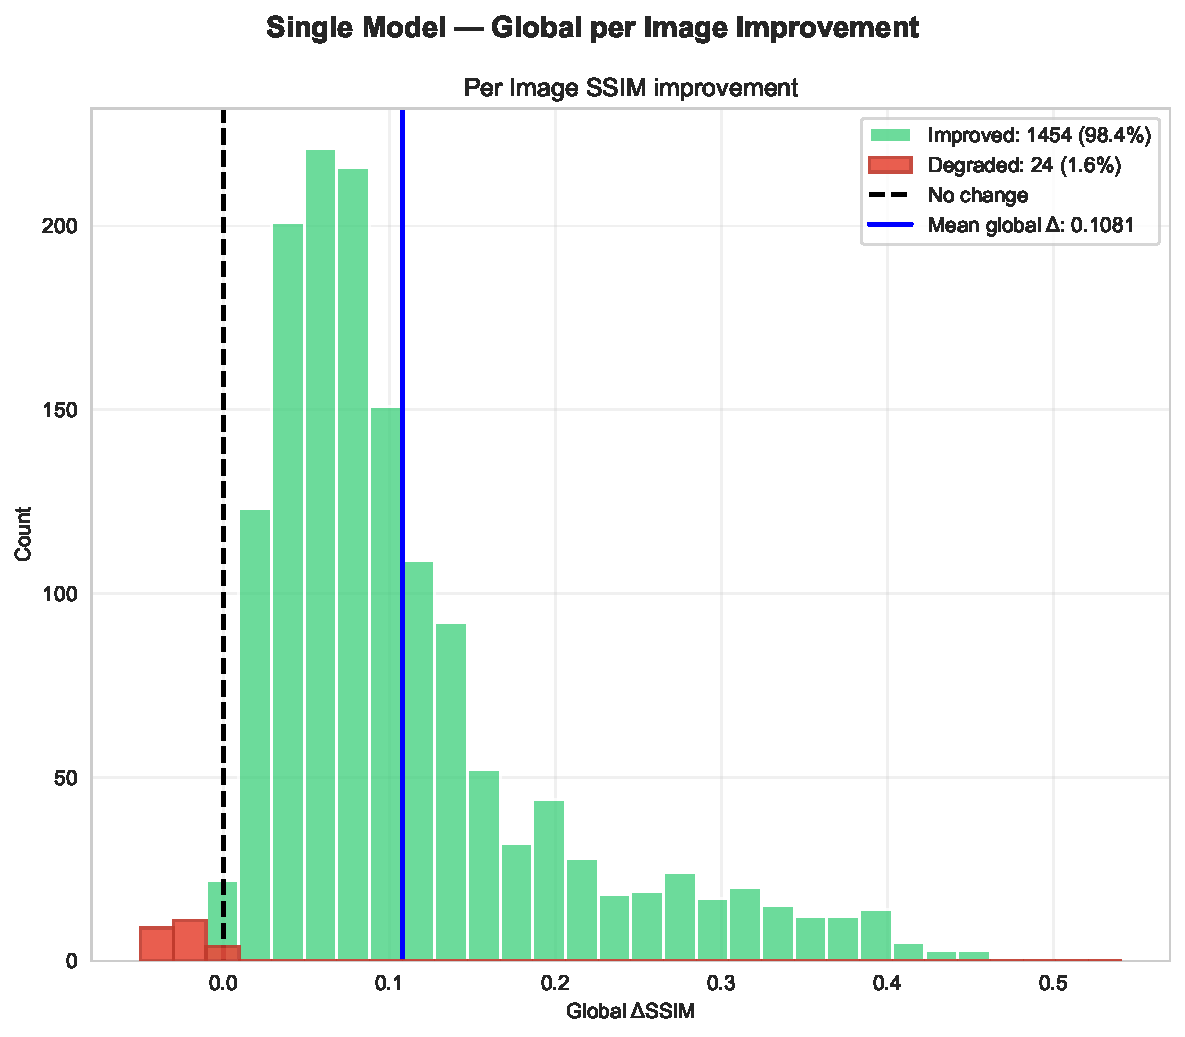
\includegraphics[width=0.83\linewidth]{Figures/Generated/evaluation_final/Global/histogram_global_delta_ssim.pdf}
\end{figure}

\begin{figure}[H]
    \centering
    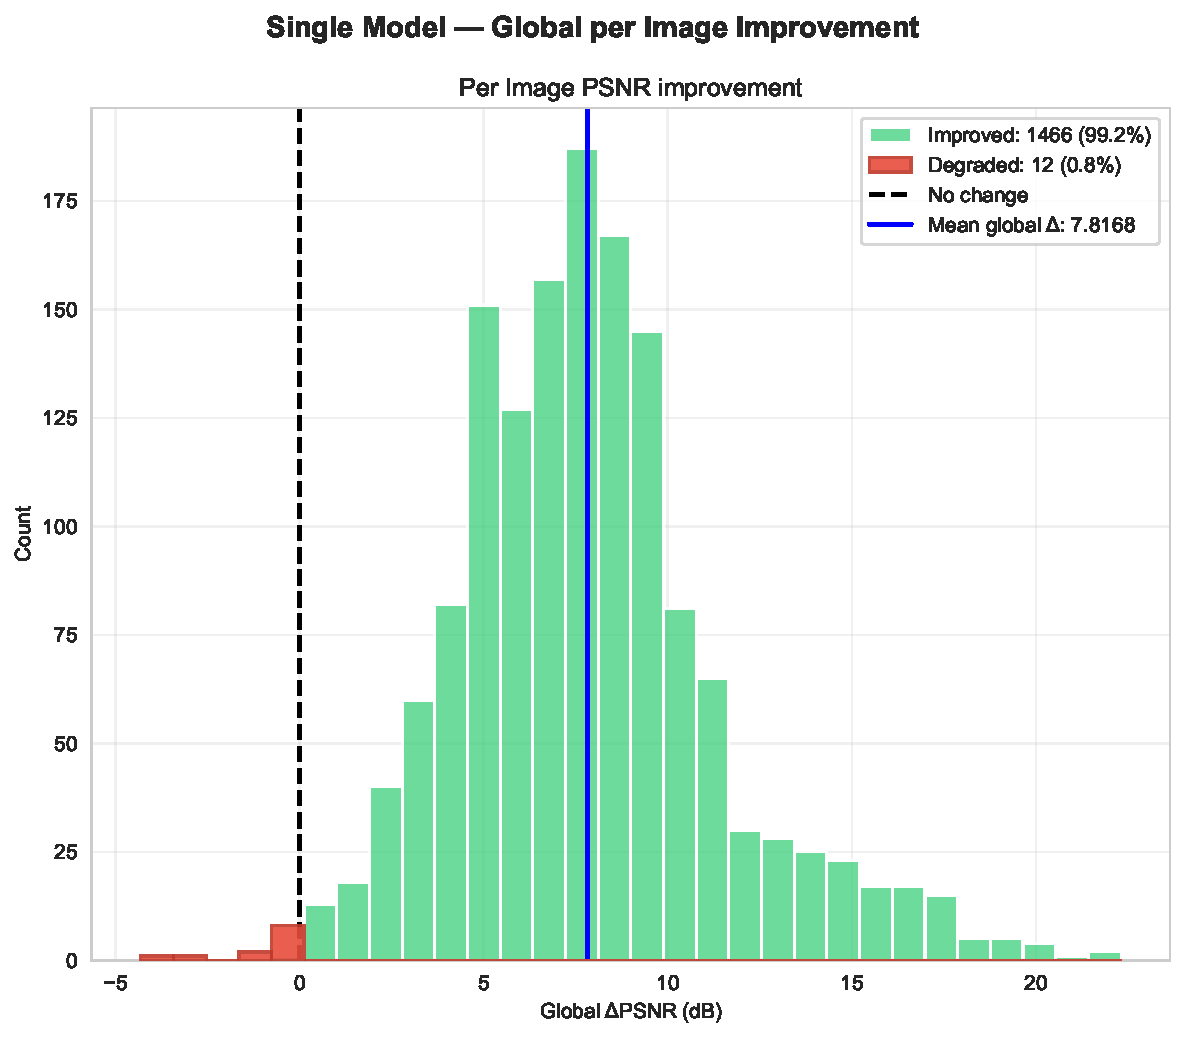
\includegraphics[width=0.84\linewidth]{Figures/Generated/evaluation_final/Global/histogram_global_delta_psnr.pdf}

\captionsetup{skip=1.5pt}
\graphiccaptionof[Per-image global PSNR and SSIM improvement]{Per-image global improvement over the corrupted input for the Single Model, seed 2024: $\Delta$SSIM (top) and $\Delta$PSNR (bottom).}
\end{figure}
\label{fig:global-improvement-histograms}
\endgroup
\FloatBarrier

As an additional descriptive check of overall\acrshort{hu} calibration, \autoref{fig:bland-altman-patient-hu} presents patient-level agreement between the reconstruction and the clean reference. It indicates a small positive shift in global mean intensity, but does not quantify local artifact removal or replace the global and\acrshort{roi} metrics.

\begin{figure}[htbp]
    \centering
    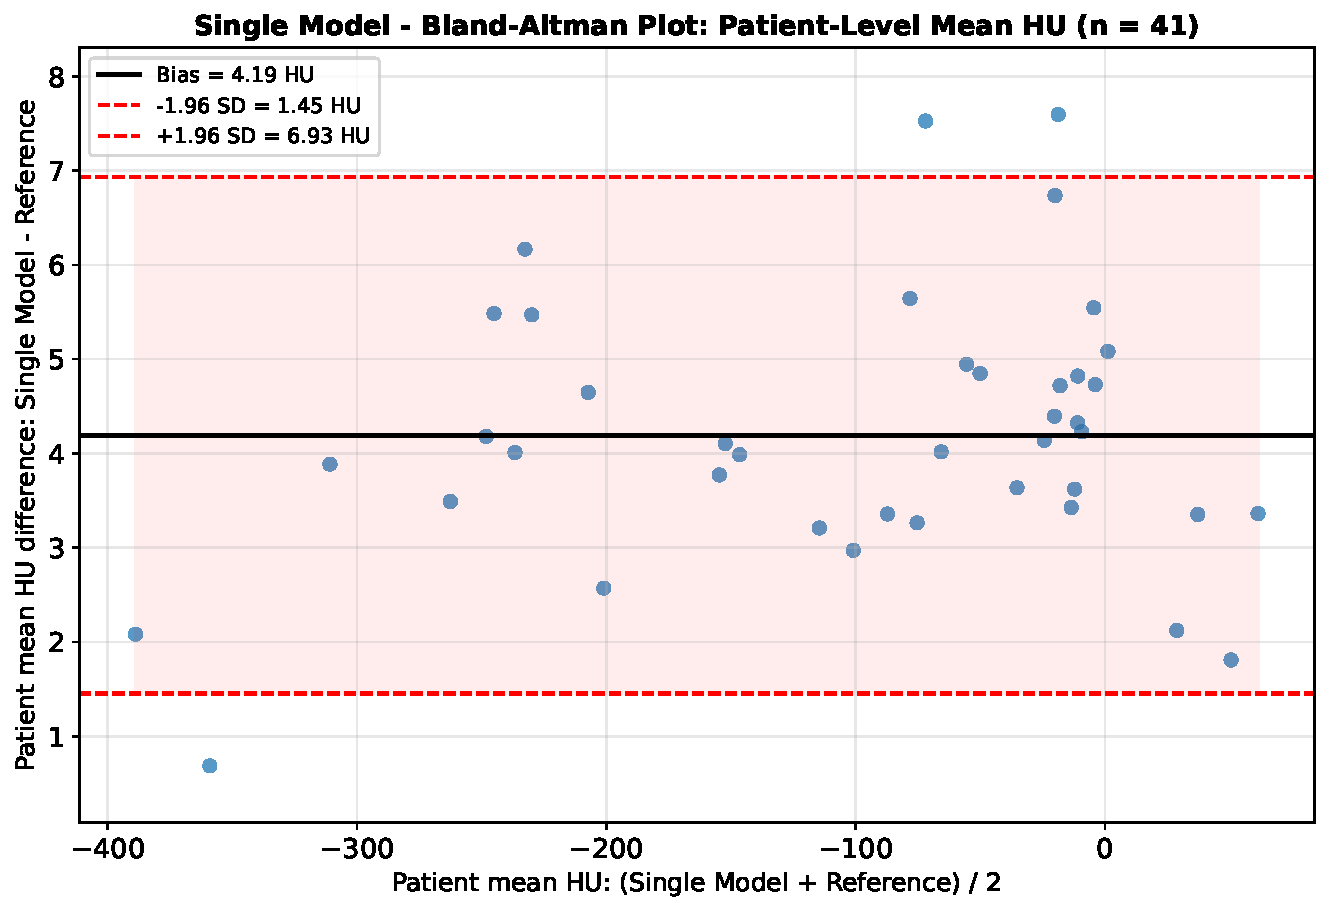
\includegraphics[width=0.84\linewidth]{Figures/Generated/evaluation_final/Global/bland_altman_patient_mean_hu.pdf}
    \captionsetup{skip=1.5pt}
    \graphiccaption[Patient-level Bland--Altman agreement of mean HU]{Bland--Altman agreement between the Single Model reconstruction and the clean reference for patient-level mean\acrshort{hu} ($n=41$). Each patient mean was calculated over all valid body-mask pixels. Positive differences indicate higher mean\acrshort{hu} in the reconstruction.}
    \label{fig:bland-altman-patient-hu}
\end{figure}
\FloatBarrier

\subsection{Residual Maps in Extreme Cases}
\label{sec:residual-maps-extremes}

To complement the results, six individual cases from the Single Model, seed 2024, were inspected in the test partition. The selection was made exclusively by the per-slice $\Delta\acrshort{ssim}$ in the Artifact Zone. The three highest values correspond to the greatest structural improvement in that region relative to the input, while the three lowest values correspond to the smallest structural improvement. Thus, the terms ``greatest'' and ``smallest'' improvement in this subsection refer only to this quantitative criterion.

In each map, the first row shows the correction required by the clean reference, the correction produced by the model, and the remaining residual error. The second row shows the absolute errors of the input and output and their difference, where green indicates error reduction and red indicates worsening. The yellow outline delimits the Artifact Zone. Color scales are adjusted individually for each slice to preserve detail; comparisons between cases should therefore prioritize spatial patterns and the panel summaries rather than apparent color intensity alone. Below each map, the corresponding artifact input, model output, and clean reference are shown.

\begin{figure}[!htbp]
\centering
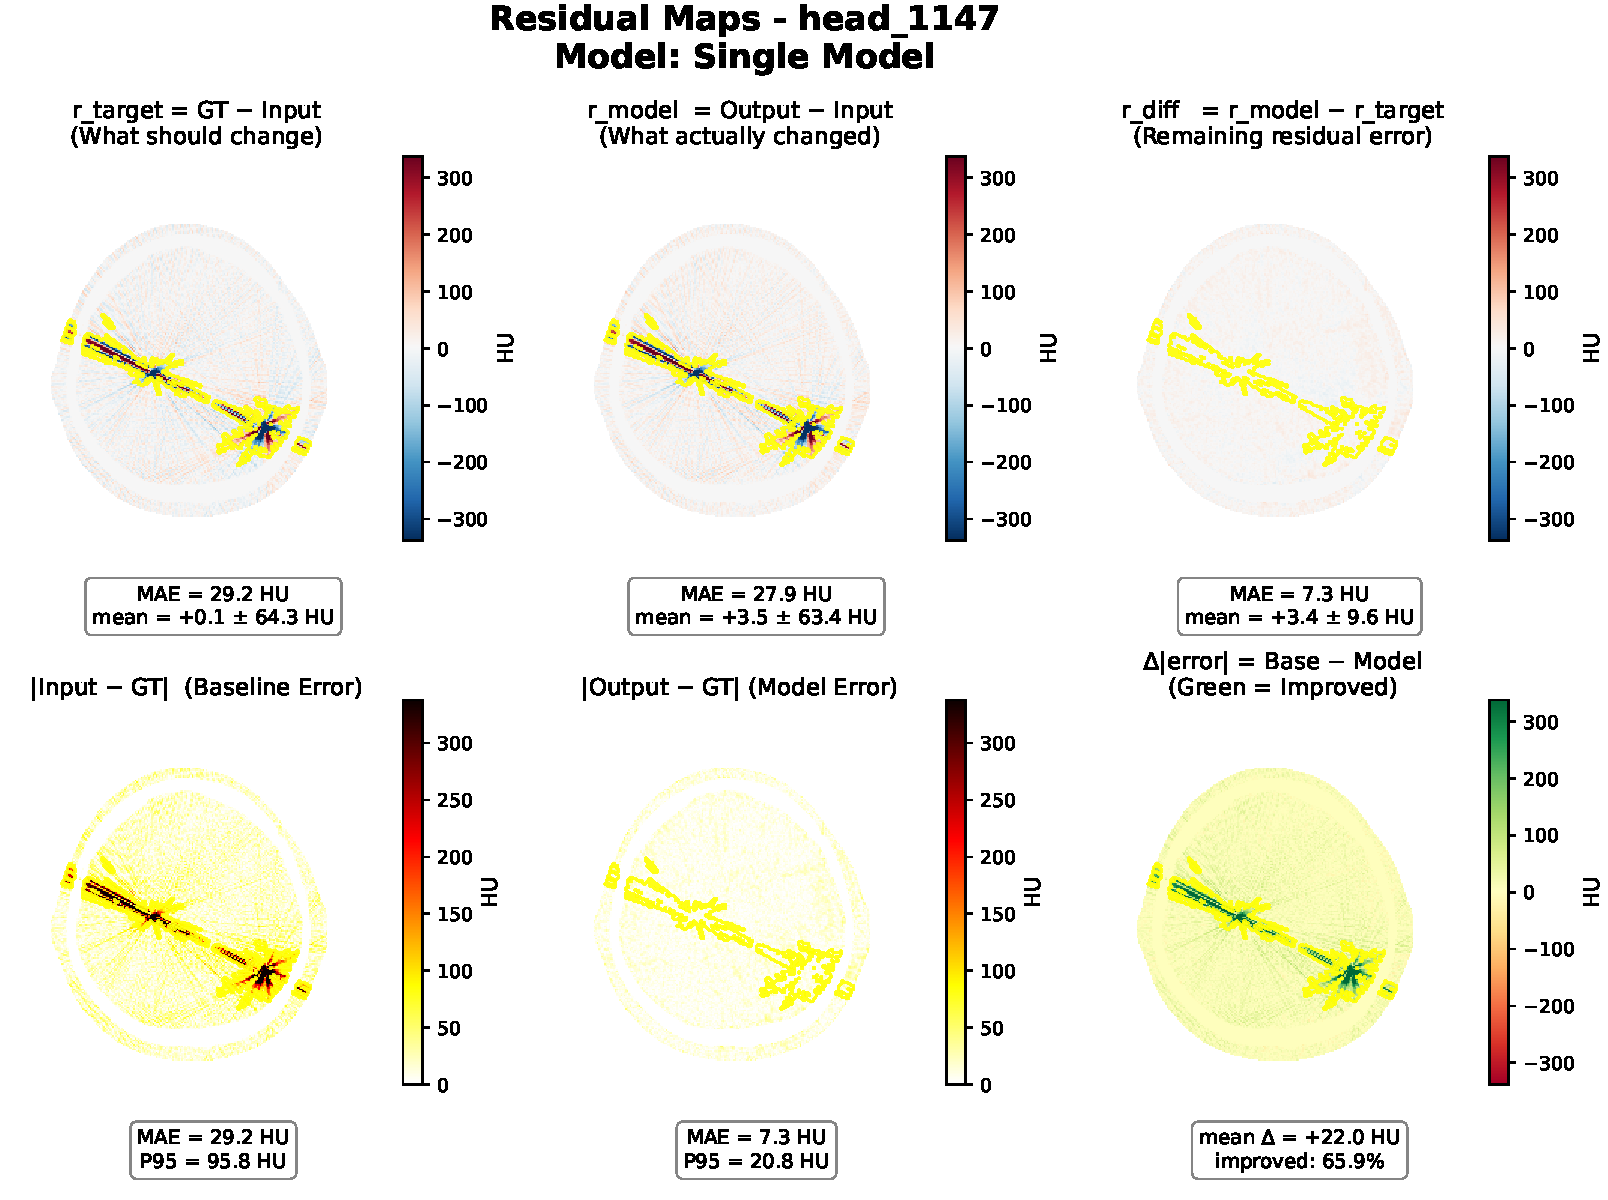
\includegraphics[width=\linewidth]{Figures/Generated/evaluation_final/Residuals/residual_greatest_structural_improvement_01_s1250.pdf}
\medskip
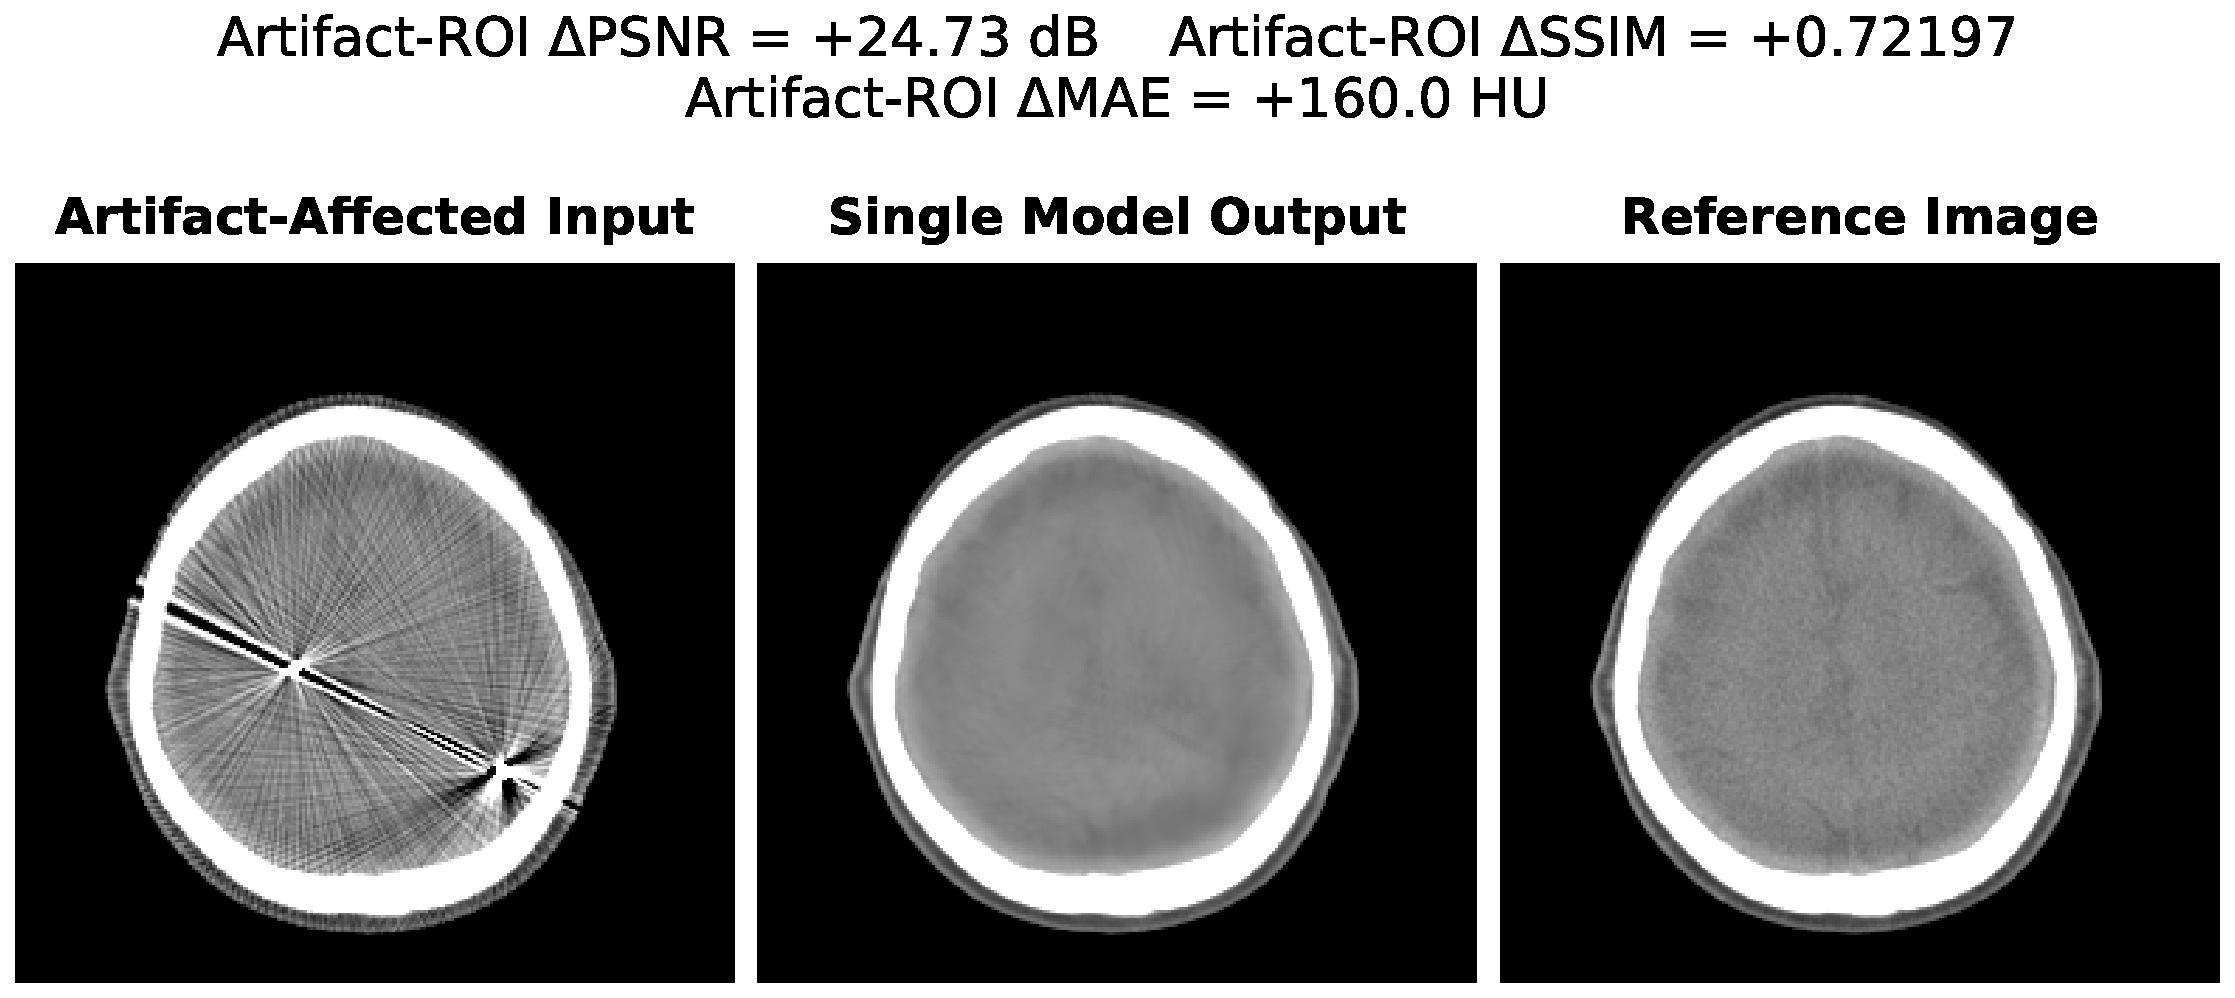
\includegraphics[width=0.94\linewidth]{Figures/Generated/evaluation_final/Residuals/visualization_greatest_structural_improvement_01_s1250.pdf}
\captionsetup{skip=2pt}
\caption[Greatest Artifact-ROI $\Delta$SSIM: head\_1147]{Residual map (top) and reconstruction visualization (bottom) for case head\_1147 (test-set index 1250), selected among the three highest artifact-ROI $\Delta$SSIM values ($\Delta\mathrm{SSIM}_{\mathrm{ROI}}=+0.7220$; global $\Delta\mathrm{SSIM}=+0.1649$; $\Delta\mathrm{PSNR}=+15.99$~dB). The yellow contour delimits the artifact ROI; all error maps are restricted to the body mask.}
\label{fig:residual-greatest-structural-improvement-1250}
\end{figure}

\begin{figure}[!htbp]
\centering
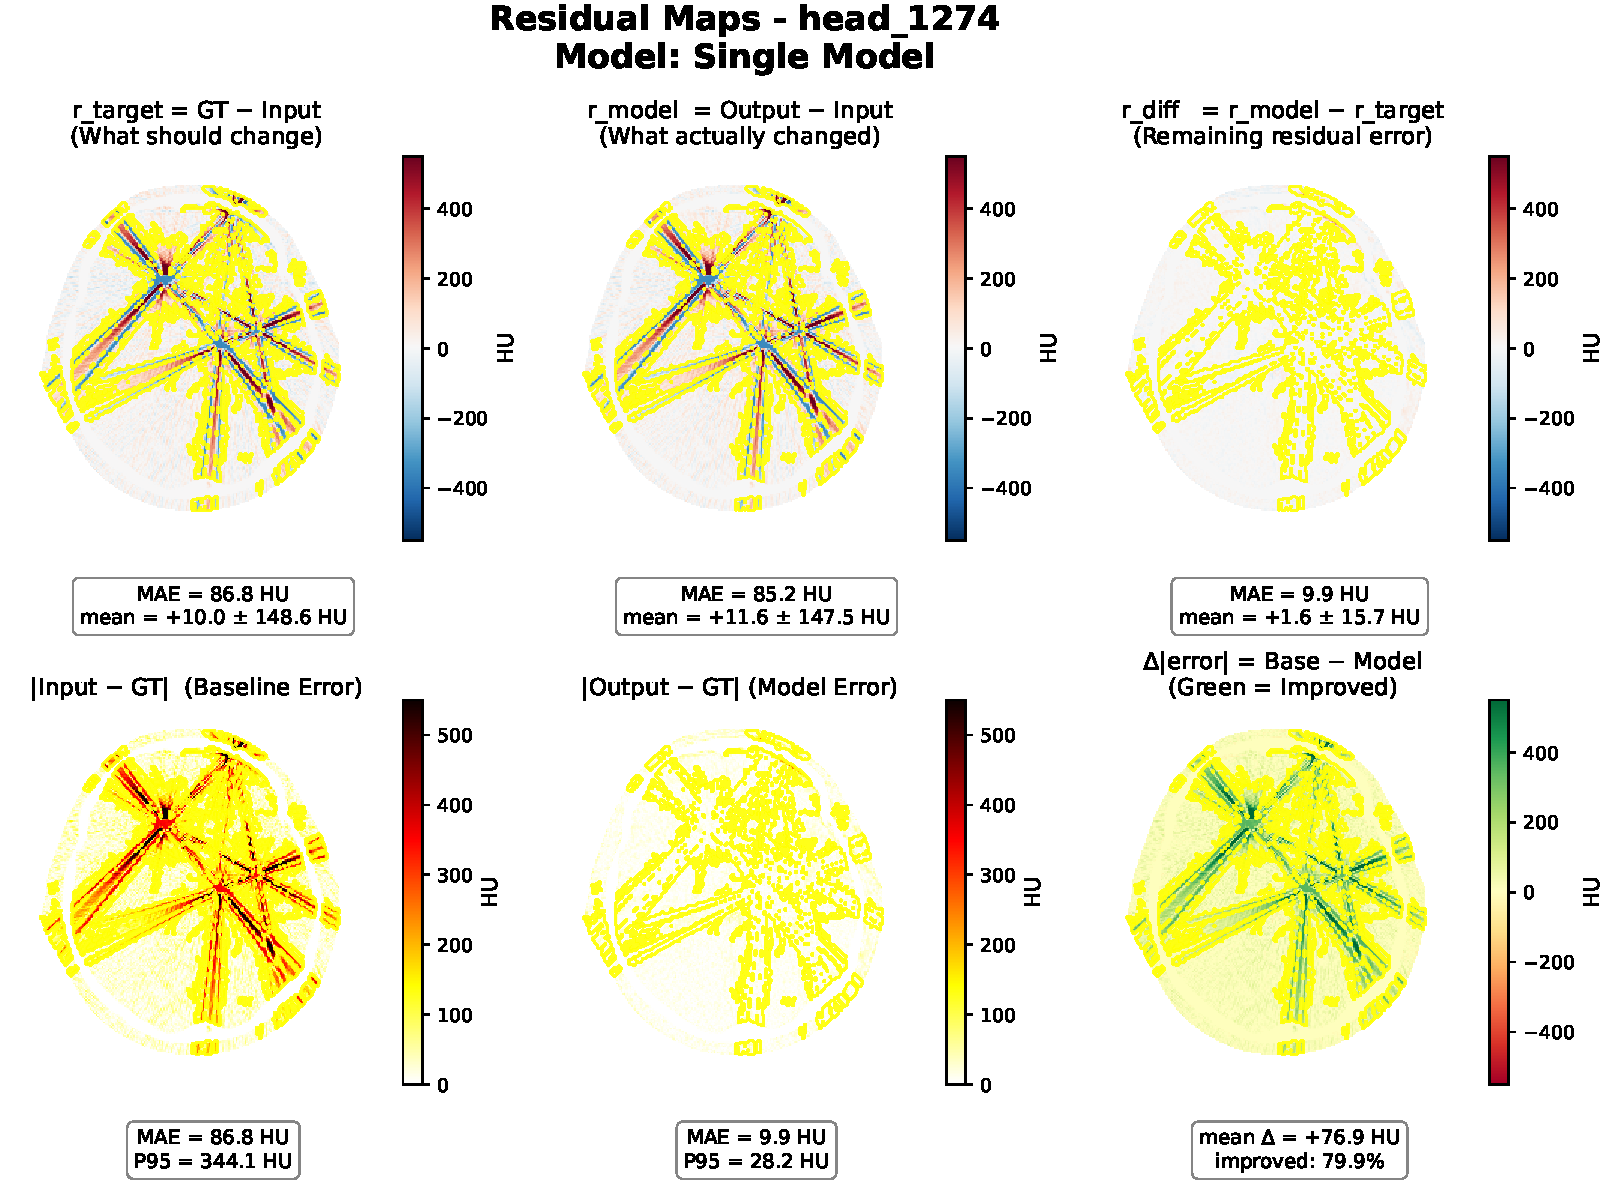
\includegraphics[width=\linewidth]{Figures/Generated/evaluation_final/Residuals/residual_greatest_structural_improvement_02_s1364.pdf}
\medskip
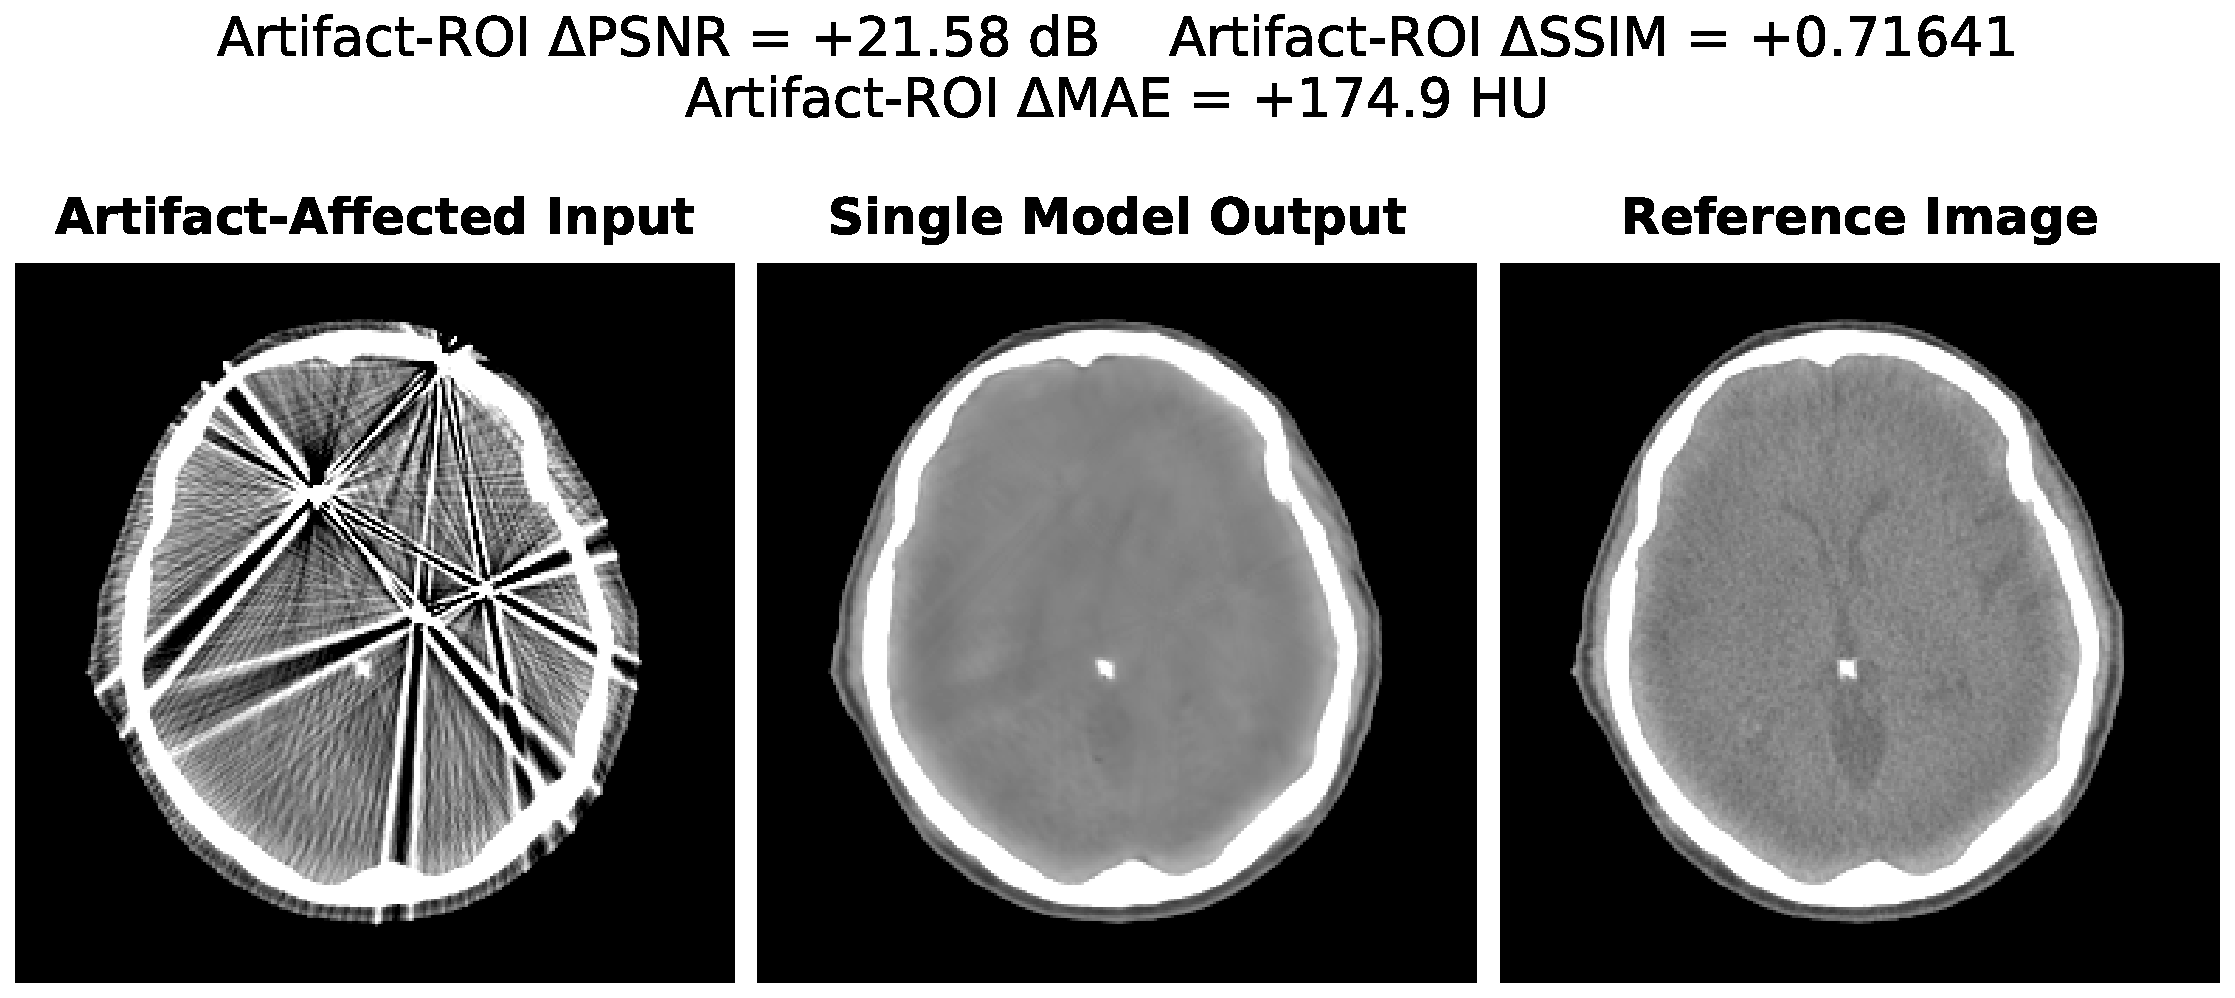
\includegraphics[width=0.94\linewidth]{Figures/Generated/evaluation_final/Residuals/visualization_greatest_structural_improvement_02_s1364.pdf}
\captionsetup{skip=2pt}
\caption[Greatest Artifact-ROI $\Delta$SSIM: head\_1274]{Residual map (top) and reconstruction visualization (bottom) for case head\_1274 (test-set index 1364), selected among the three highest artifact-ROI $\Delta$SSIM values ($\Delta\mathrm{SSIM}_{\mathrm{ROI}}=+0.7164$; global $\Delta\mathrm{SSIM}=+0.3752$; $\Delta\mathrm{PSNR}=+19.48$~dB). The yellow contour delimits the artifact ROI; all error maps are restricted to the body mask.}
\label{fig:residual-greatest-structural-improvement-1364}
\end{figure}

\begin{figure}[!htbp]
\centering
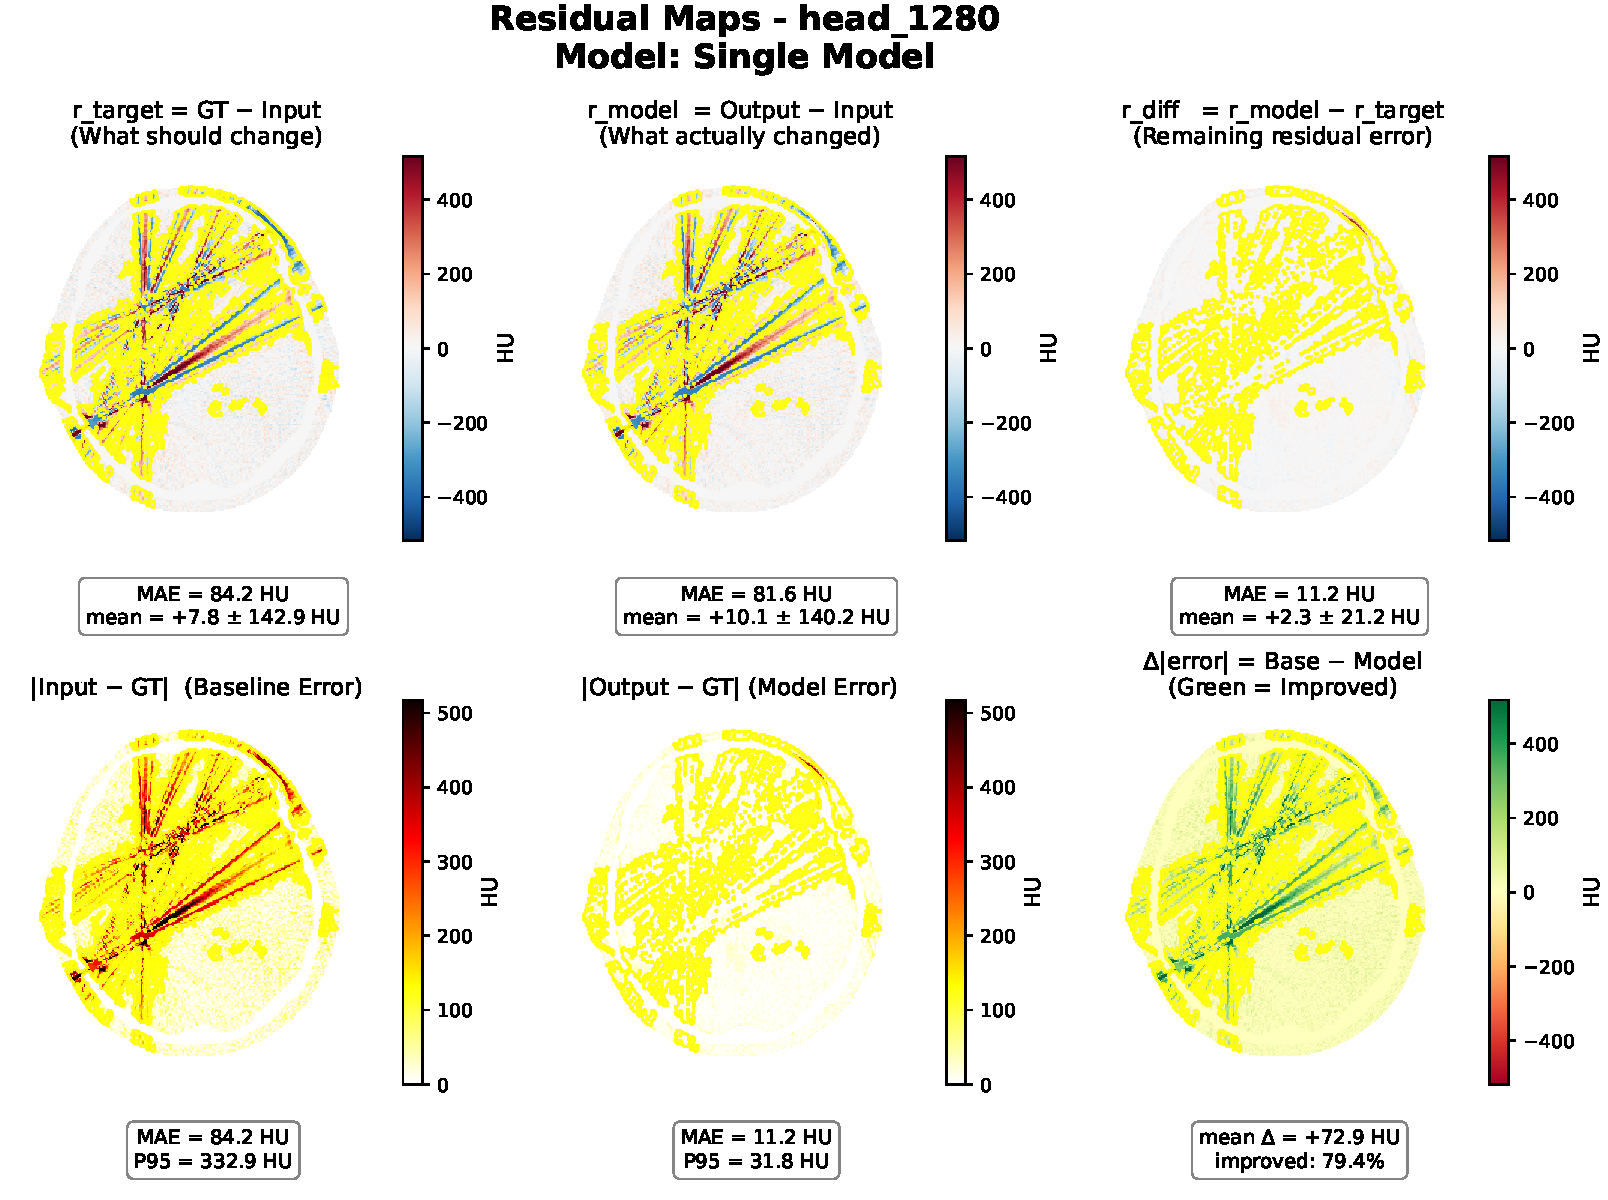
\includegraphics[width=\linewidth]{Figures/Generated/evaluation_final/Residuals/residual_greatest_structural_improvement_03_s1369.pdf}
\medskip
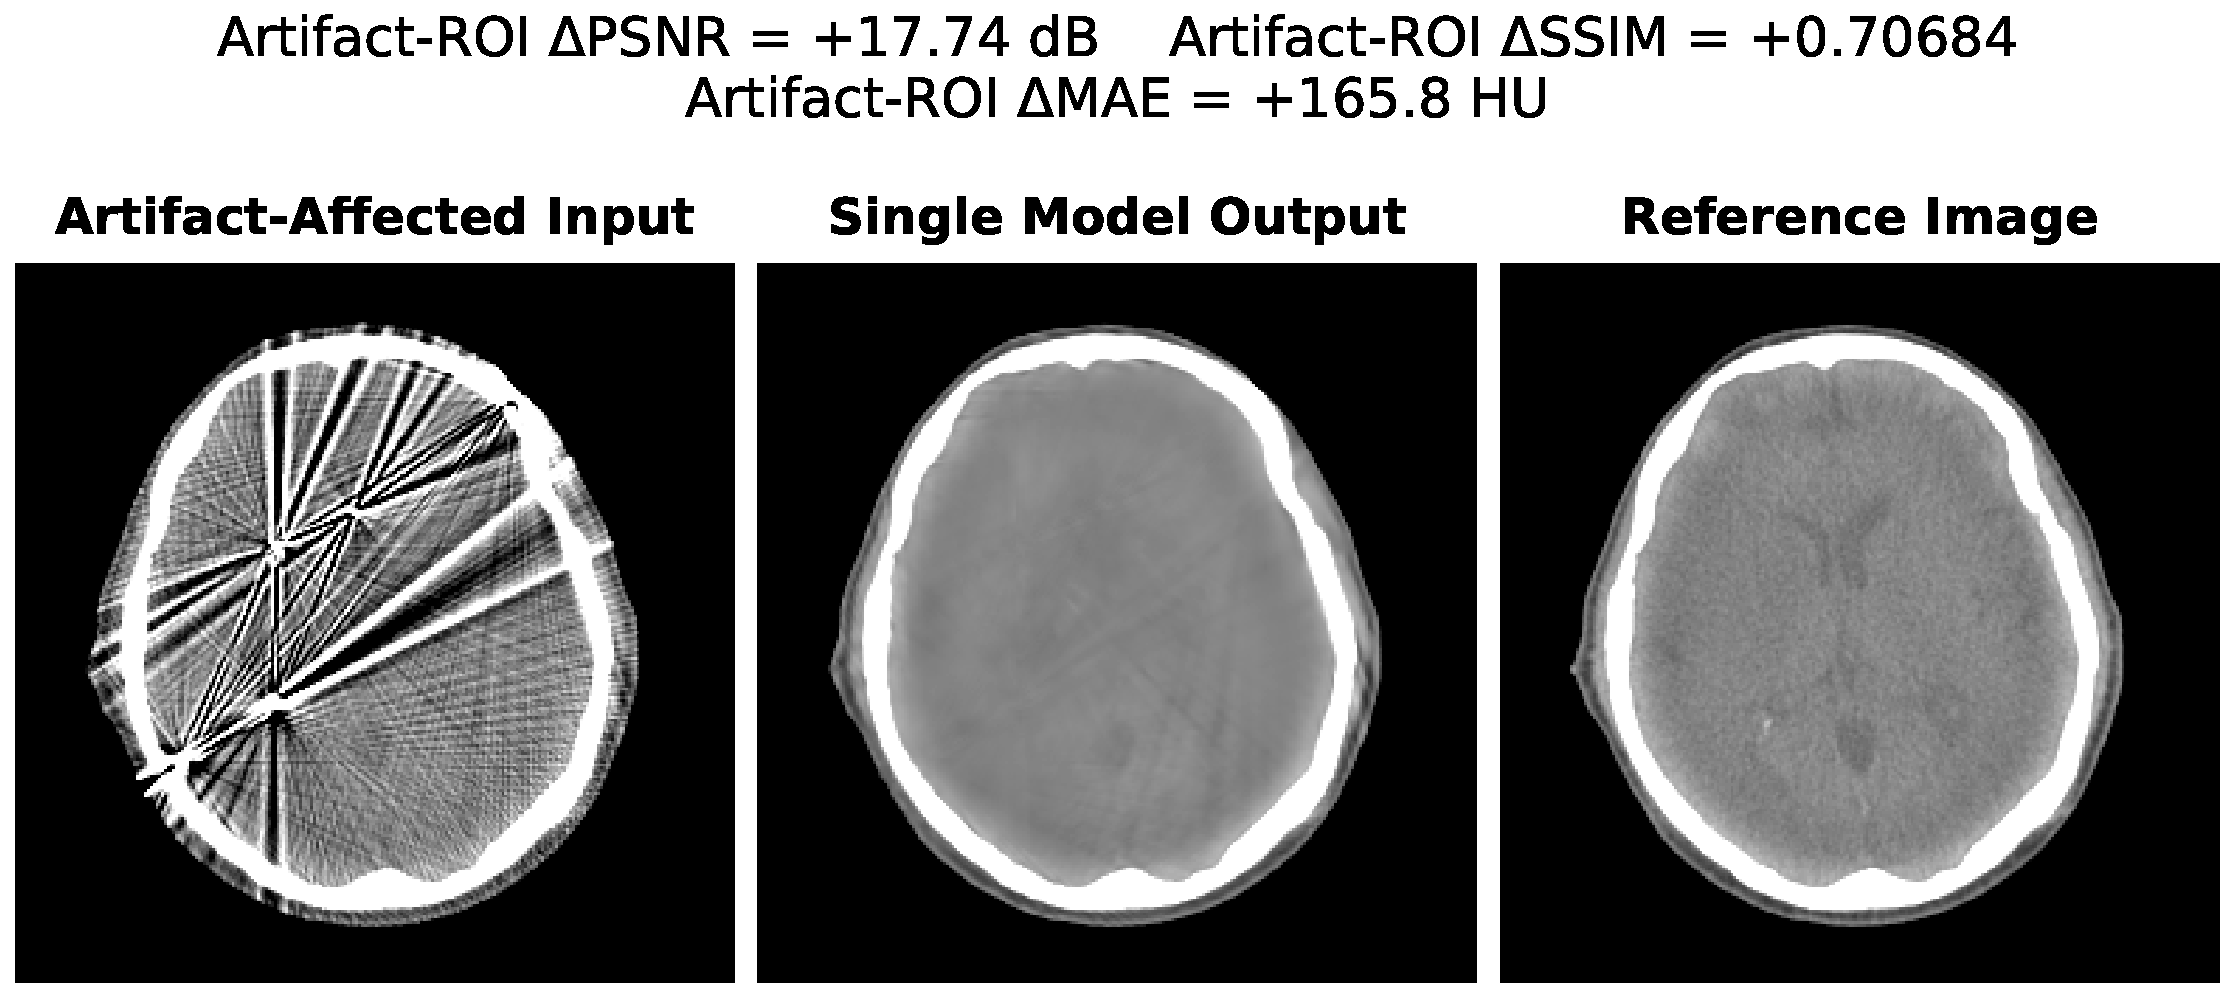
\includegraphics[width=0.94\linewidth]{Figures/Generated/evaluation_final/Residuals/visualization_greatest_structural_improvement_03_s1369.pdf}
\captionsetup{skip=2pt}
\caption[Greatest Artifact-ROI $\Delta$SSIM: head\_1280]{Residual map (top) and reconstruction visualization (bottom) for case head\_1280 (test-set index 1369), selected among the three highest artifact-ROI $\Delta$SSIM values ($\Delta\mathrm{SSIM}_{\mathrm{ROI}}=+0.7068$; global $\Delta\mathrm{SSIM}=+0.3837$; $\Delta\mathrm{PSNR}=+16.53$~dB). The yellow contour delimits the artifact ROI; all error maps are restricted to the body mask.}
\label{fig:residual-greatest-structural-improvement-1369}
\end{figure}

\begin{figure}[!htbp]
\centering
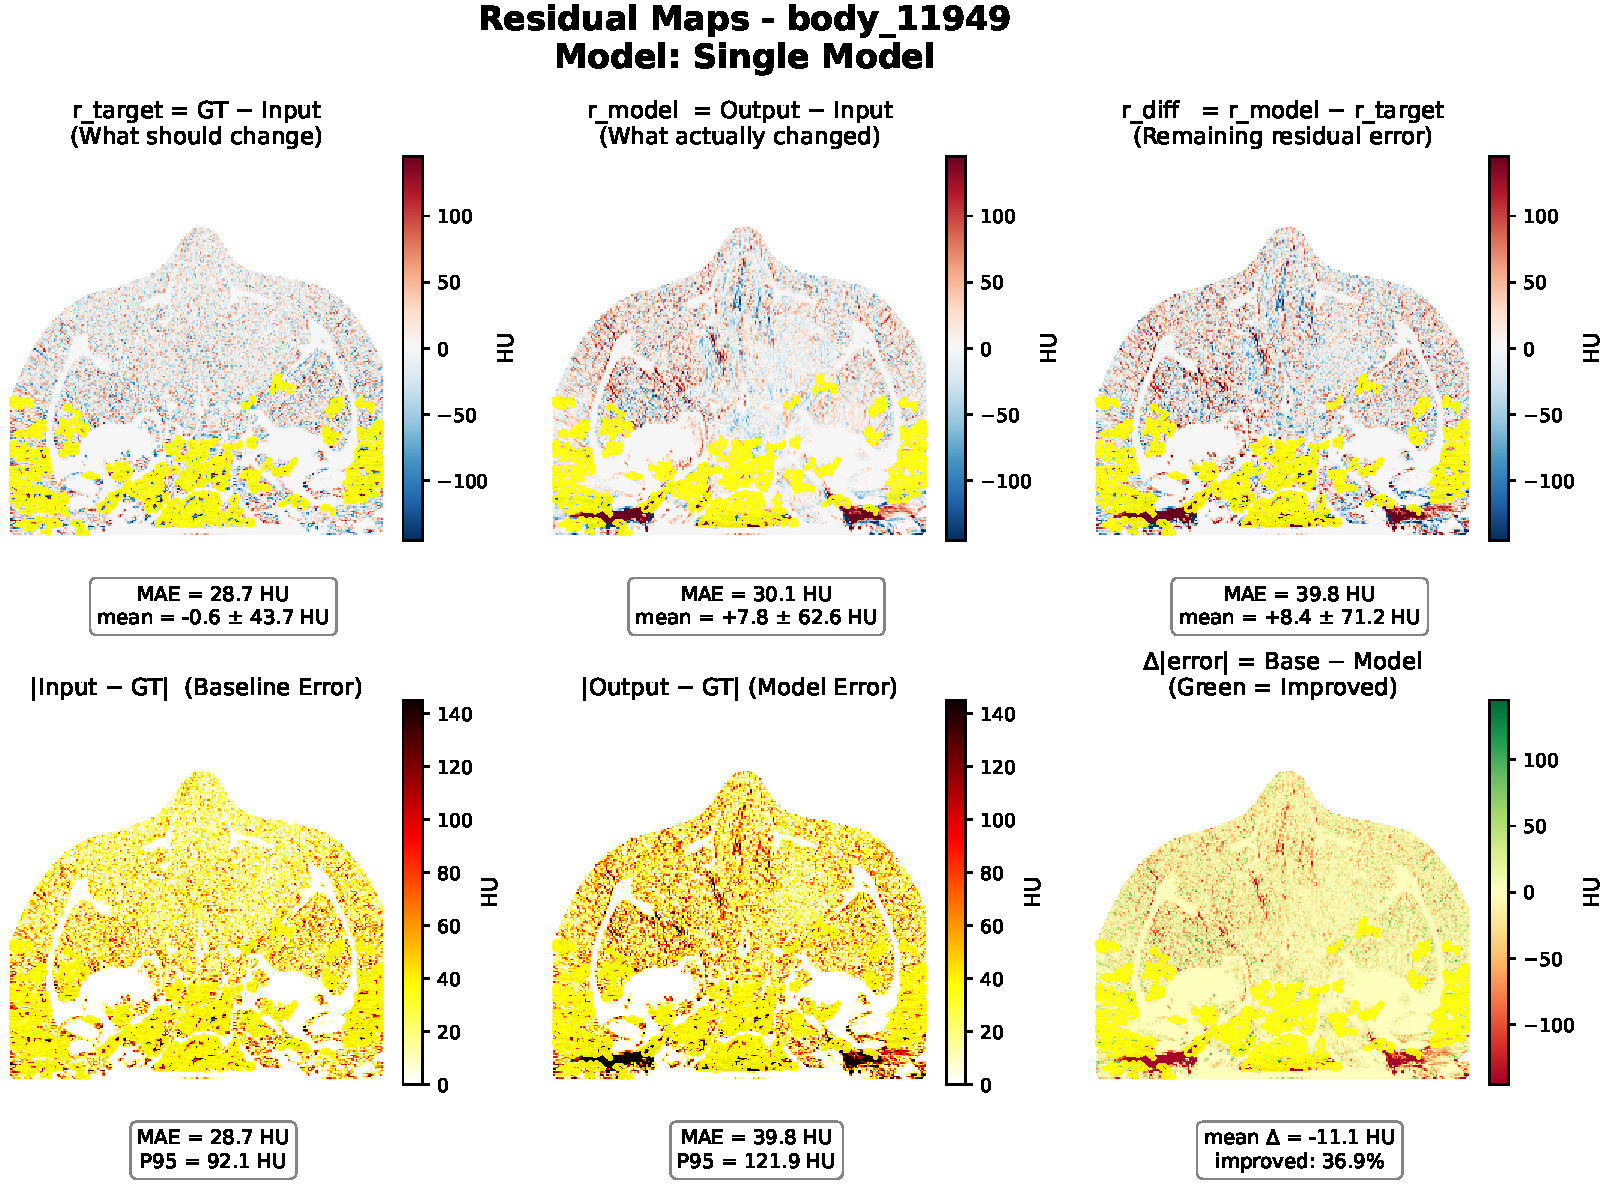
\includegraphics[width=\linewidth]{Figures/Generated/evaluation_final/Residuals/residual_least_structural_improvement_01_s0716.pdf}
\medskip
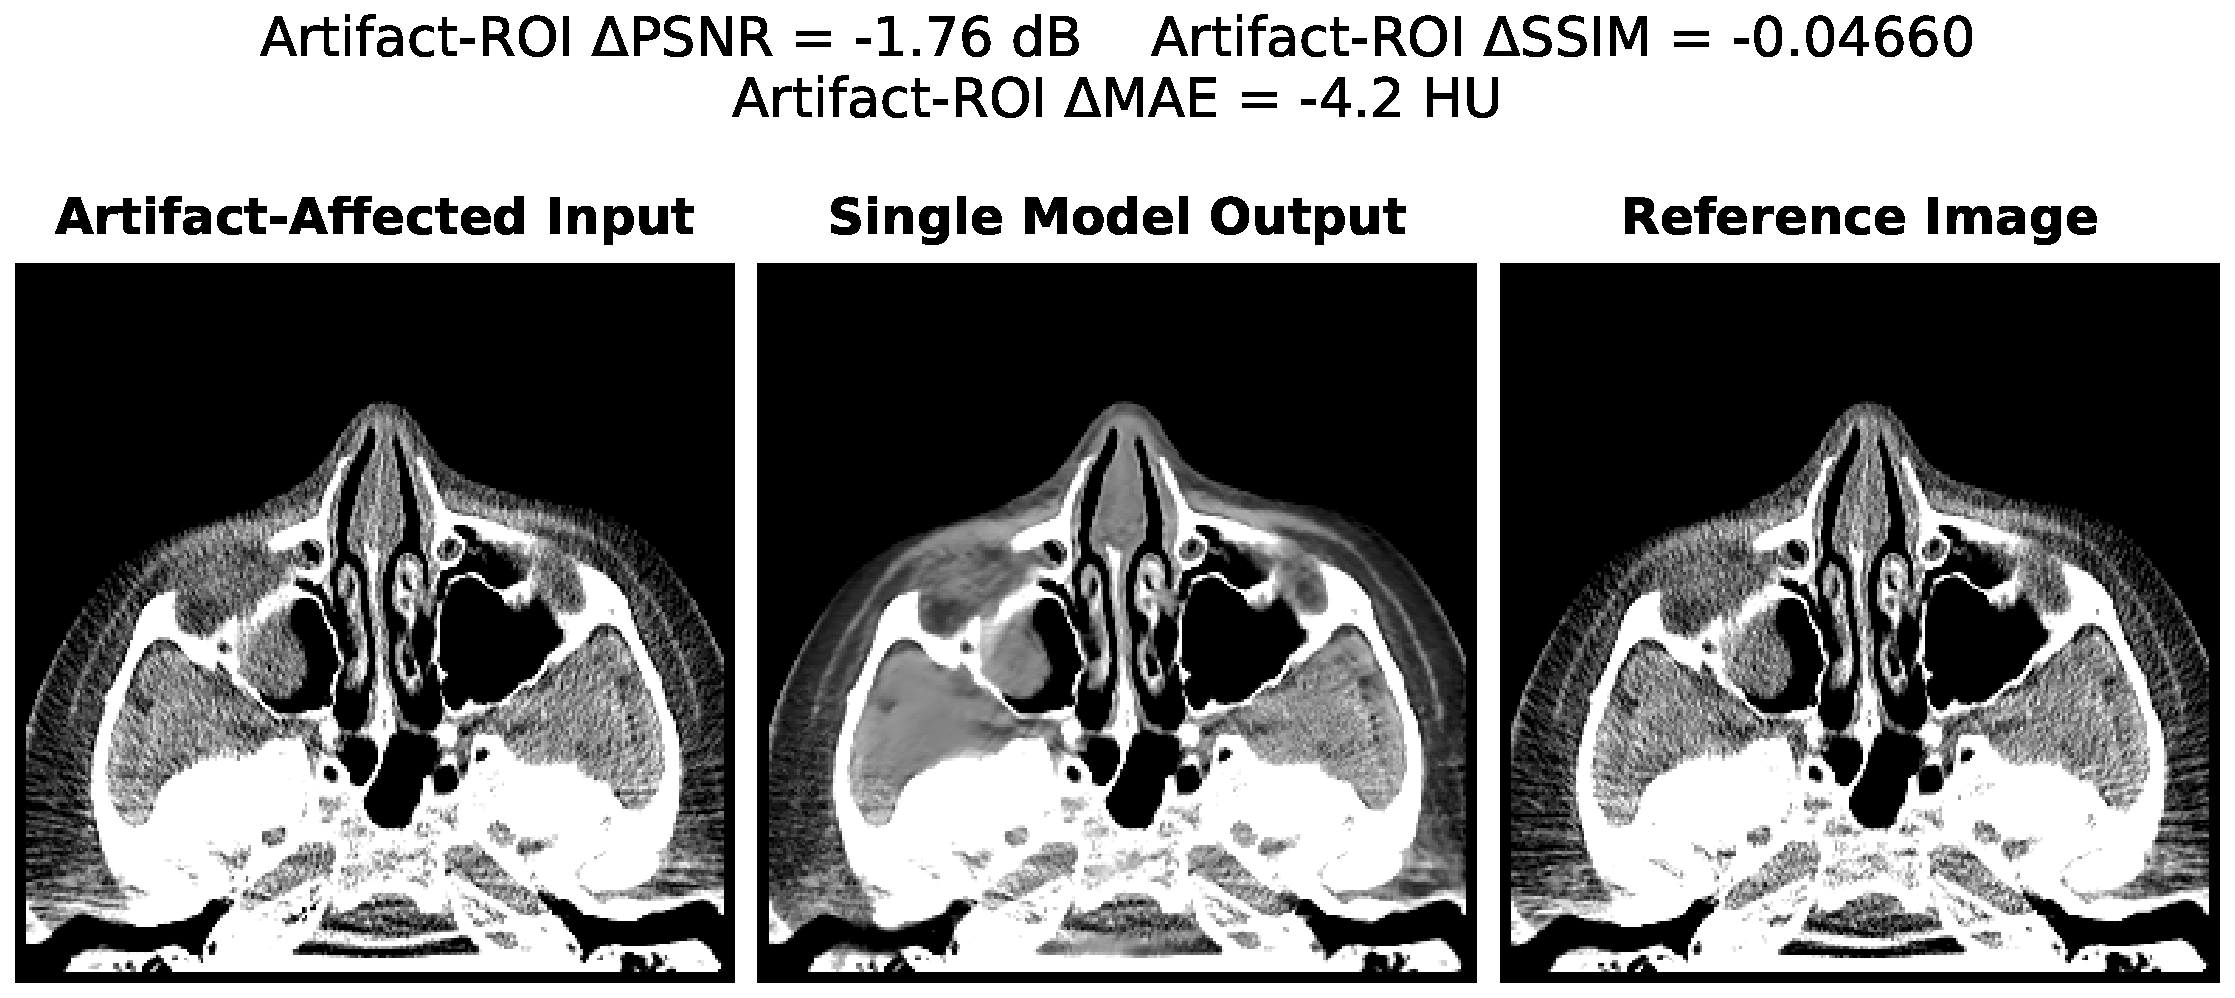
\includegraphics[width=0.94\linewidth]{Figures/Generated/evaluation_final/Residuals/visualization_least_structural_improvement_01_s0716.pdf}
\captionsetup{skip=2pt}
\caption[Least Artifact-ROI $\Delta$SSIM: body\_11949]{Residual map (top) and reconstruction visualization (bottom) for case body\_11949 (test-set index 0716), selected among the three lowest artifact-ROI $\Delta$SSIM values ($\Delta\mathrm{SSIM}_{\mathrm{ROI}}=-0.0466$; global $\Delta\mathrm{SSIM}=-0.0497$; $\Delta\mathrm{PSNR}=-4.31$~dB). The yellow contour delimits the artifact ROI; all error maps are restricted to the body mask.}
\label{fig:residual-least-structural-improvement-0716}
\end{figure}

\begin{figure}[!htbp]
\centering
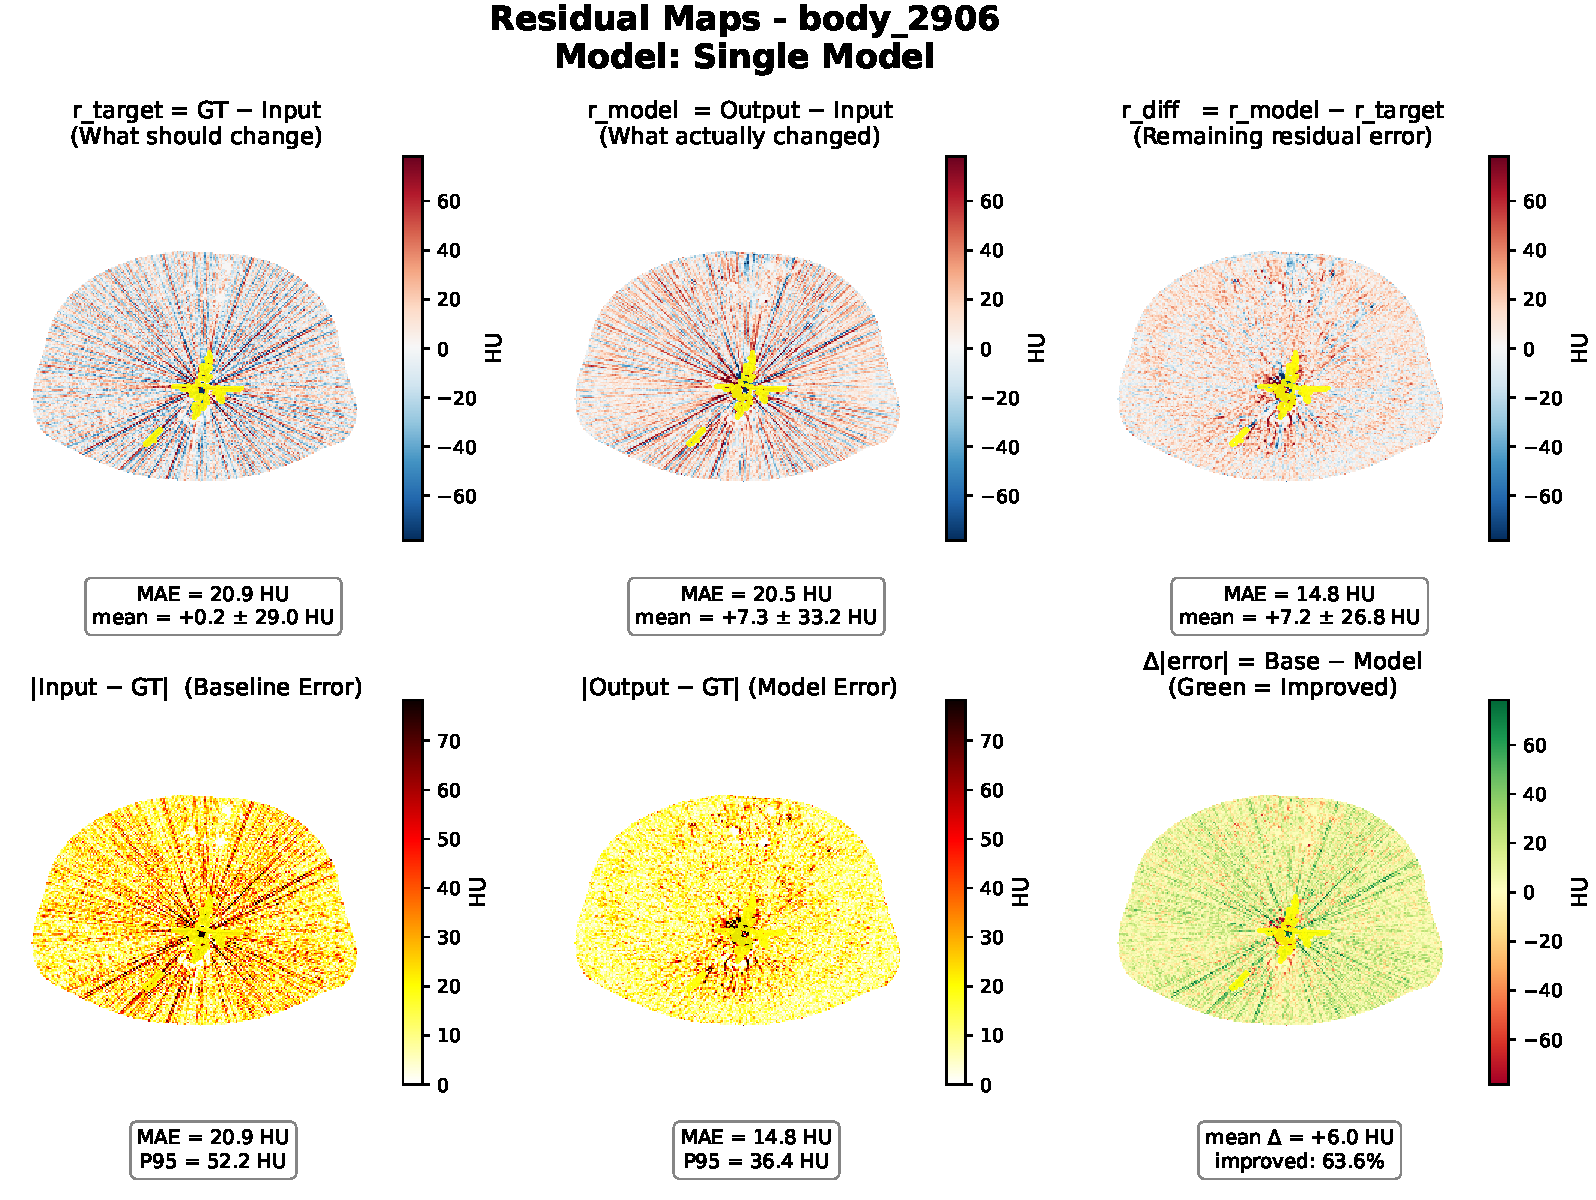
\includegraphics[width=\linewidth]{Figures/Generated/evaluation_final/Residuals/residual_least_structural_improvement_02_s1122.pdf}
\medskip
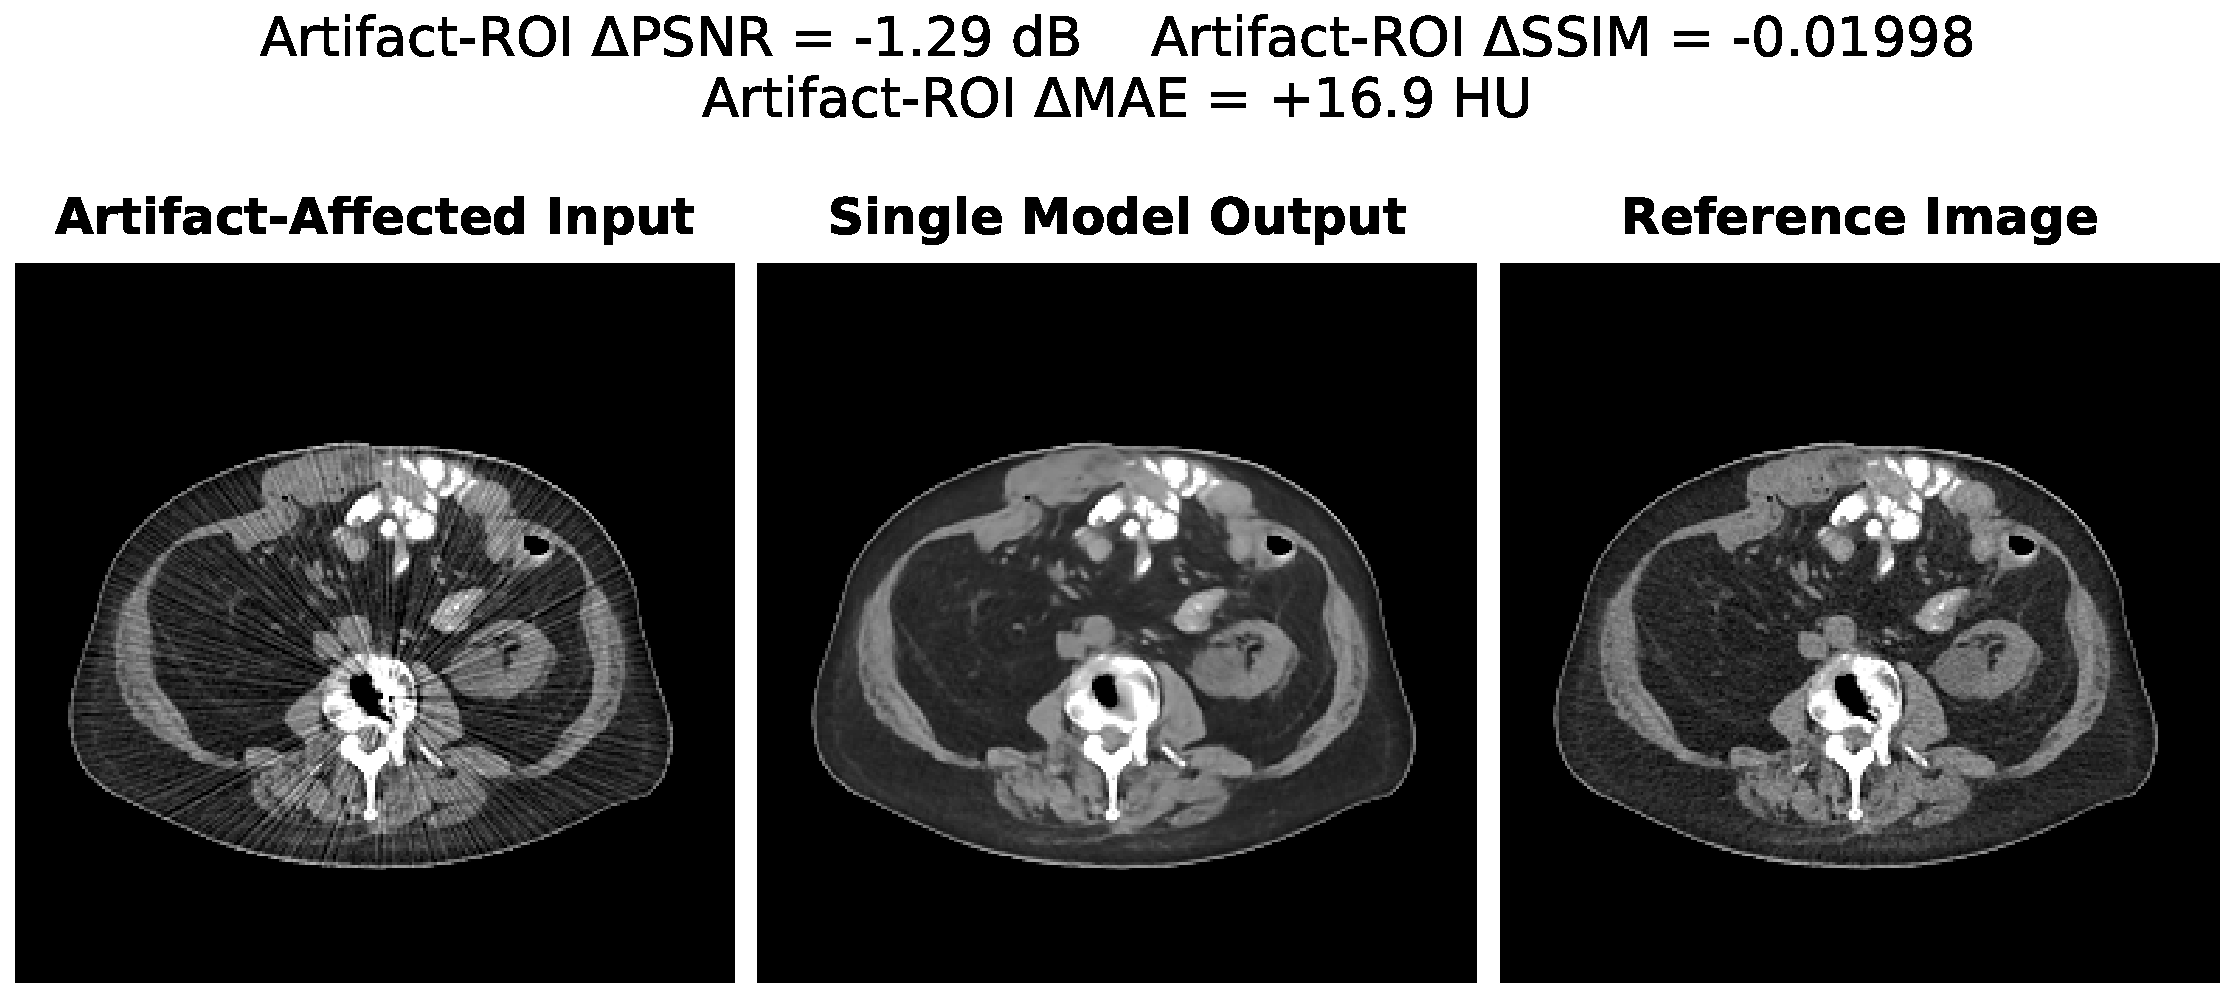
\includegraphics[width=0.94\linewidth]{Figures/Generated/evaluation_final/Residuals/visualization_least_structural_improvement_02_s1122.pdf}
\captionsetup{skip=2pt}
\caption[Least Artifact-ROI $\Delta$SSIM: body\_2906]{Residual map (top) and reconstruction visualization (bottom) for case body\_2906 (test-set index 1122), selected among the three lowest artifact-ROI $\Delta$SSIM values ($\Delta\mathrm{SSIM}_{\mathrm{ROI}}=-0.0200$; global $\Delta\mathrm{SSIM}=+0.0740$; $\Delta\mathrm{PSNR}=+0.38$~dB). The yellow contour delimits the artifact ROI; all error maps are restricted to the body mask.}
\label{fig:residual-least-structural-improvement-1122}
\end{figure}

\begin{figure}[!htbp]
\centering
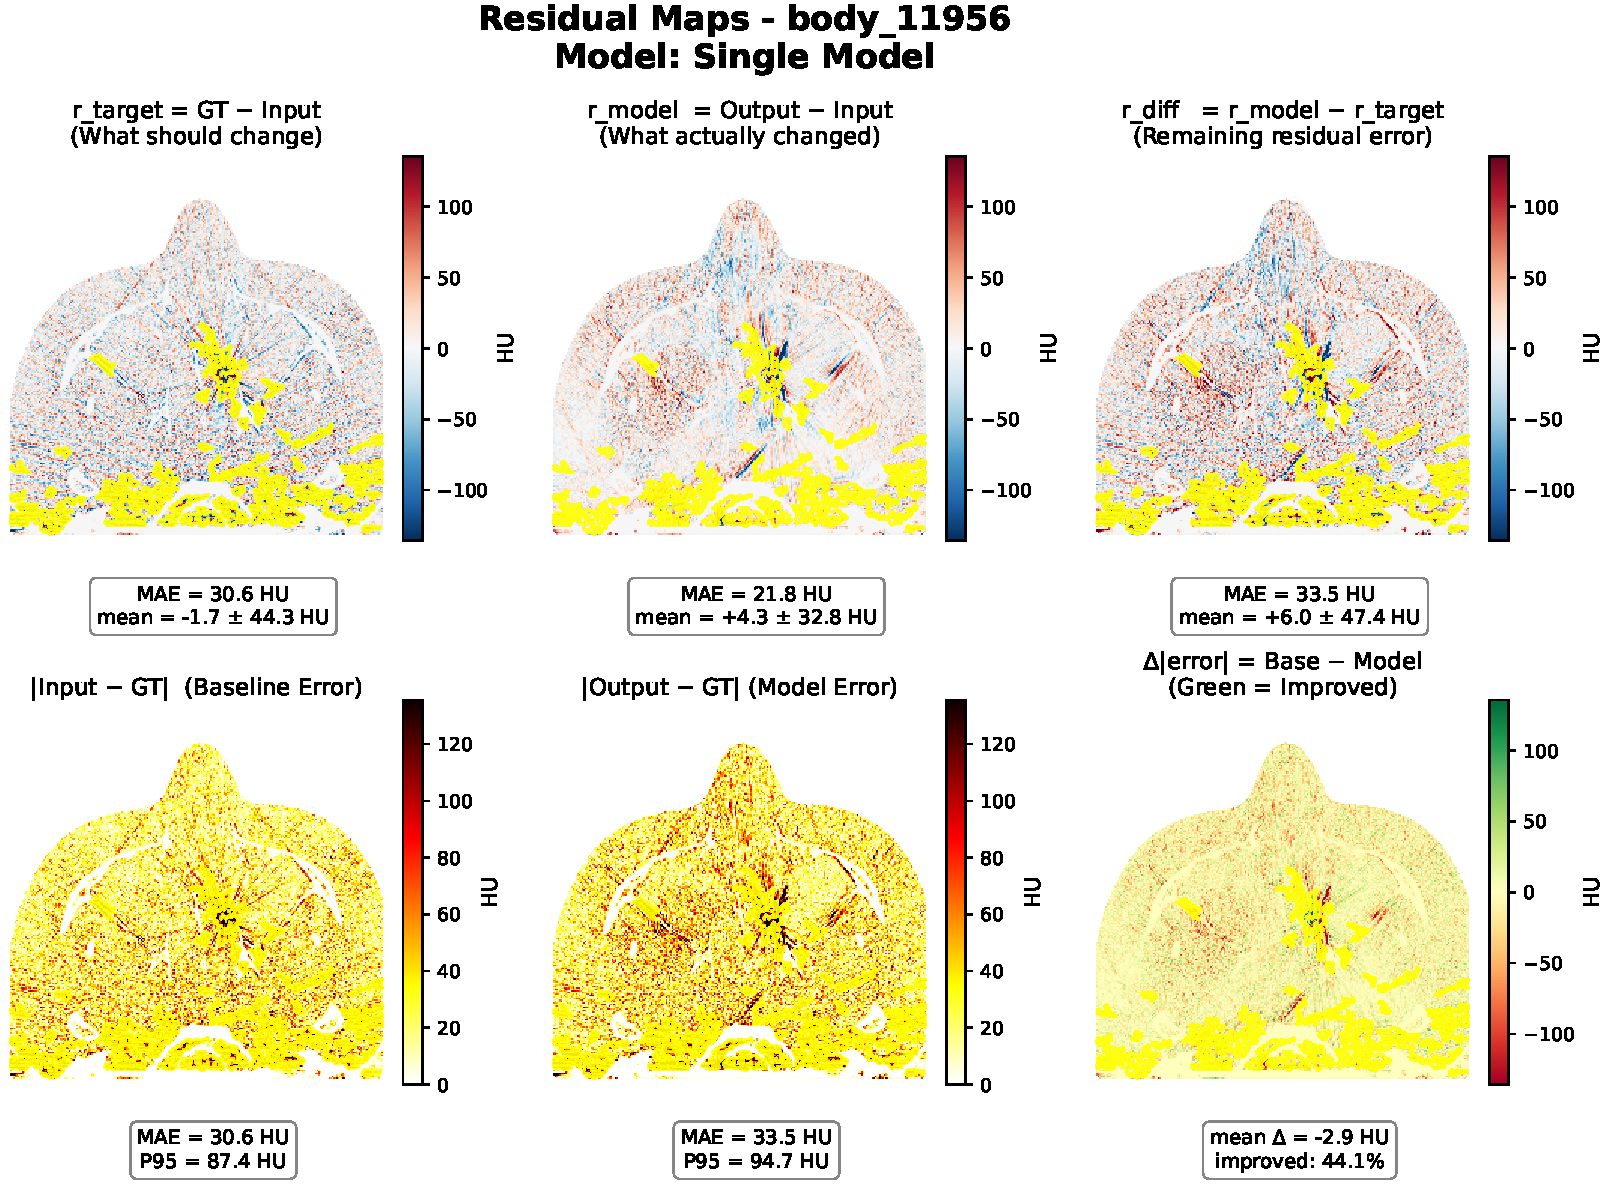
\includegraphics[width=\linewidth]{Figures/Generated/evaluation_final/Residuals/residual_least_structural_improvement_03_s0723.pdf}
\medskip
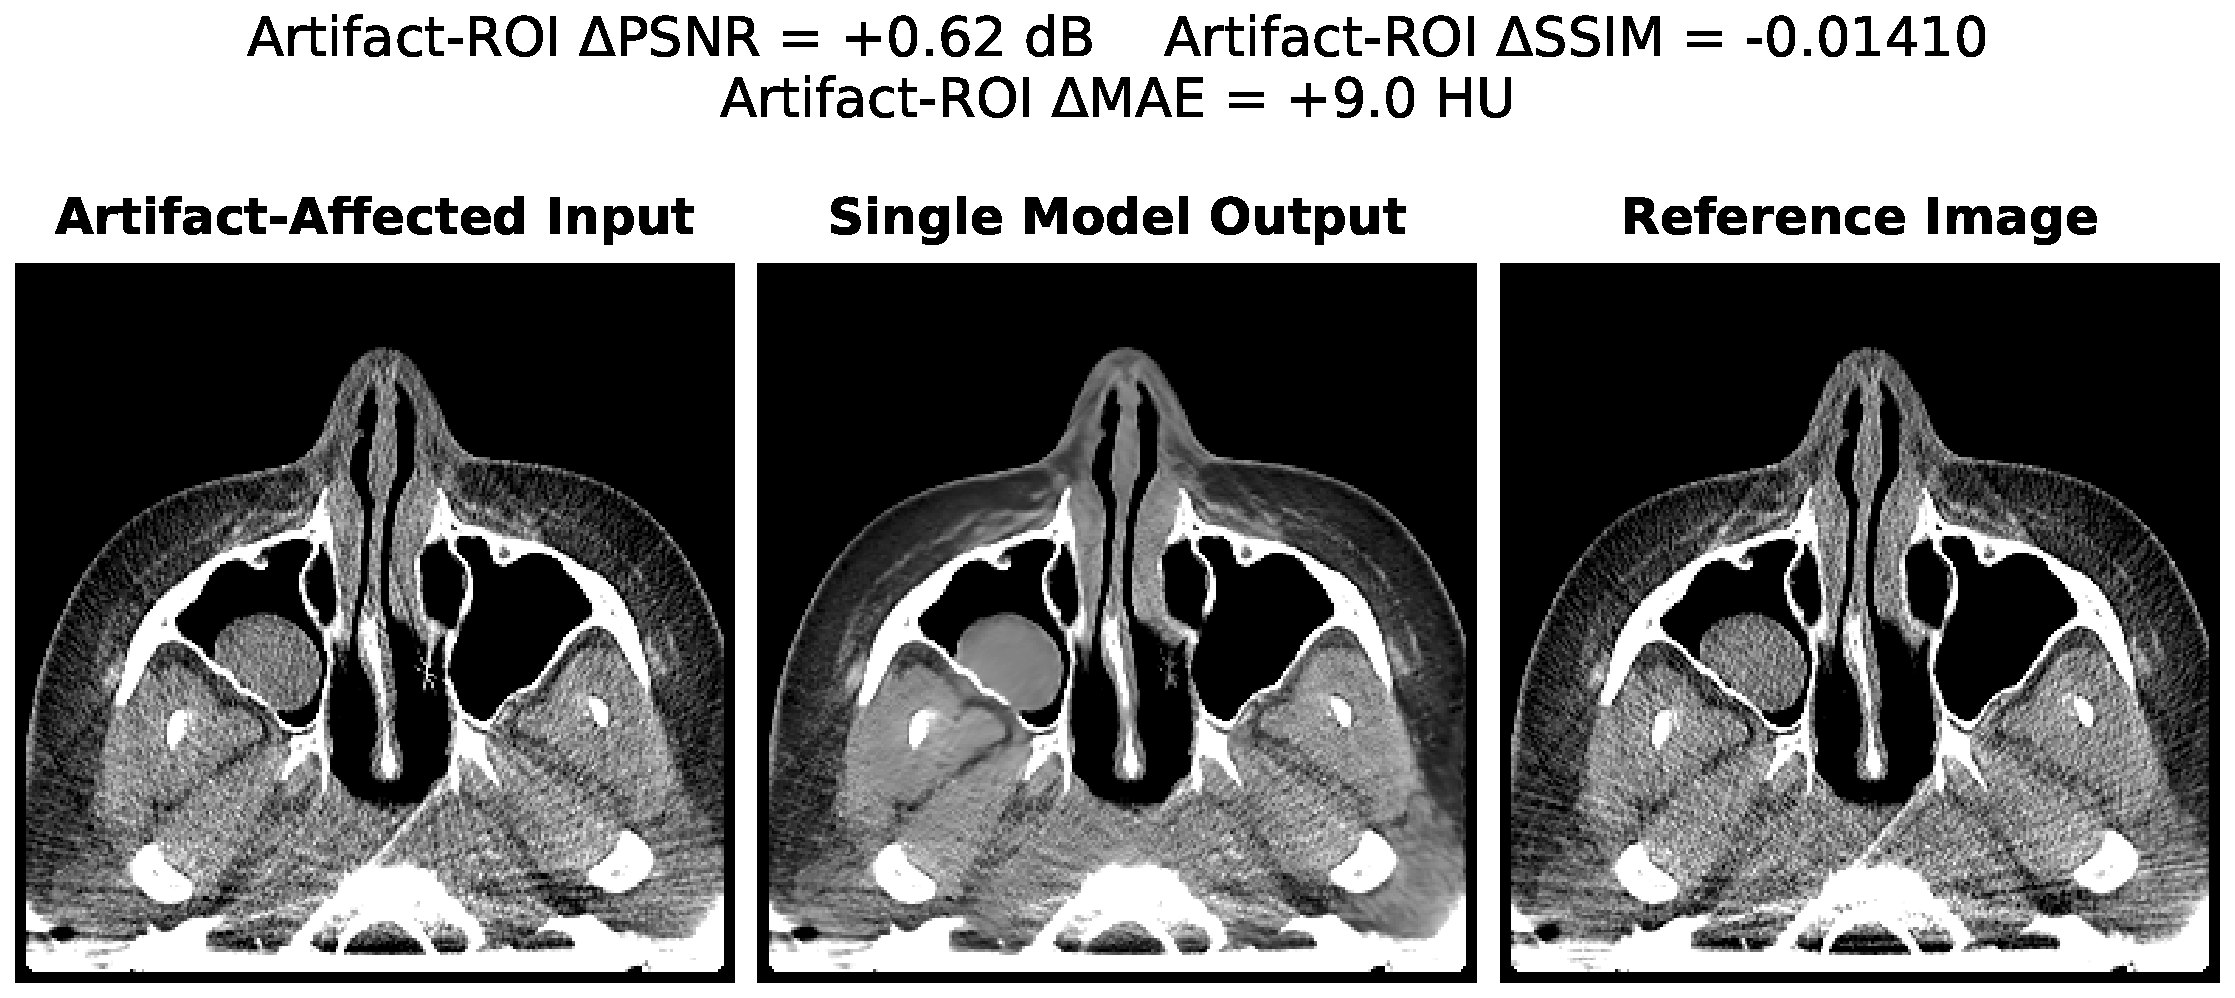
\includegraphics[width=0.94\linewidth]{Figures/Generated/evaluation_final/Residuals/visualization_least_structural_improvement_03_s0723.pdf}
\captionsetup{skip=2pt}
\caption[Least Artifact-ROI $\Delta$SSIM: body\_11956]{Residual map (top) and reconstruction visualization (bottom) for case body\_11956 (test-set index 0723), selected among the three lowest artifact-ROI $\Delta$SSIM values ($\Delta\mathrm{SSIM}_{\mathrm{ROI}}=-0.0141$; global $\Delta\mathrm{SSIM}=-0.0345$; $\Delta\mathrm{PSNR}=-0.64$~dB). The yellow contour delimits the artifact ROI; all error maps are restricted to the body mask.}
\label{fig:residual-least-structural-improvement-0723}
\end{figure}

\FloatBarrier

\section{Paired Comparison Single x Dual Model}
\label{sec:paired-comparison-single-dual}

\subsection{Statistical Analysis per\acrshort{roi}}
\label{sec:statistical-analysis-roi}

This section formally tests this study's main hypothesis, that structure improves in the Artifact Zone, and describes preservation in the Clean Zone as a complement. As before, per-slice metrics were always averaged per patient before any summary or test ($n=41$), and 95\% confidence intervals were obtained by resampling patients 10,000 times. In the Artifact Zone, the question is simply whether the model improved on the input, so the signed changes in\acrshort{psnr},\acrshort{ssim}, and\acrshort{mae} were analyzed. For each model, the sign test was applied to each of the three metrics, with a joint Holm correction across them.

\begin{table}[htbp]
\centering
\small
\begin{tabular}{lccc}
\multicolumn{4}{c}{\textbf{Artifact ROI: SSIM}} \\[3pt]
\toprule
\textbf{Model} & \textbf{Mean improvement} & \textbf{95\% BCa CI} & \textbf{$p$ (Holm)} \\
\midrule
Single Model & $0.3279$ & $[0.2963; 0.3548]$ & $2.73\times10^{-12}$ \\
Dual Model & $0.3266$ & $[0.2947; 0.3534]$ & $2.73\times10^{-12}$ \\
\bottomrule
\end{tabular}
\captionsetup{skip=2pt}
\caption[Artifact-ROI SSIM improvement]{SSIM improvement over the corrupted input in the Artifact ROI.\tablecaptionnote{Patient-level Artifact-ROI improvement ($n=41$). Two-sided exact binomial sign-test $p$-values, Holm-adjusted across PSNR, SSIM, and MAE separately for each model.}}
\label{tab:roi-artifact-improvement-ssim}
\end{table}

\begin{table}[htbp]
\centering
\small
\begin{tabular}{lccc}
\multicolumn{4}{c}{\textbf{Artifact ROI: PSNR}} \\[3pt]
\toprule
\textbf{Model} & \textbf{Mean improvement (dB)} & \textbf{95\% BCa CI} & \textbf{$p$ (Holm)} \\
\midrule
Single Model & $11.86$ & $[10.90; 12.59]$ & $2.73\times10^{-12}$ \\
Dual Model & $11.84$ & $[10.91; 12.55]$ & $2.73\times10^{-12}$ \\
\bottomrule
\end{tabular}
\captionsetup{skip=2pt}
\caption[Artifact-ROI PSNR improvement]{PSNR improvement over the corrupted input in the Artifact ROI.\tablecaptionnote{Patient-level Artifact-ROI improvement ($n=41$). Two-sided exact binomial sign-test $p$-values, Holm-adjusted across PSNR, SSIM, and MAE separately for each model.}}
\label{tab:roi-artifact-improvement-psnr}
\end{table}

\begin{table}[htbp]
\centering
\small
\begin{tabular}{lccc}
\multicolumn{4}{c}{\textbf{Artifact ROI: MAE}} \\[3pt]
\toprule
\textbf{Model} & \textbf{Mean reduction (HU)} & \textbf{95\% BCa CI} & \textbf{$p$ (Holm)} \\
\midrule
Single Model & $98.38$ & $[91.75; 104.24]$ & $2.73\times10^{-12}$ \\
Dual Model & $98.33$ & $[91.84; 104.06]$ & $2.73\times10^{-12}$ \\
\bottomrule
\end{tabular}
\captionsetup{skip=2pt}
\caption[Artifact-ROI MAE reduction]{MAE reduction over the corrupted input in the Artifact ROI.\tablecaptionnote{Patient-level Artifact-ROI improvement ($n=41$). Positive $\Delta$MAE denotes error reduction. Two-sided exact binomial sign-test $p$-values, Holm-adjusted across PSNR, SSIM, and MAE separately for each model.}}
\label{tab:roi-artifact-improvement-mae}
\end{table}
\FloatBarrier

\autoref{tab:roi-artifact-improvement-ssim}, \autoref{tab:roi-artifact-improvement-psnr}, and \autoref{tab:roi-artifact-improvement-mae} show improvement in all three metrics in the Artifact Zone for both models. These results support the primary hypothesis of structural improvement in the region directly affected by the artifact.

\begin{table}[htbp]
\centering
\small
\begin{tabular}{lccc}
\toprule
\textbf{Metric} & \textbf{$\Delta_{\mathrm{Dual}}-\Delta_{\mathrm{Single}}$} & \textbf{95\% BCa CI} & \textbf{$p$ (Holm)} \\
\midrule
$\Delta$SSIM & $-0.0013$ & $[-0.0025; 0.0002]$ & $0.0345$ \\
$\Delta$PSNR (dB) & $-0.019$ & $[-0.085; 0.060]$ & $0.533$ \\
$\Delta$MAE (HU) & $-0.049$ & $[-0.318; 0.345]$ & $0.422$ \\
\bottomrule
\end{tabular}
\captionsetup{skip=2pt}
\caption[Paired Artifact-ROI improvement comparison]{Patient-level paired comparison of improvement deltas in the Artifact ROI.\tablecaptionnote{Patient-level paired comparison of input-to-output improvement deltas ($n=41$). Differences are $\Delta_{\mathrm{Dual}}-\Delta_{\mathrm{Single}}$. Negative differences favor the Single Model for all metrics. The 95\% BCa bootstrap CIs use 10\,000 resamples. Two-sided exact binomial sign-test $p$-values are Holm-adjusted across the three Artifact-ROI metrics.}}
\label{tab:roi-artifact-paired-comparison}
\end{table}
\FloatBarrier


In the direct comparison of improvement deltas in the Artifact Zone (\autoref{tab:roi-artifact-paired-comparison}), the structural-similarity difference was small but remained statistically significant after adjustment, favoring the Single Model. The other two metrics did not show an adjusted between-architecture difference.

In the Clean Zone, the question is different: the goal is to see how well the tissue away from the artifact was left unchanged, since ideally there should be no change at all relative to the input. So the average per-slice $|\Delta|$ was calculated for each patient, where lower values mean the reconstruction stayed closer to the input. Because no specific ``close enough to zero'' limit was set in advance, it is not possible to formally test or conclude that the change is equivalent to zero. Thus, \autoref{tab:roi-distant-preservation-ssim}, \autoref{tab:roi-clean-preservation-psnr}, \autoref{tab:roi-clean-preservation-mae} report the size of the change and its confidence intervals, without a $p$-value against zero.

\begin{table}[htbp]
\centering
\small
\begin{tabular}{lcc}
\multicolumn{3}{c}{\textbf{Clean ROI: SSIM}} \\[3pt]
\toprule
\textbf{Model} & \textbf{Mean $|\Delta|$} & \textbf{95\% BCa CI} \\
\midrule
Single Model & $0.0599$ & $[0.0503; 0.0754]$ \\
Dual Model & $0.0595$ & $[0.0499; 0.0748]$ \\
\bottomrule
\end{tabular}
\captionsetup{skip=2pt}
\captionof{table}[Clean-ROI SSIM preservation magnitude]{Magnitude of SSIM input-to-output change in the Clean ROI.\tablecaptionnote{Patient-level mean absolute per-slice input-to-output change ($n=41$). Lower values are closer to zero. No equivalence margin or hypothesis test against zero was prespecified.}}
\label{tab:roi-distant-preservation-ssim}
\end{table}

\begin{table}[htbp]
\centering
\small
\begin{tabular}{lcc}
\multicolumn{3}{c}{\textbf{Clean ROI: PSNR}} \\[3pt]
\toprule
\textbf{Model} & \textbf{Mean $|\Delta|$ (dB)} & \textbf{95\% BCa CI} \\
\midrule
Single Model & $1.99$ & $[1.66; 2.34]$ \\
Dual Model & $1.97$ & $[1.64; 2.33]$ \\
\bottomrule
\end{tabular}
\captionsetup{skip=2pt}
\caption[Clean-ROI PSNR preservation magnitude]{Magnitude of PSNR input-to-output change in the Clean ROI.\tablecaptionnote{Patient-level mean absolute per-slice input-to-output change ($n=41$). Lower values are closer to zero. No equivalence margin or hypothesis test against zero was prespecified.}}
\label{tab:roi-clean-preservation-psnr}
\end{table}

\begin{table}[htbp]
\centering
\small
\begin{tabular}{lcc}
\multicolumn{3}{c}{\textbf{Clean ROI: MAE}} \\[3pt]
\toprule
\textbf{Model} & \textbf{Mean $|\Delta|$ (HU)} & \textbf{95\% BCa CI} \\
\midrule
Single Model & $4.30$ & $[3.60; 5.16]$ \\
Dual Model & $4.24$ & $[3.54; 5.08]$ \\
\bottomrule
\end{tabular}
\captionsetup{skip=2pt}
\caption[Clean-ROI MAE preservation magnitude]{Magnitude of MAE input-to-output change in the Clean ROI.\tablecaptionnote{Patient-level mean absolute per-slice input-to-output change ($n=41$). Lower values are closer to zero. No equivalence margin or hypothesis test against zero was prespecified.}}
\label{tab:roi-clean-preservation-mae}
\end{table}
\FloatBarrier
To compare the architectures on preservation in the Clean Zone, the Dual Model's advantage was defined for each patient as $|\Delta|_{\mathrm{Single}}-|\Delta|_{\mathrm{Dual}}$, and the sign test was applied, with a joint Holm correction across the three metrics. This is a separate comparison from the Artifact-Zone improvement above: here, what matters is the size of the change, and the better value is the one closest to zero. Positive values indicate a smaller change introduced by the Dual Model. This test answers only which model introduced a smaller change, not whether that change is clinically negligible.

\begin{table}[htbp]
\centering
\small
\begin{tabular}{lccc}
\toprule
\textbf{Metric} & \textbf{Dual preservation advantage} & \textbf{95\% BCa CI} & \textbf{$p$ (Holm)} \\
\midrule
SSIM & $0.000390$ & $[0.000056; 0.000642]$ & $3.37\times10^{-4}$ \\
PSNR (dB) & $0.020$ & $[-0.104; 0.069]$ & $0.0275$ \\
MAE (HU) & $0.066$ & $[-0.050; 0.155]$ & $0.00865$ \\
\bottomrule
\end{tabular}
\captionsetup{skip=2pt}
\caption[Paired Clean-ROI preservation advantage]{Relative preservation advantage of the Dual Model in the Clean ROI.\tablecaptionnote{Patient-level paired preservation advantage ($n=41$), defined as $|\Delta|_{\mathrm{Single}}-|\Delta|_{\mathrm{Dual}}$. Positive values favor the Dual Model because its mean absolute input-to-output change is smaller. The 95\% BCa bootstrap CIs use 10\,000 resamples, two-sided exact binomial sign-test $p$-values are Holm-adjusted across the three Clean-ROI metrics.}}
\label{tab:roi-clean-paired-preservation}
\end{table}

In the relative comparison (\autoref{tab:roi-clean-paired-preservation}), the Dual Model showed a smaller absolute change in\acrshort{psnr},\acrshort{ssim}, and\acrshort{mae} after the Holm correction. This suggests the Dual Model preserved the clean tissue somewhat better than the Single Model, but it does not prove the change was equivalent to none at all.

The computational performance (inference latency and throughput) of the model selected for external evaluation is characterized in \autoref{sec:appendix-computational-performance}.

\subsection{Global Statistical Analysis}
As in the\acrshort{roi} analysis, global per-slice metrics were averaged per patient before any summary or statistical test, giving $n=41$ independent patients. So the means, 95\% confidence intervals, and $p$-values in this section's tables all refer to per-patient averages, with each patient counted equally.

The tables in this section analyze the global metrics, calculated over all pixels of the body mask of each slice (background excluded), as a complementary confirmation of the main hypothesis of structural improvement.

Checking the distribution of the per-patient values for $\Delta$SSIM and $\Delta$MAE showed that they were skewed, not evenly spread around the middle. Because of this, the main evidence for these two metrics came from the sign test, which simply asks how often the model did better than the input, without assuming the improvements are symmetrically distributed. For $\Delta$PSNR, whose per-patient values showed no such skew, the two-sided one-sample $t$-test was used instead, to test the average improvement directly.

This distribution check was performed separately for each model and supported the same inference rule for both architectures: sign tests for structural similarity and absolute error, and a one-sample $t$-test for peak signal-to-noise ratio. The diagnostic values are retained in the analysis records rather than repeated in the narrative.

\begin{table}[htbp]
\centering
\small
\begin{tabular}{lccc}
\multicolumn{4}{c}{\textbf{Reconstruction Quality: SSIM}} \\[3pt]
\toprule
\textbf{Model} & \textbf{Mean improvement} & \textbf{95\% BCa CI} & \textbf{$p$ (Holm)} \\
\midrule
Single Model & $0.0891$ & $[0.0744; 0.1075]$ & $7.64\times10^{-11}$ \\\\
Dual Model & $0.0879$ & $[0.0731; 0.1062]$ & $7.64\times10^{-11}$ \\\\
\bottomrule
\end{tabular}
\captionsetup{skip=2pt}
\caption[SSIM improvement over corrupted input]{Global SSIM improvement over the corrupted input on the test set.\tablecaptionnote{Global body-mask-aware metric, aggregated at the patient level ($n=41$). No ROI restriction. Two-sided exact binomial sign-test $p$-values, Holm-adjusted separately within each model across SSIM, PSNR, and MAE.}}
\label{tab:ablation_improvement_ssim}
\end{table}
\begin{table}[htbp]
\centering
\small
\begin{tabular}{lccc}
\multicolumn{4}{c}{\textbf{Reconstruction Quality: PSNR}} \\[3pt]
\toprule
\textbf{Model} & \textbf{Mean improvement (dB)} & \textbf{95\% $t$ CI} & \textbf{$p$ (Holm)} \\
\midrule
Single Model & $7.11$ & $[6.35; 7.87]$ & $4.53\times10^{-21}$ \\\\
Dual Model & $7.06$ & $[6.30; 7.81]$ & $4.42\times10^{-21}$ \\\\
\bottomrule
\end{tabular}
\captionsetup{skip=2pt}
\caption[PSNR improvement over corrupted input]{Global PSNR improvement over the corrupted input on the test set.\tablecaptionnote{Global body-mask-aware metric, aggregated at the patient level ($n=41$). No ROI restriction. Two-sided one-sample $t$-test $p$-values, Holm-adjusted separately within each model across SSIM, PSNR, and MAE.}}
\label{tab:ablation_improvement_psnr}
\end{table}
\begin{table}[htbp]
\centering
\small
\begin{tabular}{lccc}
\multicolumn{4}{c}{\textbf{Reconstruction Quality: MAE}} \\[3pt]
\toprule
\textbf{Model} & \textbf{Mean reduction (HU)} & \textbf{95\% BCa CI} & \textbf{$p$ (Holm)} \\
\midrule
Single Model & $15.72$ & $[12.94; 20.14]$ & $7.64\times10^{-11}$ \\\\
Dual Model & $15.54$ & $[12.79; 19.88]$ & $7.64\times10^{-11}$ \\\\
\bottomrule
\end{tabular}
\captionsetup{skip=2pt}
\caption[MAE reduction over corrupted input]{Global MAE reduction over the corrupted input on the test set.\tablecaptionnote{Global body-mask-aware metric, aggregated at the patient level ($n=41$). No ROI restriction. Positive $\Delta$MAE denotes error reduction. Two-sided exact binomial sign-test $p$-values, Holm-adjusted separately within each model across SSIM, PSNR, and MAE.}}
\label{tab:ablation_improvement_mae}
\end{table}
\FloatBarrier

\autoref{tab:ablation_improvement_ssim}, \autoref{tab:ablation_improvement_psnr}, and \autoref{tab:ablation_improvement_mae} show that both architectures improved global reconstruction quality relative to the corrupted input. All patient-level tests remained significant after the prespecified Holm adjustment. The tables retain the effect estimates, confidence intervals, and test results; their numerical scales should not be compared directly because the metrics answer different questions.

These tests confirm that each architecture improves upon the corrupted input, but they do not constitute a direct comparison between architectures. This distinction is essential: small $p$-values in \autoref{tab:ablation_improvement_ssim}, \autoref{tab:ablation_improvement_psnr}, \autoref{tab:ablation_improvement_mae} do not, by themselves, allow one to claim that one architecture is superior to the other.

The direct comparison between architectures is presented in \autoref{tab:workflow-paired-comparison}. For each patient, the difference in improvement between the two models was tested with a jointly adjusted sign test. The confidence intervals describe the magnitude of the average difference, whereas the test results describe how consistently one architecture prevailed. Negative values favor the Single Model.

\begin{table}[htbp]
\centering
\small
\begin{tabular}{cccc}
\multicolumn{4}{c}{\textbf{Dual Model $-$ Single Model: Improvement Deltas}} \\[3pt]
\hline
\textbf{Metric} & \textbf{Mean Difference} & \textbf{95\% BCa CI} & \textbf{$p$ (sign test; Holm)} \\
\hline
$\Delta$SSIM & $-0.0012$ & $[-0.0015; -0.0010]$ & $2.35\times10^{-9}$ \\
$\Delta$PSNR (dB) & $-0.054$ & $[-0.107; -0.017]$ & $2.75\times10^{-2}$ \\
$\Delta$MAE (HU) & $-0.186$ & $[-0.338; -0.091]$ & $8.62\times10^{-4}$ \\
\hline
\end{tabular}
\captionsetup{skip=2pt}
\caption[Paired Single vs Dual Model comparison]{Patient-level paired comparison of improvement deltas between architectures ($n=41$).\tablecaptionnote{Differences of patient-level input-to-output improvement deltas (Dual Model $-$ Single Model), with 95\% BCa bootstrap CIs (10\,000 resamples). Two-sided exact binomial sign-test $p$-values are Holm-adjusted across PSNR, SSIM, and MAE. Negative differences favor the Single Model for all three metrics.}}
\label{tab:workflow-paired-comparison}
\end{table}
\FloatBarrier

The paired estimates favor the Single Model globally, but the absolute differences are small. They indicate a modest numerical advantage rather than evidence that either architecture is clinically superior. The bar chart summarizes the similar global improvement obtained by both models.

\begin{figure}[htbp]
\centering
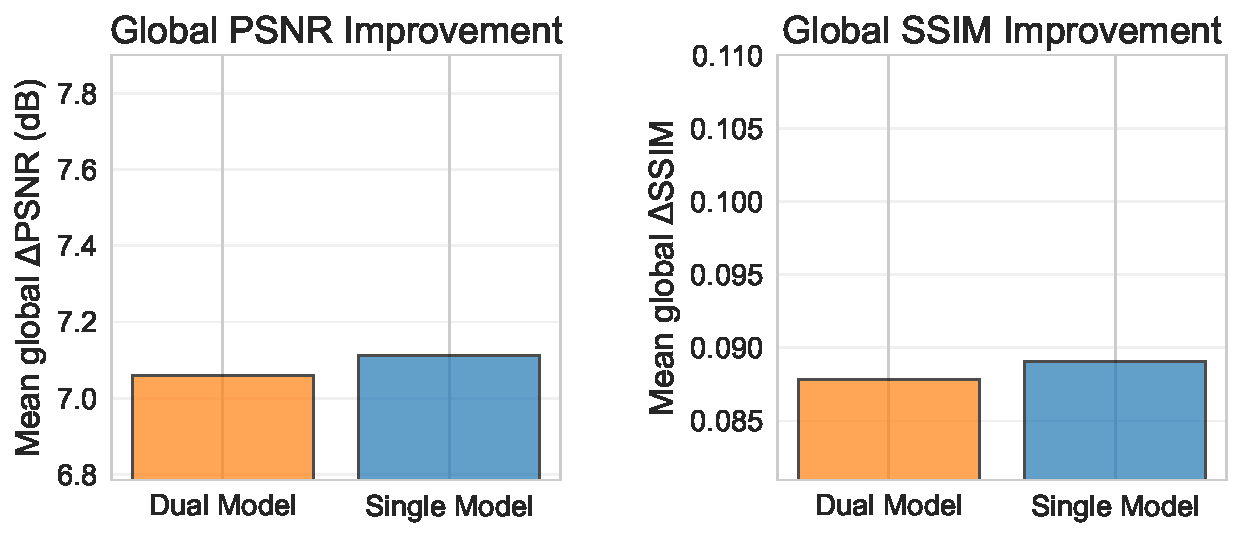
\includegraphics[width=0.95\linewidth]{Figures/Generated/paired/comparison-bar-charts-76dfb4b9.pdf}
\captionsetup{skip=2pt}
\graphiccaption[Global PSNR and SSIM improvement]{Global PSNR and SSIM improvement over the corrupted input for the Single and Dual Models on the test set.}
\end{figure}

\FloatBarrier

\section{External and Physician's Evaluation }
\label{sec:external-evatluation-doctors}

\subsection{Capture Status and Participants}
% To fill: final number of recruited readers, completed responses, and actual data-collection closing dates.

The external evaluation consists of a paired comparison blinded to the processing label: in each case, readers simultaneously view the artifact input and the model output, identified only as ``Image A'' and ``Image B''. The left/right position is counterbalanced across readers and kept constant between a case and its hidden repeat. Each session presents 19 comparisons: 2 training cases (excluded from the analysis), 15 main cases, and 2 hidden repeats of previously presented cases, used exclusively to assess intra-reader consistency. Physicians were recruited directly by the researcher, with self-declaration of clinical\acrshort{ct} use with a minimum monthly frequency. No name, contact information, professional registration number, or proof of qualification was collected.

\autoref{tab:external-reader-recruitment} summarizes the status of recruitment and response completion.

\begin{table}[htbp]
\centering
\small
\begin{tabular}{lc}
\toprule
\textbf{Indicator} & \textbf{Value} \\
\midrule
Total Readers & 5 \\
Total valid responses (readers $\times$ 15 main cases) & 75 \\
Data collection start date & 27-08-2026 \\
Data collection closing date & 10-09-2026 \\
\bottomrule
\end{tabular}
\captionsetup{skip=2pt}
\caption[Recruitment and completion status]{Status of recruitment and response completion for the external evaluation.}
\label{tab:external-reader-recruitment}
\end{table}
\FloatBarrier

The self-reported characteristics of the readers who completed the evaluation are presented in \autoref{tab:external-reader-profile}. None of these variables allow individual identification of a participant.

\begin{table}[htbp]
\centering
\small
\begin{tabular}{llcc}
\toprule
\textbf{Variable} & \textbf{Category} & \textbf{N} & \textbf{\%} \\
\midrule
\multirow{2}{*}{Jurisdiction} & Brazil & 5 & 100 \\
\midrule
\multirow{3}{*}{CT usage frequency} & Monthly & 4 & 80 \\
                                          & Daily & 1 & 20 \\
\midrule
\multirow{4}{*}{CT experience (years)} & $<2$ & 2 & 40 \\
                                            & 2--5 & 1 & 20 \\
                                            & 6--10 & 1 & 20 \\
                                            & $>10$ & 1 & 20 \\
\midrule
\multirow{3}{*}{Experience with artifact reduction} & None & 4 & 80 \\
                                                         & Occasional & 1 & 20 \\
\midrule
\multirow{3}{*}{Monitor type} & Conventional & 3 & 60 \\
                                  & Unknown & 2 & 40 \\
\bottomrule
\end{tabular}
\captionsetup{skip=2pt}
\caption[Reader profile characteristics]{Self-reported characteristics of the readers who completed the external evaluation.}
\label{tab:external-reader-profile}
\end{table}
\FloatBarrier
The distribution by medical specialty is presented separately in \autoref{tab:external-reader-specialty}, given the larger number of categories.

\begin{table}[htbp]
\centering
\small
\begin{tabular}{lcc}
\toprule
\textbf{Specialty} & \textbf{N} & \textbf{\%} \\
\midrule
Radiology and Diagnostic Imaging & 1 & 20 \\
Internal Medicine or General Medicine & 1 & 20 \\
Orthopedics or Traumatology & 1 & 20 \\
Infectious Diseases & 1 & 20 \\
Other medical specialty & 1 & 20 \\
\bottomrule
\end{tabular}
\captionsetup{skip=2pt}
\caption[Reader specialty distribution]{Distribution by medical specialty of the readers who completed the external evaluation.}
\label{tab:external-reader-specialty}
\end{table}
\FloatBarrier

\subsection{Quantitative Characterization of Input--Output}
Before the professional evaluation, the global change produced by the \textit{Single Model} was characterized in the 15 main cases of the external set. The two training cases were excluded from this summary. Since these real exams do not have a clean reference, the metrics in \autoref{tab:external-input-output-global} compare exclusively the input image with the model output, within the body mask.

\begin{table}[htbp]
\centering
\small
\begin{tabular}{ccc}
\multicolumn{3}{c}{\textbf{Input--Output Similarity and Change}} \\[3pt]
\hline
\textbf{Metric} & \textbf{Mean $\pm$ SD} & \textbf{95\% CI} \\
\hline
SSIM (Input, Output) & $0.8953 \pm 0.0729$ & $[0.8572; 0.9290]$ \\
PSNR (Input, Output) (dB) & $33.14 \pm 6.49$ & $[29.95; 36.21]$ \\
MAE (Input, Output) (HU) & $21.12 \pm 15.26$ & $[14.54; 29.26]$ \\
\hline
\end{tabular}
\par\smallskip\footnotesize No artifact-free reference is available. Metrics were calculated within the manually corrected effective body mask and quantify input--output similarity or change; they do not measure artifact-removal accuracy or improvement.
\captionsetup{skip=2pt}
\caption[External input-output global metrics]{Global input--output metrics in the frozen external main set ($n=15$) for \texttt{singlehead-033-0.9511-ssim\_hu.keras}. Values are mean $\pm$ standard deviation; 95\% CIs are percentile bootstrap intervals for the mean.}
\label{tab:external-input-output-global}
\end{table}


The table shows heterogeneous input--output changes across the external cases. These results describe the preservation and overall modification of the external images, but cannot establish artifact-removal accuracy or clinical benefit without a clean reference.

To make this heterogeneity visible, the three cases with the highest and the three with the lowest input--output\acrshort{ssim} were selected descriptively. The former represent the pairs with the smallest overall structural change, while the latter represent those with the greatest change.

\begin{table}[htbp]
\centering
\small
\begin{tabular}{lcccc}
\multicolumn{5}{c}{\textbf{Illustrative External Cases Selected by Input--Output SSIM}} \\[3pt]
\hline
\textbf{Group} & \textbf{Case} & \textbf{SSIM} & \textbf{PSNR (dB)} & \textbf{MAE (HU)} \\
\hline
Least changed & Case 003 & $0.9809$ & $41.19$ & $8.76$ \\
 & Case 002 & $0.9756$ & $42.35$ & $8.10$ \\
 & Case 012 & $0.9586$ & $37.91$ & $9.64$ \\
Most changed & Case 015 & $0.7278$ & $23.32$ & $43.10$ \\
 & Case 005 & $0.7770$ & $20.77$ & $63.90$ \\
 & Case 008 & $0.8334$ & $33.53$ & $20.39$ \\
\hline
\end{tabular}
\par\smallskip\footnotesize Cases were selected only by the extremes of SSIM(Input, Output). High SSIM denotes less structural change between input and output; this ranking does not define artifact-removal quality or clinical acceptability.
\captionsetup{skip=2pt}
\caption[Illustrative external cases by input-output SSIM]{Descriptive external cases with the highest and lowest input--output SSIM values.}
\label{tab:external-ssim-extremes}
\end{table}

\begingroup
\setlength{\intextsep}{4pt}
\begin{figure}[H]
\centering
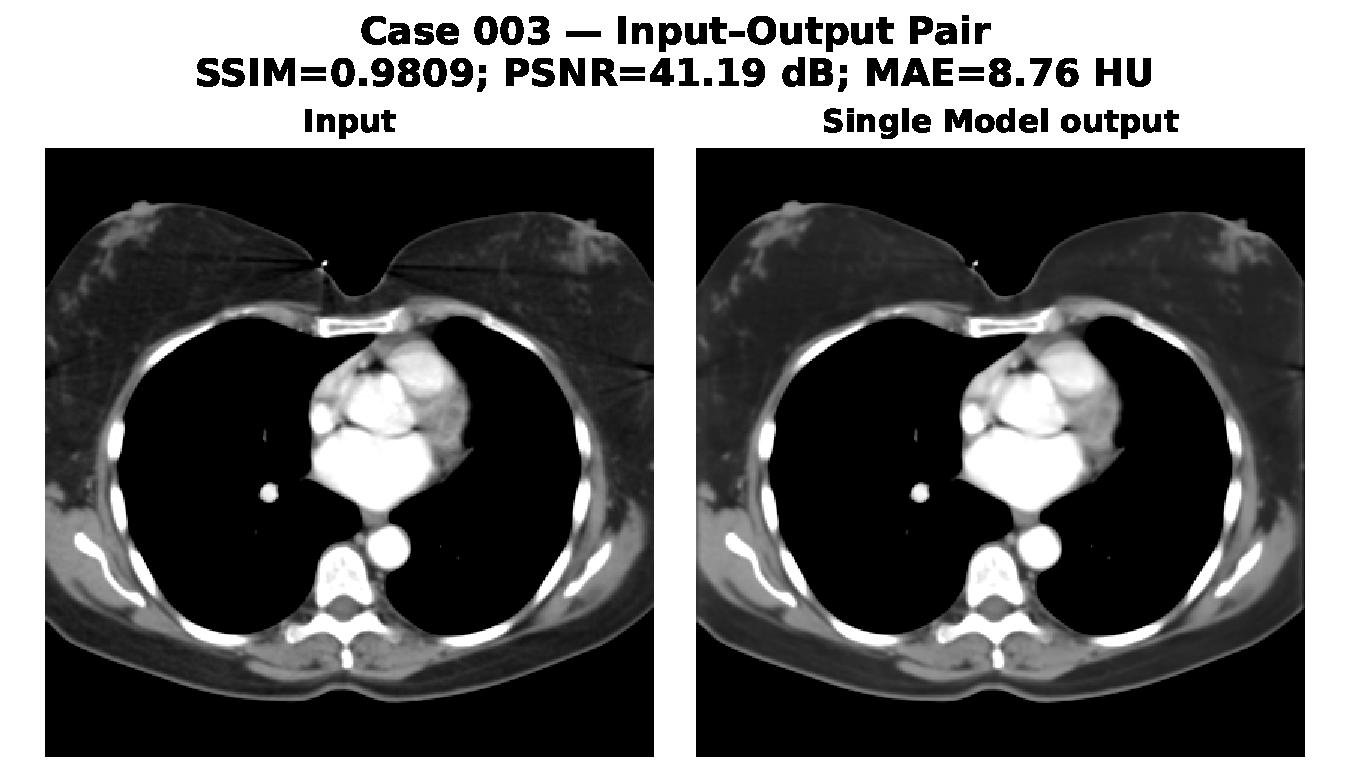
\includegraphics[width=0.84\linewidth]{Figures/Generated/external_evaluation/external_least_structurally_changed_case_003.pdf}
\end{figure}

\begin{figure}[H]
\centering
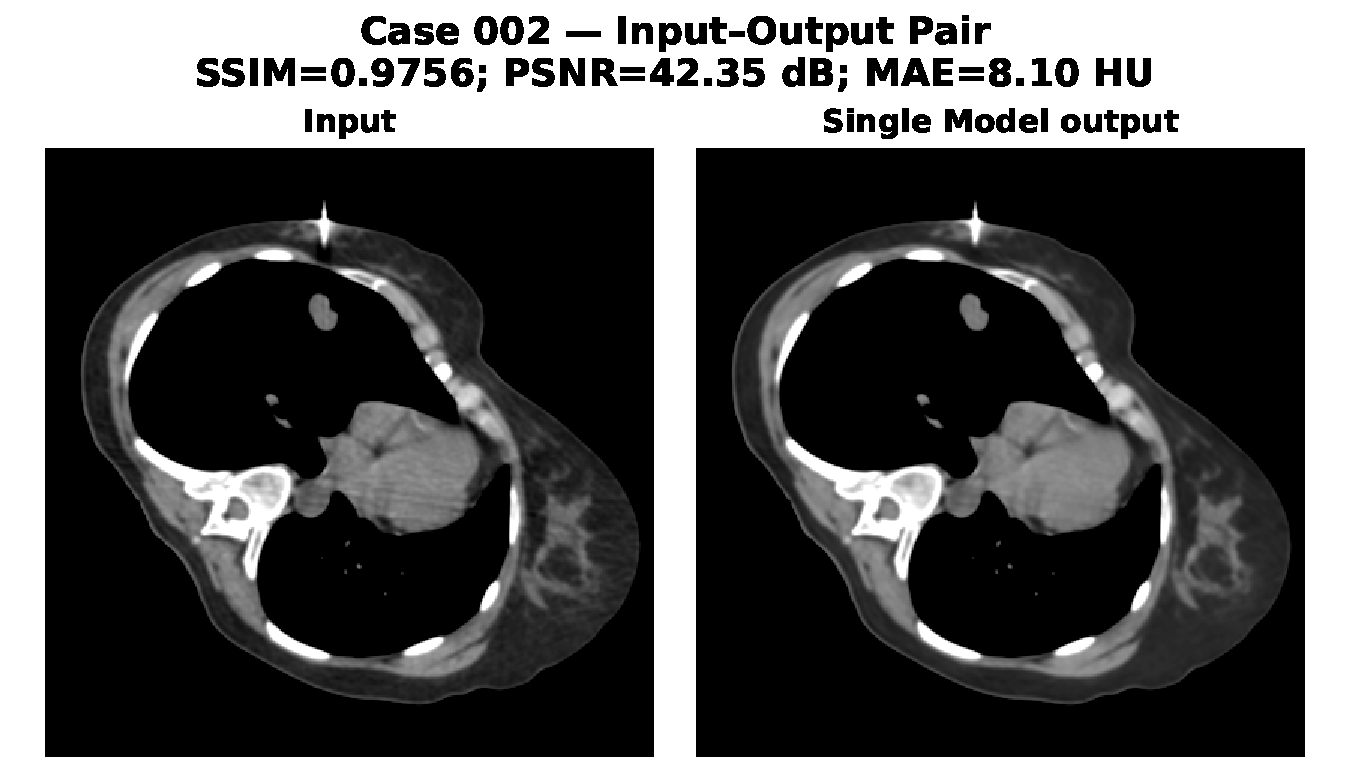
\includegraphics[width=0.84\linewidth]{Figures/Generated/external_evaluation/external_least_structurally_changed_case_002.pdf}
\end{figure}

\begin{figure}[H]
\centering
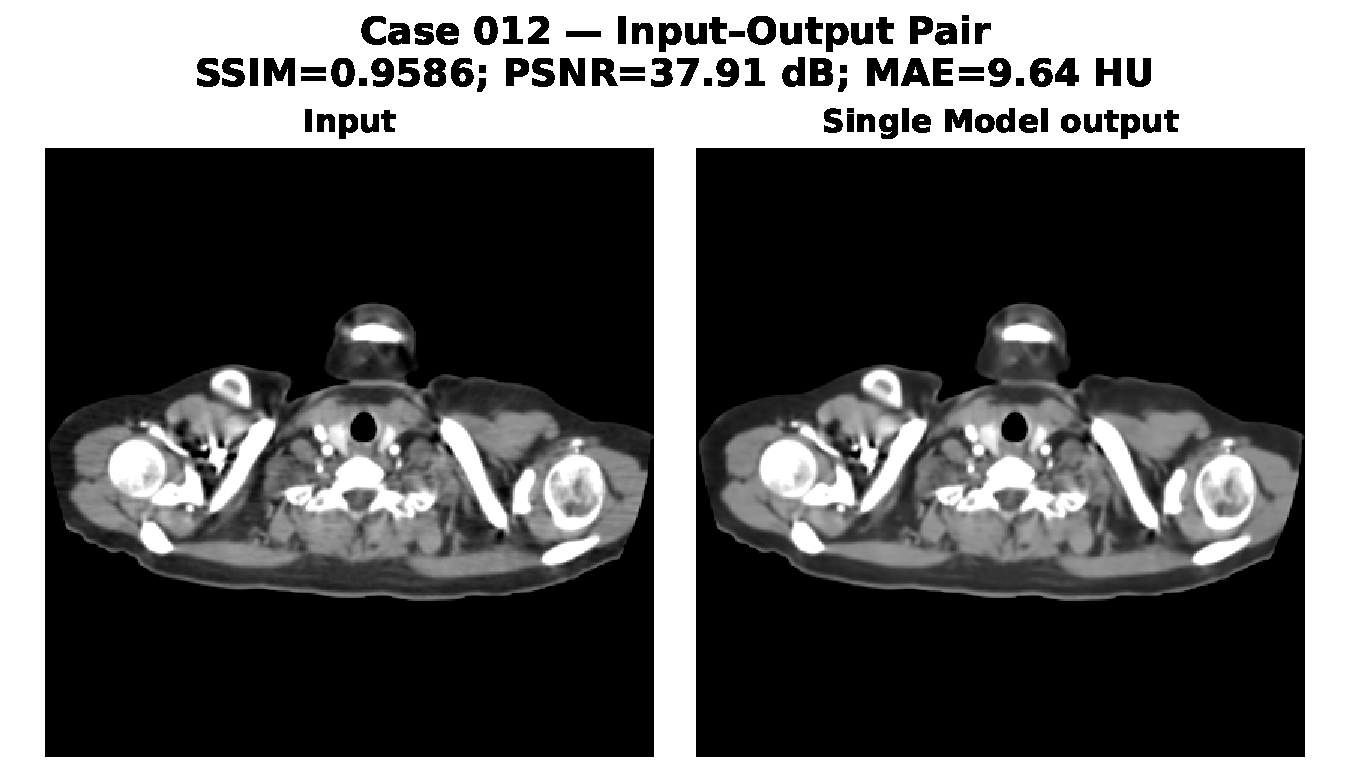
\includegraphics[width=0.84\linewidth]{Figures/Generated/external_evaluation/external_least_structurally_changed_case_012.pdf}
\end{figure}
\captionsetup{skip=1.5pt}
\captionof{figure}[Least structurally changed external cases]{External input-output pairs with the three highest SSIM values, representing the least structural change. The soft-tissue window is identical for input and output within each case.}
\label{fig:external-least-structurally-changed}
\endgroup

\begingroup
\setlength{\intextsep}{4pt}
\begin{figure}[H]
\centering
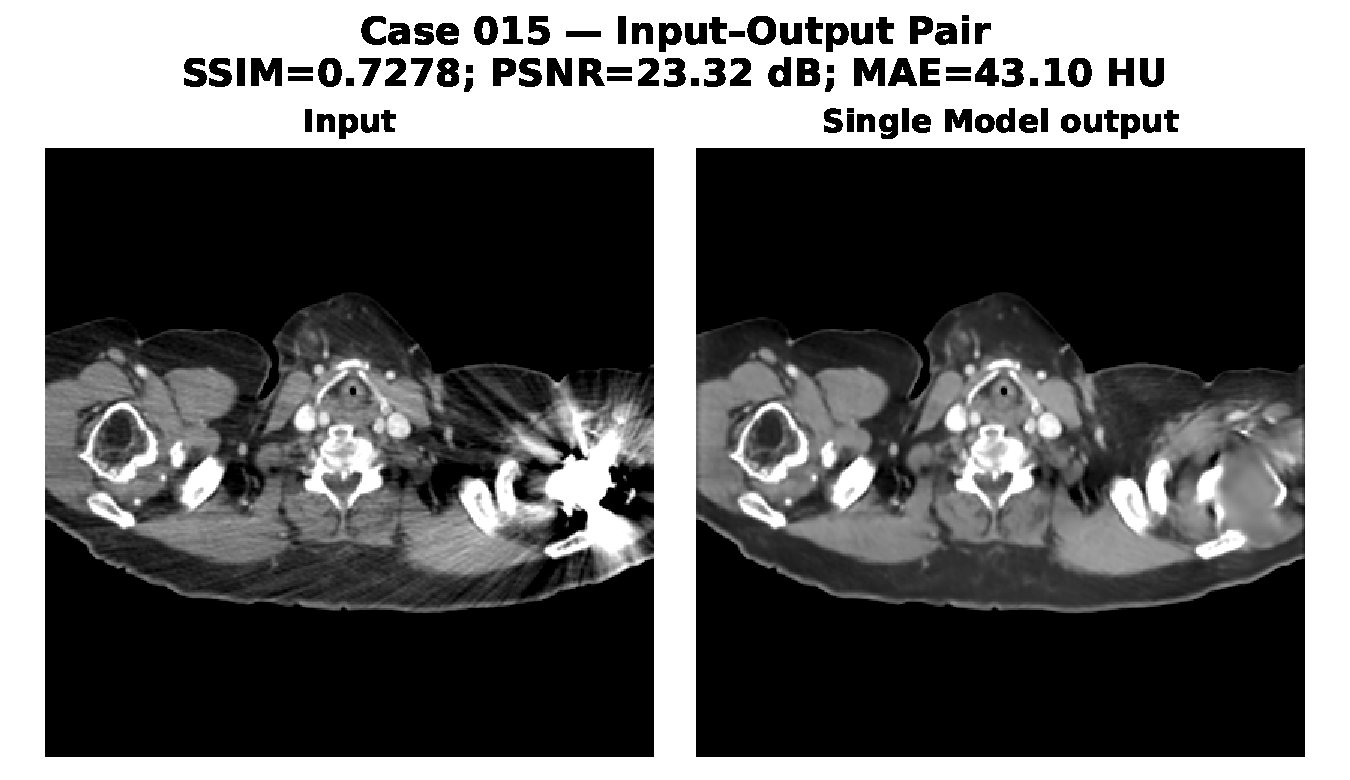
\includegraphics[width=0.84\linewidth]{Figures/Generated/external_evaluation/external_most_structurally_changed_case_015.pdf}
\end{figure}

\begin{figure}[H]
\centering
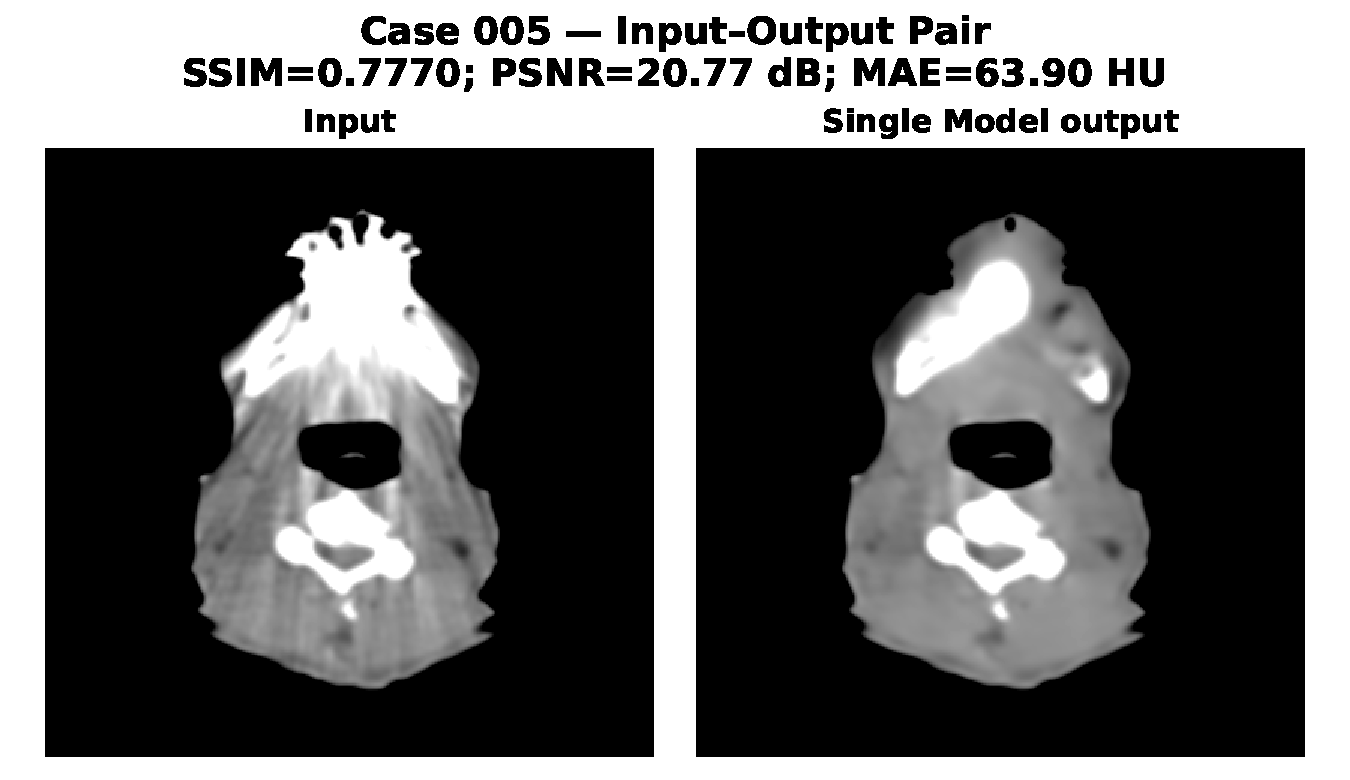
\includegraphics[width=0.84\linewidth]{Figures/Generated/external_evaluation/external_most_structurally_changed_case_005.pdf}
\end{figure}

\begin{figure}[H]
\centering
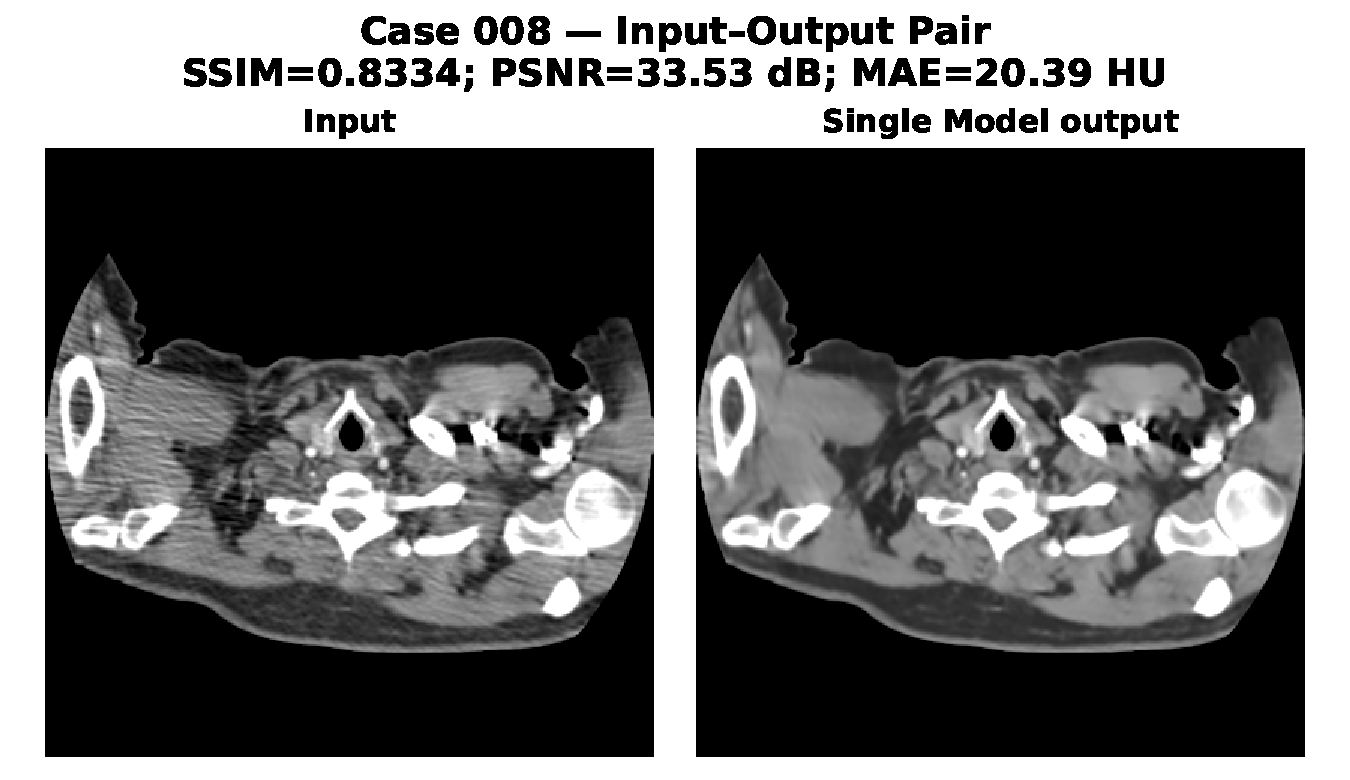
\includegraphics[width=0.84\linewidth]{Figures/Generated/external_evaluation/external_most_structurally_changed_case_008.pdf}
\end{figure}
\captionsetup{skip=1.5pt}
\captionof{figure}[Most structurally changed external cases]{External input-output pairs with the three lowest SSIM values, representing the greatest structural change. The soft-tissue window is identical for input and output within each case.}
\label{fig:external-most-structurally-changed}
\endgroup


\FloatBarrier
\subsection{Primary Outcome: Anatomical Visualization}

The primary outcome is the paired preference, per case, regarding which image better preserves the anatomical region underlying the metal artifact (``Image A'' / ``Image B'' / ``No difference''). Answers are converted back to input/output using the left/right position recorded for each case, without the reader ever knowing this mapping while answering. Training cases and hidden repeats are not part of this analysis ($n=15$ main cases per reader).

Because each doctor judges many cases, and each case is judged by many doctors, the confidence intervals were obtained with a two-way cluster bootstrap that resampled readers and cases independently. This avoids treating individual responses as fully independent. The output was more often preferred than the artifact input; the complete distribution is reported in the table.

\begin{table}[htbp]
\centering
\small
\begin{tabular}{lccc}
\toprule
\textbf{Response} & \textbf{N} & \textbf{\%} & \textbf{95\% CI} \\
\midrule
Preferred output (Single Model) & 42 & 56.0 & [28.0; 82.7] \\
Preferred input (with artifact) & 21 & 28.0 & [10.7; 48.0] \\
No difference & 12 & 16.0 & [1.3; 37.3] \\
\bottomrule
\end{tabular}
\captionsetup{skip=2pt}
\caption[Primary outcome: anatomical preservation preference]{Paired preference regarding preservation of the anatomical region underlying the metal artifact.\tablecaptionnote{Pooled frequencies over 75 valid responses (5 readers $\times$ 15 main cases). 95\% CIs are percentile intervals from a two-way cluster bootstrap over readers and cases (10,000 resamples; seed 2024).}}
\label{tab:external-primary-outcome}
\end{table}

\begin{table}[htbp]
\centering
\small
\begin{tabular}{lcc}
\toprule
\textbf{Contrast} & \textbf{Difference (pp)} & \textbf{95\% CI} \\
\midrule
Output preference $-$ input preference & $+28.0$ pp & [$-17.3$; $+70.7$] pp \\
\bottomrule
\end{tabular}
\captionsetup{skip=2pt}
\caption[Primary outcome: output--input contrast]{Cluster-bootstrap contrast for the primary outcome.\tablecaptionnote{Difference between the two pooled proportions. 95\% CI by the same two-way cluster bootstrap. A positive value favors the Single Model. No null-hypothesis test is reported because this small reader panel is interpreted descriptively.}}
\label{tab:external-primary-model}
\end{table}
\FloatBarrier

\subsection{Secondary Outcomes and Safety Perception}

The secondary outcomes use the same per-case format (``Image A'' / ``Image B'' / ``No difference''). They are reported descriptively as pooled frequencies with two-way cluster-bootstrap 95\% confidence intervals. No correction for multiple comparisons was applied.

\begin{table}[htbp]
\centering
\small
\begin{tabular}{lccc}
\toprule
\textbf{Response} & \textbf{N} & \textbf{\%} & \textbf{95\% CI} \\
\midrule
Preferred output (lower artifact intensity) & 61 & 81.3 & [65.3; 94.7] \\
Preferred input & 8 & 10.7 & [1.3; 22.7] \\
No difference & 6 & 8.0 & [0.0; 22.7] \\
\bottomrule
\end{tabular}
\captionsetup{skip=2pt}
\caption[Secondary outcome: artifact intensity]{Paired preference regarding the perceived intensity of metal artifacts.\tablecaptionnote{$n=75$ responses. 95\% CIs by two-way cluster bootstrap over readers and cases (10,000 resamples; seed 2024).}}
\label{tab:external-secondary-artifact-intensity}
\end{table}

\begin{table}[htbp]
\centering
\small
\begin{tabular}{lccc}
\toprule
\textbf{Response} & \textbf{N} & \textbf{\%} & \textbf{95\% CI} \\
\midrule
Preferred output (less distortion) & 47 & 62.7 & [38.7; 84.0] \\
Preferred input & 17 & 22.7 & [9.3; 38.7] \\
No difference & 11 & 14.7 & [1.3; 33.3] \\
\bottomrule
\end{tabular}
\captionsetup{skip=2pt}
\caption[Secondary outcome: distortion in other regions]{Paired preference regarding artifacts or anatomical distortions introduced in regions distant from the artifact.\tablecaptionnote{$n=75$ responses. 95\% CIs by two-way cluster bootstrap over readers and cases (10,000 resamples; seed 2024). This item functions as an exploratory signal of possible harm: preference for the input suggests perceived distortions or artifacts introduced by the model outside the artifact zone.}}
\label{tab:external-secondary-distortion}
\end{table}

\begin{table}[htbp]
\centering
\small
\begin{tabular}{lccc}
\toprule
\textbf{Response} & \textbf{N} & \textbf{\%} & \textbf{95\% CI} \\
\midrule
Preferred output for clinical interpretation & 42 & 56.0 & [28.0; 82.7] \\
Preferred input & 23 & 30.7 & [12.0; 53.3] \\
No difference & 10 & 13.3 & [1.3; 32.0] \\
\bottomrule
\end{tabular}
\captionsetup{skip=2pt}
\caption[Secondary outcome: clinical preference]{Paired preference regarding the image chosen for clinical interpretation.\tablecaptionnote{$n=75$ responses. 95\% CIs by two-way cluster bootstrap over readers and cases (10,000 resamples; seed 2024).}}
\label{tab:external-secondary-clinical-preference}
\end{table}

Additionally, at the end of the session, each reader answered once a 5-point ordinal question about the complementary usefulness of a version processed with this pattern relative to the original\acrshort{ct} exam (\autoref{tab:external-secondary-utility}).

\begin{table}[htbp]
\centering
\small
\begin{tabular}{lcc}
\toprule
\textbf{Category} & \textbf{N} & \textbf{\%} \\
\midrule
Definitely not & 0 & 0 \\
Probably not & 1 & 20 \\
Uncertain & 1 & 20 \\
Probably yes & 2 & 40 \\
Definitely yes & 1 & 20 \\
\bottomrule
\end{tabular}
\captionsetup{skip=2pt}
\caption[Secondary outcome: complementary utility]{Perceived complementary usefulness of a processed version relative to the original\acrshort{ct} exam.\tablecaptionnote{One response per reader (not per case). $n=5$ completed readers.}}
\label{tab:external-secondary-utility}
\end{table}
\FloatBarrier

Intra-reader consistency was assessed through two hidden repeats per reader: the same case is re-presented later in the session, without signaling, in the same left/right position as the first presentation. Because the responses are nominal and only 10 original--repeat pairs are available, the result is reported as exact agreement for each item (\autoref{tab:external-intra-reader-reliability}).

\begin{table}[htbp]
\centering
\small
\begin{tabular}{lcc}
\toprule
\textbf{Outcome} & \textbf{Exact agreement} & \textbf{Total Repetitions} \\
\midrule
Artifact intensity & 5/10 (50\%) & 10 \\
Anatomical visualization & 4/10 (40\%) & 10 \\
Other-region distortion & 4/10 (40\%) & 10 \\
Clinical preference & 5/10 (50\%) & 10 \\
\bottomrule
\end{tabular}
\captionsetup{skip=2pt}
\caption[Intra-reader repeat agreement]{Intra-reader exact agreement in the hidden repeats.\tablecaptionnote{Two cases were repeated for each of the five readers, yielding 10 paired original--repeat responses per outcome.}}
\label{tab:external-intra-reader-reliability}
\end{table}
\FloatBarrier

\subsection{Limited Interpretation to the Observational Design}

In this completed panel, the preference frequencies describe how the five readers judged these 15 cases. They do not establish a causal effect on diagnostic or therapeutic outcomes and cannot be generalized beyond this reader--case sample. The absence of a clean reference in these external cases means that the assessment of anatomical accuracy depends entirely on readers' judgment, rather than on an objective error metric. The wide cluster-bootstrap intervals, the small number of readers, and the limited repeat agreement further constrain precision and preclude meaningful subgroup analyses by specialty or experience.
